% Options for packages loaded elsewhere
\PassOptionsToPackage{unicode}{hyperref}
\PassOptionsToPackage{hyphens}{url}
\documentclass[
]{article}
\usepackage{xcolor}
\usepackage[margin=1in]{geometry}
\usepackage{amsmath,amssymb}
\setcounter{secnumdepth}{-\maxdimen} % remove section numbering
\usepackage{iftex}
\ifPDFTeX
  \usepackage[T1]{fontenc}
  \usepackage[utf8]{inputenc}
  \usepackage{textcomp} % provide euro and other symbols
\else % if luatex or xetex
  \usepackage{unicode-math} % this also loads fontspec
  \defaultfontfeatures{Scale=MatchLowercase}
  \defaultfontfeatures[\rmfamily]{Ligatures=TeX,Scale=1}
\fi
\usepackage{lmodern}
\ifPDFTeX\else
  % xetex/luatex font selection
\fi
% Use upquote if available, for straight quotes in verbatim environments
\IfFileExists{upquote.sty}{\usepackage{upquote}}{}
\IfFileExists{microtype.sty}{% use microtype if available
  \usepackage[]{microtype}
  \UseMicrotypeSet[protrusion]{basicmath} % disable protrusion for tt fonts
}{}
\makeatletter
\@ifundefined{KOMAClassName}{% if non-KOMA class
  \IfFileExists{parskip.sty}{%
    \usepackage{parskip}
  }{% else
    \setlength{\parindent}{0pt}
    \setlength{\parskip}{6pt plus 2pt minus 1pt}}
}{% if KOMA class
  \KOMAoptions{parskip=half}}
\makeatother
\usepackage{color}
\usepackage{fancyvrb}
\newcommand{\VerbBar}{|}
\newcommand{\VERB}{\Verb[commandchars=\\\{\}]}
\DefineVerbatimEnvironment{Highlighting}{Verbatim}{commandchars=\\\{\}}
% Add ',fontsize=\small' for more characters per line
\usepackage{framed}
\definecolor{shadecolor}{RGB}{248,248,248}
\newenvironment{Shaded}{\begin{snugshade}}{\end{snugshade}}
\newcommand{\AlertTok}[1]{\textcolor[rgb]{0.94,0.16,0.16}{#1}}
\newcommand{\AnnotationTok}[1]{\textcolor[rgb]{0.56,0.35,0.01}{\textbf{\textit{#1}}}}
\newcommand{\AttributeTok}[1]{\textcolor[rgb]{0.13,0.29,0.53}{#1}}
\newcommand{\BaseNTok}[1]{\textcolor[rgb]{0.00,0.00,0.81}{#1}}
\newcommand{\BuiltInTok}[1]{#1}
\newcommand{\CharTok}[1]{\textcolor[rgb]{0.31,0.60,0.02}{#1}}
\newcommand{\CommentTok}[1]{\textcolor[rgb]{0.56,0.35,0.01}{\textit{#1}}}
\newcommand{\CommentVarTok}[1]{\textcolor[rgb]{0.56,0.35,0.01}{\textbf{\textit{#1}}}}
\newcommand{\ConstantTok}[1]{\textcolor[rgb]{0.56,0.35,0.01}{#1}}
\newcommand{\ControlFlowTok}[1]{\textcolor[rgb]{0.13,0.29,0.53}{\textbf{#1}}}
\newcommand{\DataTypeTok}[1]{\textcolor[rgb]{0.13,0.29,0.53}{#1}}
\newcommand{\DecValTok}[1]{\textcolor[rgb]{0.00,0.00,0.81}{#1}}
\newcommand{\DocumentationTok}[1]{\textcolor[rgb]{0.56,0.35,0.01}{\textbf{\textit{#1}}}}
\newcommand{\ErrorTok}[1]{\textcolor[rgb]{0.64,0.00,0.00}{\textbf{#1}}}
\newcommand{\ExtensionTok}[1]{#1}
\newcommand{\FloatTok}[1]{\textcolor[rgb]{0.00,0.00,0.81}{#1}}
\newcommand{\FunctionTok}[1]{\textcolor[rgb]{0.13,0.29,0.53}{\textbf{#1}}}
\newcommand{\ImportTok}[1]{#1}
\newcommand{\InformationTok}[1]{\textcolor[rgb]{0.56,0.35,0.01}{\textbf{\textit{#1}}}}
\newcommand{\KeywordTok}[1]{\textcolor[rgb]{0.13,0.29,0.53}{\textbf{#1}}}
\newcommand{\NormalTok}[1]{#1}
\newcommand{\OperatorTok}[1]{\textcolor[rgb]{0.81,0.36,0.00}{\textbf{#1}}}
\newcommand{\OtherTok}[1]{\textcolor[rgb]{0.56,0.35,0.01}{#1}}
\newcommand{\PreprocessorTok}[1]{\textcolor[rgb]{0.56,0.35,0.01}{\textit{#1}}}
\newcommand{\RegionMarkerTok}[1]{#1}
\newcommand{\SpecialCharTok}[1]{\textcolor[rgb]{0.81,0.36,0.00}{\textbf{#1}}}
\newcommand{\SpecialStringTok}[1]{\textcolor[rgb]{0.31,0.60,0.02}{#1}}
\newcommand{\StringTok}[1]{\textcolor[rgb]{0.31,0.60,0.02}{#1}}
\newcommand{\VariableTok}[1]{\textcolor[rgb]{0.00,0.00,0.00}{#1}}
\newcommand{\VerbatimStringTok}[1]{\textcolor[rgb]{0.31,0.60,0.02}{#1}}
\newcommand{\WarningTok}[1]{\textcolor[rgb]{0.56,0.35,0.01}{\textbf{\textit{#1}}}}
\usepackage{graphicx}
\makeatletter
\newsavebox\pandoc@box
\newcommand*\pandocbounded[1]{% scales image to fit in text height/width
  \sbox\pandoc@box{#1}%
  \Gscale@div\@tempa{\textheight}{\dimexpr\ht\pandoc@box+\dp\pandoc@box\relax}%
  \Gscale@div\@tempb{\linewidth}{\wd\pandoc@box}%
  \ifdim\@tempb\p@<\@tempa\p@\let\@tempa\@tempb\fi% select the smaller of both
  \ifdim\@tempa\p@<\p@\scalebox{\@tempa}{\usebox\pandoc@box}%
  \else\usebox{\pandoc@box}%
  \fi%
}
% Set default figure placement to htbp
\def\fps@figure{htbp}
\makeatother
% definitions for citeproc citations
\NewDocumentCommand\citeproctext{}{}
\NewDocumentCommand\citeproc{mm}{%
  \begingroup\def\citeproctext{#2}\cite{#1}\endgroup}
\makeatletter
 % allow citations to break across lines
 \let\@cite@ofmt\@firstofone
 % avoid brackets around text for \cite:
 \def\@biblabel#1{}
 \def\@cite#1#2{{#1\if@tempswa , #2\fi}}
\makeatother
\newlength{\cslhangindent}
\setlength{\cslhangindent}{1.5em}
\newlength{\csllabelwidth}
\setlength{\csllabelwidth}{3em}
\newenvironment{CSLReferences}[2] % #1 hanging-indent, #2 entry-spacing
 {\begin{list}{}{%
  \setlength{\itemindent}{0pt}
  \setlength{\leftmargin}{0pt}
  \setlength{\parsep}{0pt}
  % turn on hanging indent if param 1 is 1
  \ifodd #1
   \setlength{\leftmargin}{\cslhangindent}
   \setlength{\itemindent}{-1\cslhangindent}
  \fi
  % set entry spacing
  \setlength{\itemsep}{#2\baselineskip}}}
 {\end{list}}
\usepackage{calc}
\newcommand{\CSLBlock}[1]{\hfill\break\parbox[t]{\linewidth}{\strut\ignorespaces#1\strut}}
\newcommand{\CSLLeftMargin}[1]{\parbox[t]{\csllabelwidth}{\strut#1\strut}}
\newcommand{\CSLRightInline}[1]{\parbox[t]{\linewidth - \csllabelwidth}{\strut#1\strut}}
\newcommand{\CSLIndent}[1]{\hspace{\cslhangindent}#1}
\setlength{\emergencystretch}{3em} % prevent overfull lines
\providecommand{\tightlist}{%
  \setlength{\itemsep}{0pt}\setlength{\parskip}{0pt}}
\usepackage{bookmark}
\IfFileExists{xurl.sty}{\usepackage{xurl}}{} % add URL line breaks if available
\urlstyle{same}
\hypersetup{
  pdftitle={Análisis de Datos Ómicos - PEC 2},
  pdfauthor={Beatriz Jiménez Guijarro},
  hidelinks,
  pdfcreator={LaTeX via pandoc}}

\title{Análisis de Datos Ómicos - PEC 2}
\author{Beatriz Jiménez Guijarro}
\date{22 de diciembre, 2024}

\begin{document}
\maketitle

{
\setcounter{tocdepth}{3}
\tableofcontents
}
\section{1. Introducción}\label{introducciuxf3n}

El estudio
\url{https://www.ncbi.nlm.nih.gov/geo/query/acc.cgi?acc=GSE38531}
analiza la respuesta inmunológica a infecciones por
\textbf{Staphylococcus aureus resistente a meticilina (MRSA)} mediante
datos de expresión génica obtenidos de un modelo murino (del ratón). Se
quieren comparar las condiciones de no infección e infección en
presencia o ausencia de los antibióticos linezolid y vancomicina, lo que
permite identificar cambios en la expresión génica asociados a cada
tratamiento.

El análisis se llevará a cabo en tres etapas principales: preparación de
los datos en bruto de expresión y selección de muestras, generación de
listas de genes diferencialmente expresados mediante técnicas
estadísticas, y caracterización biológica de estos genes mediante
Análisis de Enriquecimiento Genético (\emph{Gene Enrichment Analysis},
en inglés) y visualización.

Los resultados proporcionarán una caracterización clara de las
diferencias génicas entre las muestras no infectadas e infectadas, no
tratadas o tratadas con linezolid o vancomicina. Esto permitirá evaluar
el efecto inmunomodulador de ambos antibióticos, identificar rutas
biológicas afectadas y obtener una visión general de los mecanismos
moleculares subyacentes. La discusión incluye una comparación de los
perfiles génicos generados por ambos antibióticos, arrojando luz sobre
sus diferencias biológicas y aplicaciones terapéuticas.

\section{2. Objetivos del estudio}\label{objetivos-del-estudio}

El objetivo principal de este trabajo es \textbf{identificar y
caracterizar procesos biológicos relevantes a través del análisis de
expresión génica diferencial} en un conjunto de datos transcriptómicos
de ratón, integrando herramientas bioinformáticas y métodos estadísticos
robustos. Este propósito se desglosa en los siguientes objetivos
específicos:

\begin{itemize}
\item
  Pre-procesar los datos transcriptómicos para \textbf{garantizar su
  calidad}, mediante la normalización y el filtrado basado en criterios
  de variabilidad y anotación confiable.
\item
  \textbf{Identificar genes diferencialmente expresados} en muestras del
  ratón entre condiciones experimentales (muestras infectadas y no
  infectadas, sin tratar, tratadas con linezolid o tratadas con
  vancomicina), utilizando un diseño estadístico adecuado que permita
  establecer contrastes significativos y evaluar el impacto global de la
  infección (MRSA).
\item
  \textbf{Comparar los perfiles génicos} asociados a las muestras
  infectadas y no infectadas, sin tratar, tratadas con linezolid o
  tratadas con vancomicina, identificando similitudes y diferencias en
  los mecanismos moleculares y rutas biológicas moduladas por estos dos
  antibióticos.
\item
  Explorar los procesos biológicos enriquecidos asociados a los genes
  identificados mediante \textbf{Análisis de Enriquecimiento Genético}
  basado en Gene Ontology (GO) y generar representaciones gráficas
  informativas para visualizar patrones de expresión génica y su
  relación con procesos biológicos, facilitando la interpretación de
  resultados.
\end{itemize}

Estos objetivos buscan no solo alcanzar conclusiones sobre los datos
trabajados, sino también establecer un marco analítico reproducible para
estudios transcriptómicos similares.

\section{3. Materiales y Métodos}\label{materiales-y-muxe9todos}

En este apartado se describe el conjunto de datos utilizado para el
análisis, las herramientas bioinformáticas empleadas y el procedimiento
general seguido para procesar y analizar los datos de expresión génica
de los ratones.

\subsection{3.1. Origen y selección de los
datos}\label{origen-y-selecciuxf3n-de-los-datos}

El conjunto de datos utilizado en esta PEC se obtuvo de GEO, descargados
directamente desde la web del estudio
\url{https://www.ncbi.nlm.nih.gov/geo/query/acc.cgi?acc=GSE38531}, con
código GEO Serie \textbf{GSE38531}. Al final de esta web se encuentran
los enlaces para la descarga de los archivos .CEL comprimidos,
necesarios para realizar los análisis deseados. Estos archivos deben
descomprimirse para obtener cada archivo .CEL único. En nuestro caso,
utilizamos un subdirectorio llamado \texttt{GSE38531} para guardar todos
los archivos .CEL.

Este estudio consta de 35 muestras, de las que tendremos que seleccionar
algunas, 15 tomadas antes de la infección (MRSA) y 20 después: 5 de
ellas que serán las que eliminaremos, a las 2 horas de la misma y 15 a
las 24 horas. La información sobre las muestras nos fueron
proporcionados de antemano en un documento llamado
\texttt{allTargets.txt}, con el nombre de cada muestra, si estaba
infectada o no, la hora tras la infección a la que fue tomada cada
muestra (las muestras no infectadas a las 0 horas) y el tratamiento que
recibieron las muestras (ninguno, linezolid o vancomycin).

Como hemos comentado, estas muestras deben ser seleccionadas, por un
lado prescindiremos de las 5 muestras tomadas a las 2 horas y, por otro
lado, sortearemos las muestras restantes de forma que conservaremos tan
sólo 4 muestras de cada grupo.

La carga de los datos así como la selección de muestras se verán en el
apartado 4.1.1.

Para la realización del análisis también es importante saber de qué tipo
son los datos para saber qué paquete de anotaciones de Bioconductor
tendremos que utilizar. Esta información nos la proporcionará la
plataforma con la que se obtubieron los datos. Según el estudio
original, se usó la plataforma de microarrays GPL1261 {[}Mouse430\_2{]}
Affymetrix Mouse Genome 430 2.0 Array, por lo que el paquete de
anotaciones que tendremos que utilizar es
\textbf{\texttt{mouse4302.db}}.

\subsection{3.2. Herramientas y paquetes
utilizados}\label{herramientas-y-paquetes-utilizados}

El informe se llevó a cabo utilizando una variedad de herramientas
informáticas y bioinformáticas, principalmente empleando el
\textbf{lenguaje de programación R}, en su versión 4.3.3, junto con una
serie de paquetes de \textbf{Bioconductor} específicos para el análisis
de datos de microarrays. A continuación, se detallan las herramientas y
métodos utilizados en el desarrollo del informe.

Las diferentes librerías y herramientas, tanto de Bioconductor como de
R, que se han utilizado a lo largo de esta PEC han sido las instaladas
en la siguiente celda de código.

\begin{Shaded}
\begin{Highlighting}[]
\ControlFlowTok{if}\NormalTok{ (}\SpecialCharTok{!}\FunctionTok{requireNamespace}\NormalTok{(}\StringTok{"BiocManager"}\NormalTok{, }\AttributeTok{quietly =} \ConstantTok{TRUE}\NormalTok{))}
  \FunctionTok{install.packages}\NormalTok{(}\StringTok{"BiocManager"}\NormalTok{)}

\FunctionTok{install.packages}\NormalTok{(}\StringTok{"dplyr"}\NormalTok{)}
\FunctionTok{install.packages}\NormalTok{(}\StringTok{"ggplot2"}\NormalTok{)}
\FunctionTok{install.packages}\NormalTok{(}\StringTok{"ggrepel"}\NormalTok{)}
\FunctionTok{install.packages}\NormalTok{(}\StringTok{"gplots"}\NormalTok{)}
\NormalTok{BiocManager}\SpecialCharTok{::}\FunctionTok{install}\NormalTok{(}\StringTok{"Biobase"}\NormalTok{)}
\NormalTok{BiocManager}\SpecialCharTok{::}\FunctionTok{install}\NormalTok{(}\StringTok{"oligo"}\NormalTok{)}
\NormalTok{BiocManager}\SpecialCharTok{::}\FunctionTok{install}\NormalTok{(}\StringTok{"arrayQualityMetrics"}\NormalTok{)}
\NormalTok{BiocManager}\SpecialCharTok{::}\FunctionTok{install}\NormalTok{(}\StringTok{"genefilter"}\NormalTok{)}
\NormalTok{BiocManager}\SpecialCharTok{::}\FunctionTok{install}\NormalTok{(}\StringTok{"pd.mouse430.2"}\NormalTok{)}
\NormalTok{BiocManager}\SpecialCharTok{::}\FunctionTok{install}\NormalTok{(}\StringTok{"mouse4302.db"}\NormalTok{)}
\NormalTok{BiocManager}\SpecialCharTok{::}\FunctionTok{install}\NormalTok{(}\StringTok{"limma"}\NormalTok{)}
\NormalTok{BiocManager}\SpecialCharTok{::}\FunctionTok{install}\NormalTok{(}\StringTok{"AnnotationDbi"}\NormalTok{)}
\NormalTok{BiocManager}\SpecialCharTok{::}\FunctionTok{install}\NormalTok{(}\StringTok{"org.Mm.eg.db"}\NormalTok{)}
\NormalTok{BiocManager}\SpecialCharTok{::}\FunctionTok{install}\NormalTok{(}\StringTok{"clusterProfiler"}\NormalTok{)}
\NormalTok{BiocManager}\SpecialCharTok{::}\FunctionTok{install}\NormalTok{(}\StringTok{"enrichplot"}\NormalTok{)}
\end{Highlighting}
\end{Shaded}

Estas librerías y herramientas, en resumen, realizan las siguientes
funciones:

\begin{itemize}
\item
  \texttt{dplyr}: contiene algunas funciones específicas para la
  manipulación de \emph{data frames}.
\item
  \texttt{ggplot2}, \texttt{ggrepel} y \texttt{gplots}: contienen
  funciones para la visualización de datos mediante diferentes tipos de
  gráficos.
\item
  \texttt{Biobase}: proporciona clases y funciones para manejar datos
  ómicos de experimentos biológicos, especialmente para crear objetos
  \texttt{ExpressionSet} que combinan datos de expresión con información
  fenotípica.
\item
  \texttt{oligo}: se utiliza para la lectura de archivos .CEL, que son
  los datos en bruto de los microarrays, y para la normalización
  mediante el algoritmo RMA.
\item
  \texttt{limma}: implementa métodos de modelado lineal para analizar
  datos de expresión diferencial, siendo fundamental para la creación de
  matrices de diseño y contrastes, así como para la selección de genes
  diferencialmente expresados.
\item
  \texttt{arrayQualityMetrics}: ofrece herramientas para el control de
  calidad de datos de microarrays, generando informes detallados sobre
  la calidad de los arrays.
\item
  \texttt{genefilter}: se utiliza para el filtrado de genes basado en la
  variabilidad, ayudando a enfocar el análisis en las sondas más
  informativas.
\item
  \texttt{clusterProfiler} y \texttt{enrichplot}: estos paquetes
  permiten realizar y visualizar, respectivamente, análisis de
  enriquecimiento genético, ayudando a interpretar los resultados
  biológicamente.
\item
  \texttt{AnnotationDbi} y \texttt{org.Mm.eg.db}: facilitan la anotación
  de genes, mapeando identificadores de genes a sus nombres y otra
  información biológica relevante.
\end{itemize}

\subsection{3.3. Procedimiento general de
análisis}\label{procedimiento-general-de-anuxe1lisis}

El procedimiento general de análisis se desarrollará en varias etapas
clave, cada una utilizando métodos específicos para garantizar
resultados precisos y reproducibles.

Se comenzará con la \textbf{preparación de datos}, iniciando con la
carga de datos en bruto desde archivos .CEL y la preparación de un
objeto \texttt{ExpressionSet} que contendrá tanto los datos de expresión
como la información fenotípica de las muestras. También re realizará una
selección y filtrado inicial de muestras basado en los criterios
experimentales predefinidos.

Continuaremos con un \textbf{control de calidad mediante análisis
exploratorio} y con una posterior \textbf{normalización de los datos}.
Se llevará a cabo un análisis exploratorio para evaluar la calidad de
los datos mediante gráficos de boxplot, densidad, análisis de
componentes principales (PC) y clusters jerárquicos. También
utilizaremos el paquete \texttt{arrayQualityMetrics} para generar un
informe de calidad de los arrays. Finalmente, aplicaremos el algoritmo
RMA para normalizar los datos, asegurando que las intensidades de las
muestras estén en una escala comparable, y repetiremos el control de
calidad y el análisis exploratorio.

A continuación, implementaremos un \textbf{filtrado de genes} no
específicos para eliminar aquellos con baja variabilidad o sin
anotaciones relevantes, reduciendo el ruido y enfocando el análisis en
sondas informativas, y quedándonos con el 10\% de sondas que presenten
mayor variabilidad.

El siguiente paso será realizar un \textbf{análisis de expresión
diferencial}. Para ello, primero se construirán \textbf{matrices de
diseño y de contrastes} para modelar las comparaciones de interés.
Después se ajustará el \textbf{modelo lineal} de los datos normalizados
y filtrados, y se aplicarán \textbf{contrastes} para identificar genes
diferencialmente expresados. Además, visualizaremos estos resultados
mediante gráficos como \textbf{volcano plots y mapas de calor} para
visualizar patrones de expresión diferencial.

Por último, realizaremos la \textbf{anotación de los genes} y un
\textbf{análisis de significancia biológica}. Se anotarán los genes
seleccionados para obtener información biológica relevante, como
símbolos genéticos y nombres de genes y, después, realizaremos un
\textbf{Análisis de Enriquecimiento Genético} (\emph{Gene Enrichment
Analysis}, en inglés) para identificar procesos biológicos o rutas
moleculares enriquecidas en los genes expresados diferencialmente.
También se visualizarán estos resultados mediante gráficos de red
genética para interpretar los resultados en un contexto biológico.

\section{4. Desarrollo del análisis y obtención de
resultados}\label{desarrollo-del-anuxe1lisis-y-obtenciuxf3n-de-resultados}

Este es el punto clave del informe y del desarrollo de esta PEC. Dentro
de este apartado se desarrollarán todos los pasos necesarios para
realizar un anális completo de los datos a estudiar, y obtener unos
resultados en consecuencia.

\subsection{4.1. Preparación de los
datos}\label{preparaciuxf3n-de-los-datos}

Comenzaremos esta PEC preparando los datos para la realización de los
siguientes apartados. Lo primero que debemos hacer es cargar los datos y
seleccionar las muestras de la forma especificada en el enunciado y, una
vez hecho esto, proceder a la lectura de los datos en bruto. Nuestro
objetivo es crear un objeto de tipo \texttt{ExpressionSet} con los datos
en bruto y la información de las muestras, con el que desarrollaremos
los apartados de la PEC.

Para poder cargar los datos y, al mismo tiempo, asociar a cada muestra
los valores correspondientes a sus covariables, se nos ha proporcionado
el archivo \texttt{allTargets.txt} que contiene la identificación de
cada archivo .CEL (es decir, cada muestra) y su asignación a una
condición experimental específica, contando un total de 35 muestras. A
continuación, procederemos a la carga y selección de las muestras.

\subsubsection{4.1.1. Carga de los datos y selección de
muestras}\label{carga-de-los-datos-y-selecciuxf3n-de-muestras}

Para preparar los datos como se nos indica en el enunciado de este
apartado de la PEC, en primer lugar, eliminaremos del archivo
\texttt{allTargets.txt} las cinco muestras tomadas a las dos horas.

\begin{verbatim}
[1] "Muestras después de eliminar las que están a las 2 horas:"
\end{verbatim}

\begin{verbatim}
[1] "Muestras originales: 35"
\end{verbatim}

\begin{verbatim}
[1] "Muestras restantes: 30"
\end{verbatim}

\begin{verbatim}
      sample        infection    time      agent
1  GSM944831       uninfected  hour 0  untreated
2  GSM944838       uninfected  hour 0  untreated
3  GSM944845       uninfected  hour 0  untreated
4  GSM944852       uninfected  hour 0  untreated
5  GSM944859       uninfected  hour 0  untreated
6  GSM944833       uninfected  hour 0  linezolid
7  GSM944840       uninfected  hour 0  linezolid
8  GSM944847       uninfected  hour 0  linezolid
9  GSM944854       uninfected  hour 0  linezolid
10 GSM944861       uninfected  hour 0  linezolid
11 GSM944834       uninfected  hour 0 vancomycin
12 GSM944841       uninfected  hour 0 vancomycin
13 GSM944848       uninfected  hour 0 vancomycin
14 GSM944855       uninfected  hour 0 vancomycin
15 GSM944862       uninfected  hour 0 vancomycin
21 GSM944835 S. aureus USA300 hour 24  untreated
22 GSM944842 S. aureus USA300 hour 24  untreated
23 GSM944849 S. aureus USA300 hour 24  untreated
24 GSM944856 S. aureus USA300 hour 24  untreated
25 GSM944863 S. aureus USA300 hour 24  untreated
26 GSM944836 S. aureus USA300 hour 24  linezolid
27 GSM944843 S. aureus USA300 hour 24  linezolid
28 GSM944850 S. aureus USA300 hour 24  linezolid
29 GSM944857 S. aureus USA300 hour 24  linezolid
30 GSM944864 S. aureus USA300 hour 24  linezolid
31 GSM944837 S. aureus USA300 hour 24 vancomycin
32 GSM944844 S. aureus USA300 hour 24 vancomycin
33 GSM944851 S. aureus USA300 hour 24 vancomycin
34 GSM944858 S. aureus USA300 hour 24 vancomycin
35 GSM944865 S. aureus USA300 hour 24 vancomycin
\end{verbatim}

A continuación, con las muestras restantes (30 muestras) se realizará un
sorteo aleatorio mediante el cuál se conservarán tan sólo cuatro
muestras de cada combinación de grupos. Este sorteo se realizará
mediante la función \texttt{selectSamples} proporcionada en el archivo
\texttt{selectSamples.R}. Esta función extraerá un total de 24 muestras
distintas.

Sin embargo, debemos tener en cuenta que, antes de aplicar la función
\texttt{selectSamples}, tendremos que añadir los nombres de los archivos
.CEL al archvo \texttt{allTargets.txt}. Así, nos aseguraremos de que al
aplicar \texttt{selectSamples}, nos proporcionará un nuevo objeto
\texttt{targets} (valores de las covariables de las muestras
seleccionadas) únicamente con aquellos archivos .CEL seleccionados, con
el que se podrá crear un \texttt{ExpressionSet} personalizado leyendo
las 24 muestras seleccionadas. Los archivos .CEL los tenemos
descomprimidos en el directorio ``GSE38531'', dentro de nuestro
proyecto, por lo que obtendremos la lista de archivos .CEL de este
directorio.

\begin{verbatim}
                                           filenames    sample  infection
1     GSM944831_2564_6914_32297_Ctl-1_Mouse430+2.CEL GSM944831 uninfected
2     GSM944838_2564_6914_32304_Ctl-2_Mouse430+2.CEL GSM944838 uninfected
3     GSM944845_2564_6914_32311_Ctl-3_Mouse430+2.CEL GSM944845 uninfected
4     GSM944852_2564_6914_32318_Ctl-4_Mouse430+2.CEL GSM944852 uninfected
5     GSM944859_2564_6914_32325_Ctl-5_Mouse430+2.CEL GSM944859 uninfected
6 GSM944833_2564_6914_32299_Ctl-Lin-1_Mouse430+2.CEL GSM944833 uninfected
    time     agent
1 hour 0 untreated
2 hour 0 untreated
3 hour 0 untreated
4 hour 0 untreated
5 hour 0 untreated
6 hour 0 linezolid
\end{verbatim}

Una vez tenemos el nuevo \texttt{targets} con las muestras y los nombres
de los archivos .CEL correctos, podemos proceder a aplicar la función
\texttt{selectSamples} proporcionada en el archivo
\texttt{selectSamples.R}. Como comentamos antes, el objetivo de aplicar
esta función es sortear aleatoriamente las muestras para conservar tan
sólo cuatro muestras de cada combinación de grupos \emph{infection}
(infección) - \emph{agent} (tratamiento), obteniendo un total de 24
muestras diferentes. Utilizaremos como semilla (argumento \texttt{seed})
mi DNI sin la letra.

\begin{verbatim}
[1] "Muestras finales: 24"
\end{verbatim}

\begin{verbatim}
[1] "Muestras para cada combinación infection (infección) - agent (tratamiento):"
\end{verbatim}

\begin{verbatim}
                  
                   linezolid untreated vancomycin
  S. aureus USA300         4         4          4
  uninfected               4         4          4
\end{verbatim}

Para terminar de preparar los datos, dentro del archivo
\texttt{finalTargets} debemos crear dos columnas adicionales que nos
ayudarán a trabajar y analizar más fácilmente los datos en bruto, que
leeremos después. Estas columnas se llamarán \emph{shortName} y
\emph{group}.

Por un lado, \emph{shortName} obtendrá un nombre corto (como el nombre
de la columna indica, en inglés) de los nombres de los archivos .CEL,
por ejemplo, ``GSM944833\_2564\_6914\_32299\_Ctl-Lin-1\_Mouse430+2.CEL''
será en \emph{shortName} ``Ctl-Lin-1''.

Por otro lado, \emph{group} será de tipo factor y creará grupos según
las combinaciones ontenidas en la tabla de muestras anterior. Para las
muestras cuya columna \emph{infected} indica ``uninfected'', el grupo se
nombrará comenzando con ``Ctl'', y si indica ``S. aureus USA300'', el
grupo se nombrará comenzando con ``24h'', puesto que todas las muestras
que presentaban infección eran tomadas a las 24 horas de infectarse
(recordamos que aquellas que se tomaron a las 2 horas de infectarse
fueron eliminadas). Además, para las muestras cuya columna \emph{agent}
indica ``untreated'', su grupo sólo se basará en su columna
\emph{infected} puesto que no recibe tratamiento, mientras que si indica
``linezolid'' o ``vancomycin'', su grupo se nombrará finalizando con un
guión y ``Lin'' o ``Van'', respectivamente. Por ejemplo, si para una
muestra su columna \emph{infected} indica ``uninfected'' y su columna
\emph{agent} indica ``linezolid'', el nombre de su grupo será
``Ctl-Lin''.

Mostraremos el archivo final \texttt{finalTargets} para comprobar que
estas nuevas variables se han añadido correctamente y para ver las 24
muestras que se seleccionaron.

\begin{verbatim}
                                                      filenames    sample
GSM944831.1      GSM944831_2564_6914_32297_Ctl-1_Mouse430+2.CEL GSM944831
GSM944838.2      GSM944838_2564_6914_32304_Ctl-2_Mouse430+2.CEL GSM944838
GSM944845.3      GSM944845_2564_6914_32311_Ctl-3_Mouse430+2.CEL GSM944845
GSM944852.4      GSM944852_2564_6914_32318_Ctl-4_Mouse430+2.CEL GSM944852
GSM944833.6  GSM944833_2564_6914_32299_Ctl-Lin-1_Mouse430+2.CEL GSM944833
GSM944847.8  GSM944847_2564_6914_32313_Ctl-Lin-3_Mouse430+2.CEL GSM944847
GSM944854.9  GSM944854_2564_6914_32320_Ctl-Lin-4_Mouse430+2.CEL GSM944854
GSM944861.10 GSM944861_2564_6914_32327_Ctl-Lin-5_Mouse430+2.CEL GSM944861
GSM944834.11 GSM944834_2564_6914_32300_Ctl-Van-1_Mouse430+2.CEL GSM944834
GSM944841.12 GSM944841_2564_6914_32307_Ctl-Van-2_Mouse430+2.CEL GSM944841
GSM944848.13 GSM944848_2564_6914_32314_Ctl-Van-3_Mouse430+2.CEL GSM944848
GSM944855.14 GSM944855_2564_6914_32321_Ctl-Van-4_Mouse430+2.CEL GSM944855
GSM944835.16     GSM944835_2564_6914_32301_24h-1_Mouse430+2.CEL GSM944835
GSM944842.17     GSM944842_2564_6914_32308_24h-2_Mouse430+2.CEL GSM944842
GSM944849.18     GSM944849_2564_6914_32315_24h-3_Mouse430+2.CEL GSM944849
GSM944863.20     GSM944863_2564_6914_32329_24h-5_Mouse430+2.CEL GSM944863
GSM944836.21 GSM944836_2564_6914_32302_24h-lin-1_Mouse430+2.CEL GSM944836
GSM944850.23 GSM944850_2564_6914_32316_24h-lin-3_Mouse430+2.CEL GSM944850
GSM944857.24 GSM944857_2564_6914_32323_24h-lin-4_Mouse430+2.CEL GSM944857
GSM944864.25 GSM944864_2564_6914_32330_24h-lin-5_Mouse430+2.CEL GSM944864
GSM944837.26 GSM944837_2564_6914_32303_24h-Van-1_Mouse430+2.CEL GSM944837
GSM944844.27 GSM944844_2564_6914_32310_24h-Van-2_Mouse430+2.CEL GSM944844
GSM944851.28 GSM944851_2564_6914_32317_24h-Van-3_Mouse430+2.CEL GSM944851
GSM944858.29 GSM944858_2564_6914_32324_24h-Van-4_Mouse430+2.CEL GSM944858
                    infection    time      agent shortName   group
GSM944831.1        uninfected  hour 0  untreated     Ctl-1     Ctl
GSM944838.2        uninfected  hour 0  untreated     Ctl-2     Ctl
GSM944845.3        uninfected  hour 0  untreated     Ctl-3     Ctl
GSM944852.4        uninfected  hour 0  untreated     Ctl-4     Ctl
GSM944833.6        uninfected  hour 0  linezolid Ctl-Lin-1 Ctl-Lin
GSM944847.8        uninfected  hour 0  linezolid Ctl-Lin-3 Ctl-Lin
GSM944854.9        uninfected  hour 0  linezolid Ctl-Lin-4 Ctl-Lin
GSM944861.10       uninfected  hour 0  linezolid Ctl-Lin-5 Ctl-Lin
GSM944834.11       uninfected  hour 0 vancomycin Ctl-Van-1 Ctl-Van
GSM944841.12       uninfected  hour 0 vancomycin Ctl-Van-2 Ctl-Van
GSM944848.13       uninfected  hour 0 vancomycin Ctl-Van-3 Ctl-Van
GSM944855.14       uninfected  hour 0 vancomycin Ctl-Van-4 Ctl-Van
GSM944835.16 S. aureus USA300 hour 24  untreated     24h-1     24h
GSM944842.17 S. aureus USA300 hour 24  untreated     24h-2     24h
GSM944849.18 S. aureus USA300 hour 24  untreated     24h-3     24h
GSM944863.20 S. aureus USA300 hour 24  untreated     24h-5     24h
GSM944836.21 S. aureus USA300 hour 24  linezolid 24h-lin-1 24h-Lin
GSM944850.23 S. aureus USA300 hour 24  linezolid 24h-lin-3 24h-Lin
GSM944857.24 S. aureus USA300 hour 24  linezolid 24h-lin-4 24h-Lin
GSM944864.25 S. aureus USA300 hour 24  linezolid 24h-lin-5 24h-Lin
GSM944837.26 S. aureus USA300 hour 24 vancomycin 24h-Van-1 24h-Van
GSM944844.27 S. aureus USA300 hour 24 vancomycin 24h-Van-2 24h-Van
GSM944851.28 S. aureus USA300 hour 24 vancomycin 24h-Van-3 24h-Van
GSM944858.29 S. aureus USA300 hour 24 vancomycin 24h-Van-4 24h-Van
\end{verbatim}

\subsubsection{4.1.2. Lectura de datos en bruto (archivos
.CEL)}\label{lectura-de-datos-en-bruto-archivos-.cel}

Una vez que hemos obtenido correctamente las muestras que necesitamos y
hemos añadido los datos necesarios en \texttt{finalTargets}, el
siguiente paso es leer los datos en bruto a partir de los archivos .CEL.
Para ello, crearemos un objeto de tipo \texttt{ExpressionSet} para poder
combinar la información del archivo \texttt{finalTargets} con los datos
en bruto de los archivos .CEL.

Para crear este objeto, en primer lugar utilizaremos la función
\texttt{annotatedDataFrame} del paquete \texttt{Biobase} de Bioconductor
para crear un objeto de este mismo tipo con los datos de
\texttt{finalTargets}. A este nuevo objeto lo llamaremos
\texttt{dataTargets}. Se adjunta el código para que se aprecie, puesto
que no se muestra ninguna salida.

\begin{Shaded}
\begin{Highlighting}[]
\FunctionTok{library}\NormalTok{(Biobase)}

\CommentTok{\# Crear objeto de tipo "AnnotatedDataFrame" de "finalTargets"}
\NormalTok{dataTargets }\OtherTok{\textless{}{-}} \FunctionTok{AnnotatedDataFrame}\NormalTok{(finalTargets)}
\end{Highlighting}
\end{Shaded}

A partir de este nuevo objeto \texttt{dataTargets} podemos crear el
\texttt{ExpressionSet} con este objeto y los datos en bruto. Para ello,
leeremos y almacenaremos los datos en bruto de los archivos .CEL en una
variable que llamaremos \texttt{rawData}. Esta variable será el objeto
\texttt{ExpressionSet} y lo crearemos mediante la función
\texttt{read.celfiles} del paquete \texttt{oligo} de Bioconductor.

\begin{verbatim}
Reading in : GSE38531/GSM944831_2564_6914_32297_Ctl-1_Mouse430+2.CEL
Reading in : GSE38531/GSM944838_2564_6914_32304_Ctl-2_Mouse430+2.CEL
Reading in : GSE38531/GSM944845_2564_6914_32311_Ctl-3_Mouse430+2.CEL
Reading in : GSE38531/GSM944852_2564_6914_32318_Ctl-4_Mouse430+2.CEL
Reading in : GSE38531/GSM944833_2564_6914_32299_Ctl-Lin-1_Mouse430+2.CEL
Reading in : GSE38531/GSM944847_2564_6914_32313_Ctl-Lin-3_Mouse430+2.CEL
Reading in : GSE38531/GSM944854_2564_6914_32320_Ctl-Lin-4_Mouse430+2.CEL
Reading in : GSE38531/GSM944861_2564_6914_32327_Ctl-Lin-5_Mouse430+2.CEL
Reading in : GSE38531/GSM944834_2564_6914_32300_Ctl-Van-1_Mouse430+2.CEL
Reading in : GSE38531/GSM944841_2564_6914_32307_Ctl-Van-2_Mouse430+2.CEL
Reading in : GSE38531/GSM944848_2564_6914_32314_Ctl-Van-3_Mouse430+2.CEL
Reading in : GSE38531/GSM944855_2564_6914_32321_Ctl-Van-4_Mouse430+2.CEL
Reading in : GSE38531/GSM944835_2564_6914_32301_24h-1_Mouse430+2.CEL
Reading in : GSE38531/GSM944842_2564_6914_32308_24h-2_Mouse430+2.CEL
Reading in : GSE38531/GSM944849_2564_6914_32315_24h-3_Mouse430+2.CEL
Reading in : GSE38531/GSM944863_2564_6914_32329_24h-5_Mouse430+2.CEL
Reading in : GSE38531/GSM944836_2564_6914_32302_24h-lin-1_Mouse430+2.CEL
Reading in : GSE38531/GSM944850_2564_6914_32316_24h-lin-3_Mouse430+2.CEL
Reading in : GSE38531/GSM944857_2564_6914_32323_24h-lin-4_Mouse430+2.CEL
Reading in : GSE38531/GSM944864_2564_6914_32330_24h-lin-5_Mouse430+2.CEL
Reading in : GSE38531/GSM944837_2564_6914_32303_24h-Van-1_Mouse430+2.CEL
Reading in : GSE38531/GSM944844_2564_6914_32310_24h-Van-2_Mouse430+2.CEL
Reading in : GSE38531/GSM944851_2564_6914_32317_24h-Van-3_Mouse430+2.CEL
Reading in : GSE38531/GSM944858_2564_6914_32324_24h-Van-4_Mouse430+2.CEL
\end{verbatim}

Además, para facilitar la identificación de las muestras, cambiaremos
los nombres de cada fila de \texttt{dataTargets} (cada muestra) por su
nombre creado en la columna \emph{shortName} y mostraremos la
información de estos datos en bruto.

\begin{verbatim}
ExpressionFeatureSet (storageMode: lockedEnvironment)
assayData: 1004004 features, 24 samples 
  element names: exprs 
protocolData
  rowNames: Ctl-1 Ctl-2 ... 24h-Van-4 (24 total)
  varLabels: exprs dates
  varMetadata: labelDescription channel
phenoData
  rowNames: Ctl-1 Ctl-2 ... 24h-Van-4 (24 total)
  varLabels: filenames sample ... group (7 total)
  varMetadata: labelDescription channel
featureData: none
experimentData: use 'experimentData(object)'
Annotation: pd.mouse430.2 
\end{verbatim}

\begin{verbatim}
[1] TRUE
\end{verbatim}

\subsection{4.2. Análisis exploratorio y control de
calidad}\label{anuxe1lisis-exploratorio-y-control-de-calidad}

Una vez obtenidos los datos en bruto de los archivos .CEL y creado el
\texttt{ExpressionSet}, continuaremos la realización de esta PEC
realizando un análisis exploratorio de los datos y un control de calidad
de los mismo. El objetivo es explorar los datos seleccionados para
identificar patrones generales, evaluar la calidad de las muestras y
detectar posibles problemas con los datos antes de realizar un análisis
más detallado. Además, tendremos que normalizar los datos para que los
resultados de apartados posteriores sean correctos y adecuados.

\subsubsection{4.2.1. Análisis exploratorio y visualización de los datos
en
bruto}\label{anuxe1lisis-exploratorio-y-visualizaciuxf3n-de-los-datos-en-bruto}

Comenzaremos la exploración de los datos con un \textbf{análisis
univariante} que incluirá diagramas de caja (\emph{Boxplot}) y diagramas
de densidad de la señal de las muestras seleccionadas.

Para que la visualización de los datos mediante gráficos sea más
intuitiva, asignaremos a cada uno de los grupos de \texttt{rawData} un
color representativo en la variable \texttt{colors}. Para las muestras
pertenecientes al grupo \texttt{Ctl} su color será el rojo, para las
muestras pertenecientes al grupo \texttt{Ctl-Lin} su color será el
amarillo, para las muestras pertenecientes al grupo \texttt{Ctl-Van} su
color será el azul, para las muestras pertenecientes al grupo
\texttt{24h} su color será el verde, para las muestras pertenecientes al
grupo \texttt{24h-Lin} su color será el naranja y para las muestras
pertenecientes al grupo \texttt{24h-Van} su color será el morado.

Comenzamos realizando los \textbf{diagramas de caja o \emph{Boxplots}}
de los datos en \texttt{rawData}.

\pandocbounded{\includegraphics[keepaspectratio]{Jimenez_Guijarro_Beatriz_PEC2_files/figure-latex/unnamed-chunk-10-1.pdf}}

A continuación, realizamos el \textbf{diagrama de densidad} de la señal
de las muestras seleccionadas en \texttt{rawData}.

\pandocbounded{\includegraphics[keepaspectratio]{Jimenez_Guijarro_Beatriz_PEC2_files/figure-latex/unnamed-chunk-11-1.pdf}}

Tanto los diagramas de cajas (\emph{Boxplots}) como el diagrama de
densidad de la señal de los datos en bruto \texttt{rawData} muestran que
la distribución de las intensidades de las muestras son bastante
similares en cuanto a cantidad, pero sus posiciones son ligeramente
asimétricas, por lo que existe cierta variación en la intensidad de las
muestras, lo que sugiere que se debe realizar algún tipo de
normalización en los datos para centrarlos dentro de una misma escala.

Vamos a continuar la exploración de los datos con un \textbf{análisis
multivariante} que incluirá un análisis y gráfico de las componentes
principales (PC) de los datos y un diagrama jerárquico, para representar
la separación entre grupos.

Realizamos, en primer lugar, el \textbf{análisis} y el \textbf{gráfico
de las componentes principales (PC)} para los datos en bruto.

\begin{verbatim}
Importance of components:
                             PC1       PC2       PC3       PC4       PC5
Standard deviation     1.626e+05 1.123e+05 9.572e+04 8.243e+04 5.151e+04
Proportion of Variance 3.766e-01 1.796e-01 1.305e-01 9.679e-02 3.779e-02
Cumulative Proportion  3.766e-01 5.562e-01 6.867e-01 7.835e-01 8.213e-01
                             PC6       PC7       PC8       PC9      PC10
Standard deviation     4.695e+04 4.038e+04 3.686e+04 3.478e+04 3.282e+04
Proportion of Variance 3.140e-02 2.323e-02 1.935e-02 1.723e-02 1.535e-02
Cumulative Proportion  8.527e-01 8.759e-01 8.952e-01 9.125e-01 9.278e-01
                            PC11      PC12      PC13      PC14      PC15
Standard deviation     2.916e+04 2.514e+04 2.363e+04 2.307e+04 2.183e+04
Proportion of Variance 1.211e-02 9.000e-03 7.950e-03 7.580e-03 6.790e-03
Cumulative Proportion  9.399e-01 9.489e-01 9.569e-01 9.645e-01 9.713e-01
                            PC16      PC17      PC18      PC19      PC20
Standard deviation     1.969e+04 1.669e+04 1.646e+04 1.618e+04 1.553e+04
Proportion of Variance 5.520e-03 3.970e-03 3.860e-03 3.730e-03 3.440e-03
Cumulative Proportion  9.768e-01 9.808e-01 9.846e-01 9.883e-01 9.918e-01
                            PC21      PC22     PC23      PC24
Standard deviation     1.451e+04 1.408e+04 1.30e+04 9.872e-09
Proportion of Variance 3.000e-03 2.820e-03 2.41e-03 0.000e+00
Cumulative Proportion  9.948e-01 9.976e-01 1.00e+00 1.000e+00
\end{verbatim}

El análisis de componentes principales (PC) nos indica que la primera
componente (PC1) nos explica más del 37\% de la variabilidad de los
datos y que no se explica más de un 80\% de la variabilidad de los datos
hasta la componente 5 (PC5), por lo que es posible encontrar un pequeño
efecto \emph{batch} en los datos, pero lo comprobaremos mejor cuando
realicemos el gráfico. También podemos observar que se explica el 100\%
de la variabilidad de los datos en la componente 23 (PC23), por lo que
la última componente (PC24) no aporta variabilidad adicional porque
tiene una desviación estándar cercana a cero.

Realicemos ahora el gráfico. Para la realización de este gráfico de
componentes principales (PC), utilizaremos una función diseñada
específicamente para ello, obtenida directamente de la bibliografía. A
raíz de esta función, obtendremos el gráfico correspondiente.

\pandocbounded{\includegraphics[keepaspectratio]{Jimenez_Guijarro_Beatriz_PEC2_files/figure-latex/unnamed-chunk-14-1.pdf}}

Como hemos puntualizado anteriormente, la primera componente principal
(PC1) repesenta el 37,7\% de la variabilidad total de los datos, y como
podemos observar en el gráfico de los datos en bruto en las dos primeras
componentes principales, esta variabilidad está principalmente atribuida
a la condición de \textbf{infección} (\emph{infection}), ya que las
muestras que no han sido infectadas con S. aureus USA300 (es decir,
tomadas a las 0 horas de la infección) están a la izquierda del gráfico,
mientras que las muestras que sí han sido infectadas con S. aureus
USA300 (es decir, tomadas a las 24 horas de la infección) están a la
derecha del gráfico. Sin embargo, es posible que exista un pequeño
efecto \emph{batch} dado que hay algunas muestras de diferentes grupos
de infección que están en el centro del gráfico.

Vamos a realizar el \textbf{diagrama o clúster jerárquico} para
confirmar o desmentir esta teoría y ver más adecuadamente la separación
entre grupos de los datos en bruto.

\pandocbounded{\includegraphics[keepaspectratio]{Jimenez_Guijarro_Beatriz_PEC2_files/figure-latex/unnamed-chunk-15-1.pdf}}

El diagrama o clúster jerárquico nos muestra una \textbf{clara
separación} entre los grupos que presentan infección de S. aureus USA300
(a las 24 horas) y aquellos que no presentan infección, por lo que no
tenemos un claro efecto \emph{batch} que debiésemos eliminar. Además,
las muestras \texttt{24h-2} y \texttt{24h-2} se separan de todas las
demás, por lo que podrían ser eliminadas del análisis, sin embargo, no
las eliminaremos para tener un análisis más completo.

\subsubsection{4.2.2. Control de calidad de los datos en
bruto}\label{control-de-calidad-de-los-datos-en-bruto}

Para realizar el control de calidad de los datos en bruto
\texttt{rawData} que nos indica el enunciado de este apartado, vamos a
utilizar el paquete \texttt{arrayQualityMetrics}. Este paquete contiene
los diferentes tipos de análisis exploratorios que hemos realizado hasta
ahora, como, por ejemplo, los diagramas de cajas o \emph{Boxplots} o el
análisis de componentes principales (PC), entre otros. Así, se pueden
ejecutar varios tipos de análisis diferentes de manera más sencilla y
rápida. Para realizar este control de calidad, utilizaremos la función
\texttt{arrayQualityMetrics} del paquete del mismo nombre antes
mencionado. Esta función realizará todos los análisis, generando un
informe con los resultados obtenidos y posibles problemas detectados.

Al ejecutar la función \texttt{arrayQualityMetrics}, le indicaremos que
el informe del control de calidad generado se guarde en un subdirectorio
de nombre \texttt{arrayQualityMetrics\_PEC2} para facilitar su búsqueda
en el directorio principal. También indicaremos mediante el parámetro
\texttt{intgroup} que se utilice el factor infección o \emph{infection}
como separador de colores en los gráficos, puesto que hemos visto en el
partado anterior que este es el factor que produce la mayor diferencia
entre las muestras.

El informe generado dentro de este subdirectorio se nombra
automáticamente como \texttt{index.html}, y dentro del mismo se
encuentran todos los análisis y resultados generados por la función
\texttt{arrayQualityMetrics}.

Una de las primeras cosas que encontramos en el informe
\texttt{index.html} es una tabla con unas columnas denominadas como
\texttt{*1}, \texttt{*2} y \texttt{*3}. Estas columnas indican algunos
criterios de calidad que deben ser verificados para comprobar que los
arrays son de ``buena calidad''. En nuestro caso, se han marcado sólo
dos muestras una vez. Normalmente cuando sólo hay una marca significa
que los problemas o \emph{outliers} potenciales son pequeños por lo que
no hace falta eliminar estos arrays. Para nuestro análisis, podemos
decidir mantener todos los arrays. A continuación mostramos la tabla en
cuestión obtenida en el informe \texttt{index.html}.

\begin{figure}
\centering
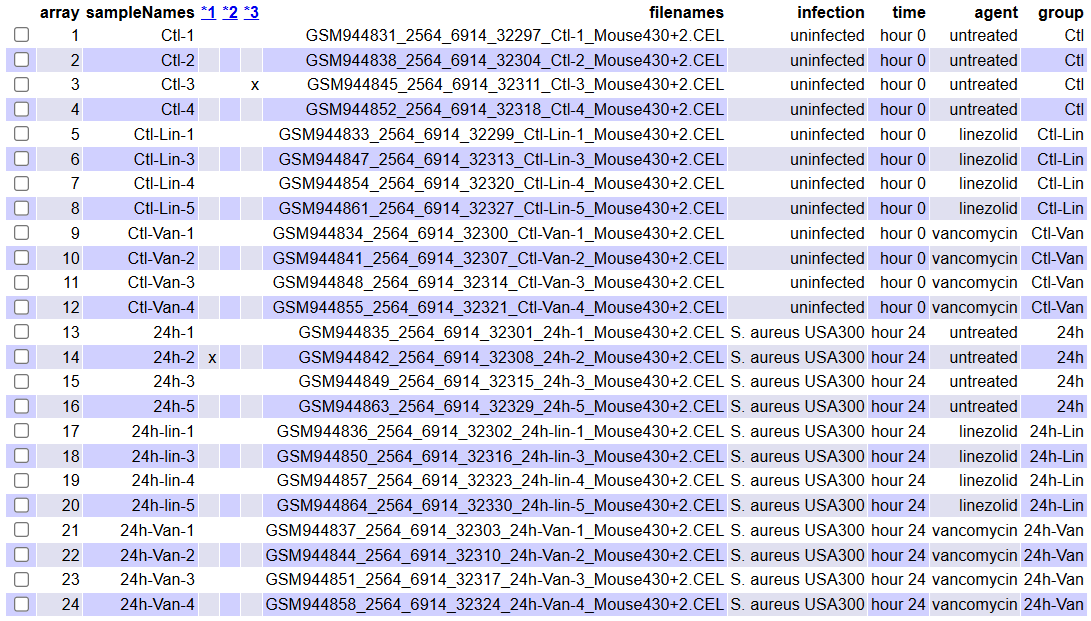
\includegraphics[width=5.20833in,height=\textheight,keepaspectratio]{arrayQualityMetrics.png}
\caption{Imagen 1. Control de calidad de los datos en bruto}
\end{figure}

\subsubsection{4.2.3. Análisis de efecto batch de los datos en
bruto}\label{anuxe1lisis-de-efecto-batch-de-los-datos-en-bruto}

Como hemos analizado en el apartado 4.2.1, no hemos detectado un efecto
\emph{batch} preocupante en los datos puesto que podemos apreciar una
clara separación atribuida a la condición de \textbf{infección}
(\emph{infection}), la cuál se muestra como la principal fuente de
variabilidad en las muestras. Las muestras no infectadas están divididas
en un grupo totalmente separado de las muestras infectadas con S. aureus
USA300, lo que implica que existen diferencias demostrables entre ambos
grupos y que este factor (la infección) no se cruza con el factor
tratamiento o \emph{agent}.

Si realizamos un \textbf{análisis basado en diatancias}, podremos ver
como estas conclusiones son correctas. Calcularemos la matriz de
distancias y la visualizaremos mediante un mapa de colores o
\emph{heatmap}.

\pandocbounded{\includegraphics[keepaspectratio]{Jimenez_Guijarro_Beatriz_PEC2_files/figure-latex/unnamed-chunk-17-1.pdf}}

Efectivamente, confirmamos que no se aprecia un efecto \emph{batch} y
que, por lo tanto, no hay que eliminarlo.

\subsubsection{4.2.4. Normalización de los datos en
bruto}\label{normalizaciuxf3n-de-los-datos-en-bruto}

Una vez hemos realizado el análisis exploratorio y el control de calidad
de los datos en bruto \texttt{rawData}, y hemos concluido además que los
datos presentan una ligera asimetría, lo que indica que existe cierta
variación en la intensidad de las muestras, debemos proceder a realizar
una \textbf{normalización de los datos}. Esto es importante porque, para
realizar el análisis de expresión diferencial, es necesario hacer que
las muestras sean comparables entre sí e intentar reducir y, si es
posible eliminar, toda la variabilidad en las muestras que no se deba a
razones biológicas, ya que lo que nos interesará descubrir en los
siguientes apartados son las diferencias de intensidad que reflejen
únicamente la expresión diferencial de los genes, y no otras cuestiones.

Como en el enunciado del apartado nos indica que utilicemos el algoritmo
RMA, normalizaremos los datos en bruto mediante la función \texttt{rma}
obtenida del paquete \texttt{oligo}, que utilizamos para leer los datos
en bruto. Los datos normalizados seguirán siendo un objeto del tipo
\texttt{ExpressionSet}, como comprobamos al mostrar su información
general.

\begin{verbatim}
Background correcting
Normalizing
Calculating Expression
\end{verbatim}

\begin{verbatim}
ExpressionSet (storageMode: lockedEnvironment)
assayData: 45101 features, 24 samples 
  element names: exprs 
protocolData
  rowNames: Ctl-1 Ctl-2 ... 24h-Van-4 (24 total)
  varLabels: exprs dates
  varMetadata: labelDescription channel
phenoData
  rowNames: Ctl-1 Ctl-2 ... 24h-Van-4 (24 total)
  varLabels: filenames sample ... group (7 total)
  varMetadata: labelDescription channel
featureData: none
experimentData: use 'experimentData(object)'
Annotation: pd.mouse430.2 
\end{verbatim}

\subsubsection{4.2.5. Análisis exploratorio y visualización de los datos
normalizados}\label{anuxe1lisis-exploratorio-y-visualizaciuxf3n-de-los-datos-normalizados}

Una vez que ya tenemos los datos normalizados en un nuevo objeto de tipo
\texttt{ExpressionSet} llamado \texttt{esetData\_rma}, vamos a realizar
el mismo análisis exploratorio que realizamos para los datos en bruto en
el apartado 4.2.1, para comprobar que la intensidad de los datos
normalizados ya no presenta la asimetría que presentaban los datos en
bruto.

Como hicimos anteriormente, comenzaremos con el \textbf{análisis
univariante} que incluye los \textbf{diagramas de caja (\emph{Boxplot})}
y el \textbf{diagrama de densidad} de la señal de las muestras
normalizadas.

\pandocbounded{\includegraphics[keepaspectratio]{Jimenez_Guijarro_Beatriz_PEC2_files/figure-latex/unnamed-chunk-19-1.pdf}}

\pandocbounded{\includegraphics[keepaspectratio]{Jimenez_Guijarro_Beatriz_PEC2_files/figure-latex/unnamed-chunk-20-1.pdf}}

Como podemos ver tanto en los diagramas de cajas (\emph{Boxplots}) como
en el diagrama de densidad de la señal de los datos normalizados, ya no
presentan la asimetría que mostraban los datos en bruto y que se ha
mitigado la variación en la intensidad de las muestras, por lo que
podemos decir que los datos se han normalizado y escalado correctamente.

Si realizamos el \textbf{análisis multivariante} con los datos
normalizados, realizando de nuevo un \textbf{análisis y gráfico de las
componentes principales (PC)} y un \textbf{diagrama jerárquico} para
representar la separación entre grupos, obtenemos los siguientes
resultados.

\begin{verbatim}
Importance of components:
                           PC1     PC2     PC3     PC4     PC5      PC6     PC7
Standard deviation     43.8904 23.4531 20.9496 14.8206 12.7402 10.96564 9.70567
Proportion of Variance  0.4569  0.1305  0.1041  0.0521  0.0385  0.02852 0.02234
Cumulative Proportion   0.4569  0.5873  0.6914  0.7435  0.7820  0.81055 0.83289
                          PC8     PC9    PC10    PC11   PC12    PC13    PC14
Standard deviation     8.7600 8.48216 8.06846 7.29095 7.0530 6.68843 6.46645
Proportion of Variance 0.0182 0.01706 0.01544 0.01261 0.0118 0.01061 0.00992
Cumulative Proportion  0.8511 0.86816 0.88360 0.89620 0.9080 0.91861 0.92853
                         PC15    PC16    PC17    PC18    PC19    PC20    PC21
Standard deviation     6.2942 6.11554 5.99419 5.87054 5.76391 5.70006 5.62740
Proportion of Variance 0.0094 0.00887 0.00852 0.00817 0.00788 0.00771 0.00751
Cumulative Proportion  0.9379 0.94680 0.95532 0.96349 0.97137 0.97908 0.98659
                          PC22    PC23      PC24
Standard deviation     5.48590 5.14360 9.374e-14
Proportion of Variance 0.00714 0.00627 0.000e+00
Cumulative Proportion  0.99373 1.00000 1.000e+00
\end{verbatim}

En este caso, el análisis de componentes principales (PC) nos indica que
la primera componente (PC1) nos explica más del 45\% de la variabilidad
de los datos, es decir, ha aumentado en comparación con los datos en
bruto, y que no se explica más de un 80\% de la variabilidad de los
datos hasta la componente 6 (PC6) en este caso. Igual que en el caso
anterior, se explica el 100\% de la variabilidad de los datos en la
componente 23 (PC23), por lo que la última componente (PC24) no aporta
variabilidad adicional porque tiene una desviación estándar cercana a
cero.

Observemos el gráfico de componentes principales (PC) de los datos
normalizados a continuación.

\pandocbounded{\includegraphics[keepaspectratio]{Jimenez_Guijarro_Beatriz_PEC2_files/figure-latex/unnamed-chunk-22-1.pdf}}

La primera componente principal (PC1) repesenta ahora el 45,7\% de la
variabilidad total de los datos, por lo que ha aumentado
considerablemente y como podemos observar en el gráfico de los datos
normalizados en las dos primeras componentes principales, esta
variabilidad sigue estando principalmente atribuida a la condición de
\textbf{infección} (\emph{infection}). De hecho, ahora se puede apreciar
mucho mejor la separación entre las muestras que no han sido infectadas
con S. aureus USA300 (es decir, tomadas a las 0 horas de la infección)
que están a la izquierda del gráfico, y las muestras que sí han sido
infectadas con S. aureus USA300 (es decir, tomadas a las 24 horas de la
infección) están a la derecha del gráfico. Podemos decir que las
muestras normalizadas no muestran ningún tipo de efecto \emph{batch}
dado que ahora todas las muestras están completamente separadás según su
tipo de infección.

Vamos a corroborar esto mediante el diagrama o clúster jerárquico.

\pandocbounded{\includegraphics[keepaspectratio]{Jimenez_Guijarro_Beatriz_PEC2_files/figure-latex/unnamed-chunk-23-1.pdf}}

Efectivamente, el diagrama o clúster jerárquico nos muestra una
\textbf{clara separación} entre los grupos que presentan infección de S.
aureus USA300 (a las 24 horas) y aquellos que no presentan infección,
por lo que no tenemos efecto \emph{batch}. Además, las muestras
\texttt{24h-2} y \texttt{24h-2} ya no están separadas de las demás,
están unidas a su grupo de infección y ya no haría falta plantear su
eliminación.

\subsubsection{4.2.6. Control de calidad de los datos
normalizados}\label{control-de-calidad-de-los-datos-normalizados}

Vamos a realizar un nuevo \textbf{control de calidad}, pero esta vez de
los \textbf{datos normalizados} \texttt{esetData\_rma}, de la misma
manera que hicimos en el apartado 4.2.2, ejecutando la función
\texttt{arrayQualityMetrics}, e indicado esta vez que el informe del
control de calidad generado se guarde en un subdirectorio de nombre
\texttt{arrayQualityMetrics\_Norm\_PEC2}. También indicaremos mediante
el parámetro \texttt{intgroup} que se utilice el factor infección o
\emph{infection} como separador de colores en los gráficos.

En este caso, la tabla del informe \texttt{index.html} generado solo
muestra una muestra marcada, aunque dos veces esta vez. Sin embargo,
esto no indica que haya que eliminar el array puesto que los diagramas
del apartado anterior indican que esta muestra está relacionadas con las
demás de su grupo, por lo que estos posibles problemas o \emph{outliers}
potenciales deben ser pequeños, por lo que no hace falta eliminar este
array. Para nuestro análisis, decidirmos mantener todos los arrays.

\begin{figure}
\centering
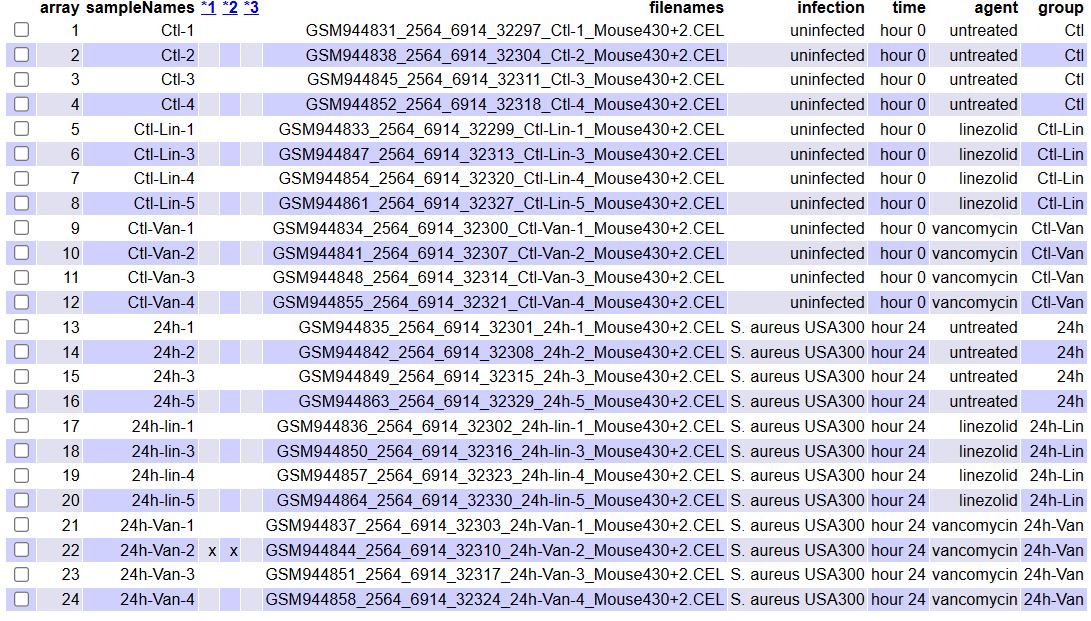
\includegraphics[width=5.20833in,height=\textheight,keepaspectratio]{arrayQualityMetrics_Norm.png}
\caption{Imagen 2. Control de calidad de los datos en bruto}
\end{figure}

\subsection{4.3. Filtrado de los datos}\label{filtrado-de-los-datos}

En este apartado vamos a realizar un filtraje no específico de los datos
que hemos normalizado en el apartado 4.2.4, \texttt{esetData\_rma}. El
objetivo de este filtraje es eliminar aquellos genes o aquellos
\emph{spots} cuyas imágenes o señales sean erróneas por diferentes
motivos, con el fin de reducir el ruído de fondo. Este proceso ayudará a
enfocar el análisis en aquellas sondas cuyos niveles de expresión varían
más entre las muestras, asumiendo que las sondas con baja variabilidad
no aportan mucha información biológicamente relevante, o que no existe
una anotación específica para esos genes.

Para realizar el filtrado de los datos, utilizaremos la función
\texttt{nsFilter} del paquete \texttt{genefilter} de Bioconductor. Esta
función elimina genes en función de un umbral de variabilidad, y en este
caso, el enunciado nos indica que nos quedemos con el 10\% de sondas que
presenten mayor variabilidad, por lo que el umbral \texttt{var.cutoff}
que tendremos que indicar será del 0,9, es decir, eliminaremos el 90\%
de las sondas menos variables.

Si hay un paquete de anotaciones disponible (que asocie identificadores
de conjuntos de sondas e identificadores de genes de diferentes bases de
datos), también se puede utilizar para eliminar conjuntos de sondas que
no tengan un identificador de gen asociado. En nuestro caso, nuestro
objeto \texttt{esetData\_rma} sí que disponía de un paquete de
anotaciones, concretamente \texttt{pd.mouse430.2}, sin embargo, la base
datos de anotaciones correcta para este paquete es
\texttt{mouse4302.db}, por lo que tendremos que modificar el campo
\texttt{annotation} de \texttt{esetData\_rma} por esta base de datos
para que la función \texttt{nsFilter} pueda filtrar con el parámetro
\texttt{require.entrez\ =\ TRUE} y se rellenen las anotaciones
(\texttt{annotation}) con \texttt{mouse4302.db}. Este parámetro lo que
nos permitirá es eliminar aquellos genes que no tengan identificador en
la base de datos \texttt{Entrez}, para poder obtener sólo el 10\% de
sondas que presenten mayor variabilidad de las que sí tengan
identificador en la base de datos.

La función \texttt{nsFilter} devuelve un objeto de tipo
\texttt{ExpressionSet} con los valores filtrados y un informe de los
resultados del filtrado llamado \texttt{filter.log}.

\begin{verbatim}
[1] "eset"       "filter.log"
\end{verbatim}

Comprobemos que los valores filtrados son, efectivamente, un objeto
\texttt{ExpressionSet} y la información contenida en este objeto.

\begin{verbatim}
[1] "ExpressionSet"
attr(,"package")
[1] "Biobase"
\end{verbatim}

\begin{verbatim}
ExpressionSet (storageMode: lockedEnvironment)
assayData: 2049 features, 24 samples 
  element names: exprs 
protocolData
  rowNames: Ctl-1 Ctl-2 ... 24h-Van-4 (24 total)
  varLabels: exprs dates
  varMetadata: labelDescription channel
phenoData
  rowNames: Ctl-1 Ctl-2 ... 24h-Van-4 (24 total)
  varLabels: filenames sample ... group (7 total)
  varMetadata: labelDescription channel
featureData: none
experimentData: use 'experimentData(object)'
Annotation: mouse4302.db 
\end{verbatim}

En cuanto al informe de los resultados, \texttt{filter.log}, este tiene
la siguiente estructura e información.

\begin{verbatim}
$numDupsRemoved
[1] 16958

$numLowVar
[1] 18442

$numRemoved.ENTREZID
[1] 7639

$feature.exclude
[1] 13
\end{verbatim}

El informe del filtrado nos indica que, de las 45101 \emph{features}
iniciales que había en el objeto \texttt{esetData\_rma}, se han
eliminado 16958 sondas por estar duplicadas según el identificador
EntrezID (\texttt{numDupsRemoved}), se han eliminado 18442 sondas por
tener baja variabilidad en los datos (\texttt{numLowVar}), se han
eliminado 7639 sondas porque no tenían un ID Entrez asociado
(\texttt{numRemoved.ENTREZID}) y también se han eliminado otras 13
sondas porque coincidían con el patrón definido en
\texttt{feature.exclude}, es decir, las sondas cuyo identificador
comenzaba con \texttt{"\^{}AFFX"} (sondas de control usadas por
Affymetrix).

Todo esto nos deja con un \textbf{total de 2049 \emph{features} o genes}
anotados que tienen la mayor variabilidad, y será con los que se
realizarán los análisis de genes diferencialmente expresados.

Para finalizar este apartado, en primer lugar almacenaremos los genes
restantes en la variable \texttt{esetData\_filtered} de la siguiente
manera (adjunto el código para que se aprecie, puesto que no se muestra
ninguna salida).

\begin{Shaded}
\begin{Highlighting}[]
\CommentTok{\# Almacenar genes filtrados en "esetData\_filtered"}
\NormalTok{esetData\_filtered }\OtherTok{\textless{}{-}}\NormalTok{filtered}\SpecialCharTok{$}\NormalTok{eset}
\end{Highlighting}
\end{Shaded}

Y, en segundo y último lugar, vamos a guardar, en un subdirectorio
llamado \texttt{results}, los objetos normalizados y filtrados,
\texttt{esetData\_rma} y \texttt{esetData\_filtered}, respectivamente,
en un archivo binario al que llamaremos
\texttt{normalized.filtered.Data.Rda}, para hacer uso de estos datos en
futuros análisis, si fuera necesario. También guardaremos (en el mismo
subdirectorio) los valores de expresión, tanto de los datos normalizados
como de los datos filtrados, en archivos .csv, de nombres
\texttt{normalized.Data.csv} y \texttt{filtered.Data.csv},
respectivamente.

\subsection{4.4. Construcción de las matrices de diseño y de
contrastes}\label{construcciuxf3n-de-las-matrices-de-diseuxf1o-y-de-contrastes}

En este apartado vamos a realizar las matrices de diseño y de contrastes
que utilizaremos para llevar a cabo las comparaciones propuestas que
son:

\begin{itemize}
\tightlist
\item
  Infectados vs no infectados sin tratamiento.
\item
  Infectados vs no infectados tratados con LINEZOLID.
\item
  Infectados vs no infectados tratados con VANCOMICINA.
\end{itemize}

Estas comparaciones generarán tres listas de genes que tendremos que,
por un lado, caracterizar mediante análisis de significación biológica
y, por otro lado, comparar entre ellas. El objetivo final es intentar
caracterizar, a través del cambio en la expresión génica, el efecto de
la infección y del tratamiento con antibióticos así como comparar los
efectos de éstos. Para ello, se utilizará el método de Modelos Lineales
para Microarrays presentado por Smyth (2004), implementado en el paquete
\texttt{limma}, para seleccionar genes expresados diferencialmente. Pero
esto se hará en apartados posteriores.

Pero por el momento, nos centraremos en los primeros pasos para el
análisis basado en modelos lineales es crear la matriz de diseño y la
matriz de contrastes.

\subsubsection{4.4.1. Matriz de diseño}\label{matriz-de-diseuxf1o}

La \textbf{matriz de diseño} es una tabla que describe la asignación de
cada muestra a un grupo o condición experimental. Esta tabla asigna un 1
a cada muestra dentro del grupo específico al que pertenece, y un 0 a
las demás. Las filas de esta tabla son las muestras analizadas, mientras
que las columnas representan los diferentes grupos.

La matriz de diseño puede configurarse de manera manual o generarse a
partir de una variable factorial incluida en los \texttt{targets} creado
para tal fin. Recordamos que, en el apartado 4.1.1 ya creamos esta
variable factorial que se incluyó en el archivo \texttt{dataTargets} y
que denominamos \emph{group}. También recordaremos que esta variable
representa la combinación de las dos condiciones experimentales que nos
interesan en el estudio, \emph{infection} (``uninfected'' y ``S. aureus
USA300'') y \emph{agent} (``untreated'', ``linezolid'' y
``vancomycin''), las cuales se integran como un factor con seis niveles.

Es importante recordar también cómo se configuró esta variable
\emph{group}, puesto que utilizaremos las mismas denominaciones a la
hora de realizar tanto la matriz de diseño como la de contrastes:

\begin{itemize}
\tightlist
\item
  Para las muestras cuya columna \emph{infected} indica ``uninfected'',
  el grupo se nombrará comenzando con ``Ctl'', y si indica ``S. aureus
  USA300'', el grupo se nombrará comenzando con ``24h'', puesto que
  todas las muestras que presentaban infección eran tomadas a las 24
  horas de infectarse (recordamos que aquellas que se tomaron a las 2
  horas de infectarse fueron eliminadas). Además, para las muestras cuya
  columna \emph{agent} indica ``untreated'', su grupo sólo se basará en
  su columna \emph{infected} puesto que no recibe tratamiento, mientras
  que si indica ``linezolid'' o ``vancomycin'', su grupo se nombrará
  finalizando con un guión y ``Lin'' o ``Van'', respectivamente. Por
  ejemplo, si para una muestra su columna \emph{infected} indica
  ``uninfected'' y su columna \emph{agent} indica ``linezolid'', el
  nombre de su grupo será ``Ctl-Lin''.
\end{itemize}

Sin embargo, para evitar errores con los grupos denominados con ``24h''
a la hora de realizar la matriz de contrastes (puesto que lo reconoce
como un número y no como un nombre), cambiaremos la denominación ``24h''
por \textbf{``inf24h''} en las matrices. También utilizaremos
\textbf{puntos} en vez de guiones.

Creamos, a continuación, la matriz de diseño con la función
\texttt{model.matrix} y la variable factorial \emph{group} de los datos
filtrados en el apartado 4.3, \texttt{esetData\_filtered}.

\begin{verbatim}
          Ctl Ctl.Lin Ctl.Van inf24h inf24h.Lin inf24h.Van
Ctl-1       1       0       0      0          0          0
Ctl-2       1       0       0      0          0          0
Ctl-3       1       0       0      0          0          0
Ctl-4       1       0       0      0          0          0
Ctl-Lin-1   0       1       0      0          0          0
Ctl-Lin-3   0       1       0      0          0          0
Ctl-Lin-4   0       1       0      0          0          0
Ctl-Lin-5   0       1       0      0          0          0
Ctl-Van-1   0       0       1      0          0          0
Ctl-Van-2   0       0       1      0          0          0
Ctl-Van-3   0       0       1      0          0          0
Ctl-Van-4   0       0       1      0          0          0
24h-1       0       0       0      1          0          0
24h-2       0       0       0      1          0          0
24h-3       0       0       0      1          0          0
24h-5       0       0       0      1          0          0
24h-lin-1   0       0       0      0          1          0
24h-lin-3   0       0       0      0          1          0
24h-lin-4   0       0       0      0          1          0
24h-lin-5   0       0       0      0          1          0
24h-Van-1   0       0       0      0          0          1
24h-Van-2   0       0       0      0          0          1
24h-Van-3   0       0       0      0          0          1
24h-Van-4   0       0       0      0          0          1
attr(,"assign")
[1] 1 1 1 1 1 1
attr(,"contrasts")
attr(,"contrasts")$group
[1] "contr.treatment"
\end{verbatim}

\subsubsection{4.4.2. Matriz de contrastes}\label{matriz-de-contrastes}

Una vez obtenida la matriz de diseño, podemos pasar a obtener la
\textbf{matriz de contrastes}. Recordamos que son tres las comparaciones
que queremos hacer (definidas al inicio del apartado 4.4), lo que
equivale a tres contrastes.

La matriz de contrastes se emplea para representar las comparaciones
entre distintos grupos de interés. Su estructura consta de un número de
columnas igual al de comparaciones a realizar realizadas y de filas
equivalentes a los grupos o columnas de la matriz de diseño. Cada
comparación entre grupos, denominada ``contraste'', se expresa mediante
un 1 y un -1 en las filas correspondientes a los grupos en comparación,
mientras que las demás filas se completan con 0. En caso de incluir
varios grupos en una comparación, se asignan tantos coeficientes como
grupos involucrados, con la única condición de que la suma de estos
coeficientes sea igual a cero.

Para realizar la matriz de contrastes utilizaremos la función
\texttt{makeContrasts} del paquete \texttt{limma} de Bioconductor. Los
grupos a contrastar se definirían de la siguiente manera, según las
comparaciones que nos indica el enunciado:

\begin{itemize}
\tightlist
\item
  Infectados vs no infectados sin tratamiento = inf24h vs Ctl.
\item
  Infectados vs no infectados tratados con LINEZOLID = inf24h-Lin vs
  Ctl-Lin.
\item
  Infectados vs no infectados tratados con VANCOMICINA = inf24h-Van vs
  Ctl-Van.
\end{itemize}

\begin{verbatim}
            Contrasts
Levels       inf24h_vs_Ctl inf24h.Lin_vs_Ctl.Lin inf24h.Van_vs_Ctl.Van
  Ctl                   -1                     0                     0
  Ctl.Lin                0                    -1                     0
  Ctl.Van                0                     0                    -1
  inf24h                 1                     0                     0
  inf24h.Lin             0                     1                     0
  inf24h.Van             0                     0                     1
\end{verbatim}

\subsection{4.5. Obtención de las listas de genes diferencialmente
expresados para cada
comparación}\label{obtenciuxf3n-de-las-listas-de-genes-diferencialmente-expresados-para-cada-comparaciuxf3n}

En este apartado, y una vez definidas la matriz de diseño y la matriz de
contrastes, en primer lugar procederemos a estimar el modelo lineal para
microarrays necesario, implementado en el paquete \texttt{limma} de
Bioconductor, y estimar los contrastes para seleccionar los genes
expresados diferencialmente. A continuación, obtendremos listas de genes
expresados diferencialmente para cada comparación y visualizaremos esta
expresión diferencial mediante \emph{volcano plots}. Finalizaremos el
apartado realizando las comparaciones entre las listas de genes, tanto
gráficamente como con la función \texttt{decideTests} del paquete
\texttt{limma}, y visualizando los perfiles de expresión mediante mapas
de calor o \emph{Heatmaps}.

\subsubsection{4.5.1. Estimación del modelo y selección de
genes}\label{estimaciuxf3n-del-modelo-y-selecciuxf3n-de-genes}

El modelo implementado en el paquete \texttt{limma} proporciona las
estadísticas de prueba habituales, como los p-valores ajustados o los
\emph{Fold-change t-moderated}, que se utilizan para ordenar los genes
de mayor a menor diferencialmente expresados.

Obtendremos el modelo mediante la función \texttt{lmFit}, al cuál
aplicaremos los contrastes obtenidos en la matriz de contrastes
(apartado 4.4.2). Además, para controlar el porcentaje de falsos
positivos que pueden resultar de un gran número de contrastes realizados
simultáneamente, los p-valores se ajustan de manera que tengamos control
sobre la tasa de falsos positivos utilizando el método de Benjamini y
Hochberg, es decir, mediante la estimación bayesiana, que se puede
realizar mediante la función \texttt{eBayes}.

El objeto final obtenido, al que denominaremos \texttt{fit\_contrasts},
será de clase \texttt{MArrayLM}.

\begin{verbatim}
[1] "MArrayLM"
attr(,"package")
[1] "limma"
\end{verbatim}

\subsubsection{4.5.2. Obtención de listas de genes expresados
diferencialmente}\label{obtenciuxf3n-de-listas-de-genes-expresados-diferencialmente}

Para obtener las listas de genes expresados diferencialmente para cada
una de las comparaciones mencionadas en el apartado 4.4, utilizaremos la
función \texttt{topTable} del paquete \texttt{limma}, que genera, para
cada uno de los contrastes dados, una lista de genes ordenados desde el
p-valor más pequeño hasta el más grande, es decir, desde el gen mayor
hasta el gen menor diferencialmente expresado.

La función \texttt{topTable} proporciona las siguientes estadísticas
para cada gen en cada contraste:

\begin{itemize}
\item
  \texttt{logFC} (\emph{Log Fold Change}): representa la diferencia de
  medias entre las condiciones comparadas, en escala logarítmica. Un
  valor positivo indica que el gen está más expresado en el grupo de
  referencia y un valor negativo indica que el gen está menos expresado.
\item
  \texttt{AveExpr}: el promedio de los niveles de expresión del gen en
  todas las muestras incluidas en la comparación.
\item
  \texttt{t}: estadístico-t, calculado en el análisis lineal, que mide
  la diferencia relativa entre los niveles de expresión en los grupos
  comparados.
\item
  \texttt{P.Value}: p-valor asociado con la prueba estadística.
\item
  \texttt{adj.P.Val}: p-valor ajustado para múltiples pruebas usando el
  método de Benjamini-Hochberg. Este valor es clave para identificar
  genes significativamente diferenciados con base en un umbral (por
  ejemplo, 0,05).
\item
  \texttt{B}: estadística ``B'' que representa la probabilidad de que el
  gen sea diferencialmente expresado, en escala logarítmica. Valores
  positivos indican que es más probable que el gen sea diferencialmente
  expresado.
\end{itemize}

Pasemos, por lo tanto, a obtener las listas de genes expresados
diferencialmente. Como estas listas tienden a ser muy extensas,
mostraremos una cabecera de cada una.

\textbf{Comparación 1: Infectados vs no infectados sin tratamiento}

Se trata de genes que cambian su expresión entre ``24h'' y ``Ctl'' para
el tipo de tratamiento (\emph{agent}) ``untreated''.

\begin{verbatim}
                logFC   AveExpr        t      P.Value    adj.P.Val        B
1421262_at   7.924139  7.218665 22.34134 3.365476e-16 6.054344e-13 27.08754
1427747_a_at 6.486822 10.735477 21.73073 5.909560e-16 6.054344e-13 26.55481
1422953_at   4.155073 11.293155 18.86744 1.020818e-14 6.972185e-12 23.82176
1440865_at   4.622099 11.206482 18.02917 2.530550e-14 1.296274e-11 22.93945
1418722_at   6.282290 10.993838 17.51931 4.477451e-14 1.834860e-11 22.38237
1449366_at   4.987598 10.194740 17.11963 7.075434e-14 2.416261e-11 21.93435
\end{verbatim}

\textbf{Comparación 2: Infectados vs no infectados tratados con
LINEZOLID}

Se trata de genes que cambian su expresión entre ``24h-Lin'' y
``Ctl-Lin'' para el tipo de tratamiento (\emph{agent}) ``linezolid''.

\begin{verbatim}
                 logFC   AveExpr         t      P.Value    adj.P.Val        B
1421262_at    6.236835  7.218665  17.58415 4.160683e-14 8.525240e-11 22.27818
1427747_a_at  4.986680 10.735477  16.70528 1.148378e-13 1.176513e-10 21.32192
1440865_at    3.440354 11.206482  13.41961 8.049199e-12 5.497603e-09 17.23690
1422953_at    2.834734 11.293155  12.87201 1.772723e-11 7.800821e-09 16.46585
1416301_a_at -2.602025  6.920170 -12.82350 1.903568e-11 7.800821e-09 16.39614
1418722_at    4.507239 10.993838  12.56925 2.774432e-11 9.474684e-09 16.02700
\end{verbatim}

\textbf{Comparación 3: Infectados vs no infectados tratados con
VANCOMICINA}

Se trata de genes que cambian su expresión entre ``24h-Van'' y
``Ctl-Van'' para el tipo de tratamiento (\emph{agent}) ``vancomycin''.

\begin{verbatim}
                 logFC   AveExpr         t      P.Value    adj.P.Val        B
1421262_at    6.768573  7.218665  19.08333 8.127044e-15 1.665231e-11 23.89304
1427747_a_at  4.918189 10.735477  16.47584 1.508370e-13 1.545325e-10 21.11976
1418722_at    5.039160 10.993838  14.05261 3.334707e-12 1.684166e-09 18.11622
1440865_at    3.581953 11.206482  13.97193 3.724321e-12 1.684166e-09 18.00801
1416301_a_at -2.820530  6.920170 -13.90036 4.109726e-12 1.684166e-09 17.91153
1437060_at    4.793432  7.708000  13.02794 1.412032e-11 4.822091e-09 16.69822
\end{verbatim}

La primera columna de cada tabla superior contiene el ID del fabricante,
Affymetrix, para cada conjunto de muestras. En próximos apartados,
cuando anotemos los genes, comprobaremos qué gen corresponde a cada ID
de Affymetrix.

\subsubsection{4.5.3. Visualización de la expresión diferencial para
cada
comparación}\label{visualizaciuxf3n-de-la-expresiuxf3n-diferencial-para-cada-comparaciuxf3n}

Podemos obtener una visualización de la expresión diferencial general de
los genes de cada comparación utilizando \emph{volcano plots}. En estos
gráficos se muestra la cantidad de genes que presentan un cambio
significativo en su expresión, y si este número es alto o bajo. El eje X
indica los cambios de expresión en una escala logarítmica, reflejando el
``efecto biológico'', mientras que el eje Y muestra el ``logaritmo
negativo'' del p-valor o, de forma alternativa, la estadística B, lo que
corresponde al ``efecto estadístico''.

Realizaremos un \emph{volcano plot} para cada una de las comparaciones,
como hicimos en el apartado 4.5.2 con las \texttt{topTable}. Para ello,
utilizaremos la función \texttt{volcanoplot}. Para obtener los símbolos
genéticos asociados a las sondas dentro de cada \emph{volcano plot},
seleccionaremos, mediante la función \texttt{select}, aquellos símbolos
(argumento \texttt{SYMBOL}) correspondientes a los genes de nuestro
modelo \texttt{fit\_contrasts}. Para ello, necesitaremos acceder a la
base de datos correspondiente a las muestras, que como sabemos, es
\texttt{mouse4302.db}. Además, dentro de cada gráfico resaltaremos los 6
genes más significativos (con mayor expresión diferencial) de cada
comparación, que coincidirán con aquellos obtenidos en las primeras 6
posiciones de su \texttt{topTable} correspondiente.

\textbf{\emph{Volcano plot} 1: Infectados vs no infectados sin
tratamiento}

Se trata de genes que cambian su expresión entre ``24h'' y ``Ctl'' para
el tipo de tratamiento (\emph{agent}) ``untreated''.

\pandocbounded{\includegraphics[keepaspectratio]{Jimenez_Guijarro_Beatriz_PEC2_files/figure-latex/unnamed-chunk-37-1.pdf}}

\textbf{\emph{Volcano plot} 2: Infectados vs no infectados tratados con
LINEZOLID}

Se trata de genes que cambian su expresión entre ``24h-Lin'' y
``Ctl-Lin'' para el tipo de tratamiento (\emph{agent}) ``linezolid''.

\pandocbounded{\includegraphics[keepaspectratio]{Jimenez_Guijarro_Beatriz_PEC2_files/figure-latex/unnamed-chunk-38-1.pdf}}

\textbf{\emph{Volcano plot} 3: Infectados vs no infectados tratados con
VANCOMICINA}

Se trata de genes que cambian su expresión entre ``24h-Van'' y
``Ctl-Van'' para el tipo de tratamiento (\emph{agent}) ``vancomycin''.

\pandocbounded{\includegraphics[keepaspectratio]{Jimenez_Guijarro_Beatriz_PEC2_files/figure-latex/unnamed-chunk-39-1.pdf}}

\subsubsection{4.5.4. Comparaciones
múltiples}\label{comparaciones-muxfaltiples}

En este apartado vamos a realizar las comparaciones múltiples entre
genes. Al realizarlas, resulta útil identificar cuáles han sido
seleccionados en cada caso. En ciertos escenarios, los genes de mayor
relevancia biológica serán aquellos que se seleccionan únicamente en una
comparación, pero no en las demás. Por el contrario, en otras
situaciones, el interés puede centrarse en los genes seleccionados de
manera consistente en todas las comparaciones.

Realizaremos estas comparaciones múltiples, en primer lugar, con la
función \texttt{decideTests} del paquete \texttt{limma}. Esta función
crea una tabla con tantas columnas como comparaciones y tantas filas
como genes. Esta tabla contiene, para cada gen y cada comparación, un 1
si se trata de una regulación positiva significativa o \texttt{up} (el
gen esta sobre-expresado en esa condicion), un 0 si no hay una
diferencia significativa o \texttt{notSig}, o un -1 si se trata de una
regulación a la baja significativa o \texttt{down} (el gen esta
infra-expresado en esa condicion). Pondremos un umbral del p-valor menor
a 0,1 y un LogFC (mínimo \emph{fold-change}) mayor a 1.

Como visulizar la tabla entera es inviable debido a la gran cantidad de
genes que hay, mostraremos un resumen del análisis contando las filas
(los genes) que tienen como mínimo una celda distinta de cero.

\begin{verbatim}
       inf24h_vs_Ctl inf24h.Lin_vs_Ctl.Lin inf24h.Van_vs_Ctl.Van
Down             412                   590                   922
NotSig           671                   568                   458
Up               529                   454                   232
\end{verbatim}

Ahora realizaremos, en segundo lugar, las comparaciones múltiples de
manera gráfica utilizando un diagrama de Venn mediante la función
\texttt{vennDiagram}. El diagrama de Venn visualiza la tabla resumen
anterior, obtenida del análisis realizado mediante \texttt{decideTests}.

El diagrama de Venn representa la cantidad de genes que se consideran
expresados diferencialmente en cada comparación, aplicando un umbral
específico (en este caso, p-valor \textless{} 0.1 y logFC \textgreater{}
1, especidicado en la función \texttt{decideTests}). A continuación
mostraremos este diagrama que ilustra cuántos de estos genes son comunes
entre una o varias condiciones.

\pandocbounded{\includegraphics[keepaspectratio]{Jimenez_Guijarro_Beatriz_PEC2_files/figure-latex/unnamed-chunk-42-1.pdf}}

Los \textbf{resultados} que obtenemos a raiz de las comparaciones
múltiples realizadas son los siguientes:

\begin{itemize}
\item
  \textbf{Infectados vs no infectados sin tratamiento}: hay un
  \textbf{equilibrio relativo} entre genes con regulación positiva
  (\texttt{Up}) y a la baja (\texttt{Down}), aunque ligeramente
  \textbf{más genes están activados en las muestras infectadas} que en
  las no infectadas. Además, muchos genes no son significativos
  (\texttt{NotSig}), lo que sugiere una cantidad moderada de cambios
  específicos por la infección sin tratar.
\item
  \textbf{Infectados vs no infectados tratados con LINEZOLID}: hay
  ligeramente \textbf{más genes con regulación a la baja}
  (\texttt{Down}) en comparación con los activados o con regulación
  positiva (\texttt{Up}), lo que podría indicar un \textbf{efecto del
  Linezolid} hacia la regulación negativa de la expresión génica.
\item
  \textbf{Infectados vs no infectados tratados con VANCOMICINA}: tiene
  la \textbf{mayor proporción de genes con regulación a la baja}
  (\texttt{Down}), lo que sugiere un \textbf{efecto más fuerte del
  tratamiento con Vancomicina} sobre la regulación negativa.
\end{itemize}

En conclusión, estos resultados sugieren que cada comparación (sin
tratamiento, con Linezolid o con Vancomicina) tiene un impacto único
sobre la expresión génica, siendo evidente que la diferencia más clara
se encuentra entre \textbf{Infectados vs no infectados tratados con
VANCOMICINA}, aunque es relevante mencionar que las otras dos
condiciones también muestran bastante diferencia, siendo la que menos
diferencia muestra la condición Infectados vs no infectados tratados con
LINEZOLID.

\subsubsection{\texorpdfstring{4.5.5. Visualización de los perfiles de
expresión mediante mapas de calor o
\emph{Heatmaps}}{4.5.5. Visualización de los perfiles de expresión mediante mapas de calor o Heatmaps}}\label{visualizaciuxf3n-de-los-perfiles-de-expresiuxf3n-mediante-mapas-de-calor-o-heatmaps}

Una vez que se han seleccionado los genes que son diferencialmente
expresados, podemos visualizar los diferentes perfiles de expresión
(alto, bajo o no significativo) de estos genes mediante un mapa de calor
o \emph{heatmap}. Esta visualización se hace sin un orden específico,
pero suele ser preferible representarlos mediante una agrupación
jerárquica de los genes en filas y/o las muestras en columnas, con el
objetivo de identificar conjuntos de genes que muestren patrones
similares de variación y que potencialmente puedan asociarse con los
distintos grupos en comparación.

En cuanto a los genes que debemos seleccionar para el mapa de calor, en
nuestro caso seleccionaremos los genes que se han seleccionado en el
partado anterior (4.5.4), es decir, los genes que se han denominado
expresados diferencialmente en, al menos, una de las tres comparaciones,
\texttt{res\_selected}.

Una vez tenemos los genes seleccionados, generaremos un mapa de calor
con agrupamiento de genes y muestras, utilizando los parámetros
\texttt{Rowv\ =\ TRUE} para el agrupamiento de genes (filas), y
\texttt{Colv\ =\ TRUE} para el agrupamiento de muestras (columnas); y el
parámetro \texttt{dendrogram\ =\ "both"} para visualizar estos
agrupamientos mediante dendogramas (clusters jerárquicos).

\pandocbounded{\includegraphics[keepaspectratio]{Jimenez_Guijarro_Beatriz_PEC2_files/figure-latex/unnamed-chunk-44-1.pdf}}

\subsection{4.6. Anotacion de los genes}\label{anotacion-de-los-genes}

Al obtener las \texttt{topTable} de los genes expresados
diferencialmente para cada una de las comparaciones propuestas, en el
apartado 4.5.2, estas nos arrojaron listas de genes basados en los
identificadores originales del fabricante, Affymetrix. Es este apartado,
debemos anotar estos genes, comprobando qué gen corresponde a cada ID de
Affymetrix. Este proceso denominado \textbf{anotación} busca información
para asociar los identificadores que aparecen en la \texttt{topTable},
generalmente correspondientes a conjuntos de sondas o transcripciones
según el tipo de matriz, con nombres más comprensibles o fácilmente
identificables. En nuestro caso, asociaremos a los identificadores
originales los nombres procedentes de, por ejemplo, \textbf{``Symbol''},
\textbf{``EntrezID''}, \textbf{``EnsemblID''} y \textbf{``Gename''}.

En primer lugar, vamos a comprobar que en la base de datos de las
anotaciones correspondiente a nuestro estudio, \texttt{mouse4302.db}
contenga los tipos de anotación que deseamos obtener para los genes.

\begin{verbatim}
 [1] "ACCNUM"       "ALIAS"        "ENSEMBL"      "ENSEMBLPROT"  "ENSEMBLTRANS"
 [6] "ENTREZID"     "ENZYME"       "EVIDENCE"     "EVIDENCEALL"  "GENENAME"    
[11] "GENETYPE"     "GO"           "GOALL"        "IPI"          "MGI"         
[16] "ONTOLOGY"     "ONTOLOGYALL"  "PATH"         "PFAM"         "PMID"        
[21] "PROBEID"      "PROSITE"      "REFSEQ"       "SYMBOL"       "UNIPROT"     
\end{verbatim}

Efectivamente podremos encontrar los cuatro tipos de anotaciones
mencionados para los genes de las \texttt{topTable} de este estudio.

Ahora podremos pasar a realizar estas anotaciones. Para ello,
utilizaremos la función \texttt{select} del paquete
\texttt{AnnotationDbi} de Bioconductor. Dentro de la función
seleccionaremos la base de datos \texttt{mouse4302.db}, los nombres de
las filas de cada \texttt{topTable}, es decir, los genes seleccionados
que se deben anotar, y los tipos de anotaciones que queremos obtener
(``Symbol'', ``EntrezID'', ``EnsemblID'' y ``Gename''). Dado que los
resultados de las anotaciones de cada \texttt{topTable} serán muy
extensos, nos limitaremos a mostrar una cabecera de cada una y
guardaremos los resultados completos de cada \texttt{topTable} anotada
como un archivo .csv en el subdirectorio \texttt{results}.

\textbf{Anotaciones de \texttt{topTable} 1: Infectados vs no infectados
sin tratamiento}

\begin{verbatim}
       PROBEID SYMBOL ENTREZID            ENSEMBL
1   1421262_at   Lipg    16891 ENSMUSG00000053846
2 1427747_a_at   Lcn2    16819 ENSMUSG00000026822
3   1422953_at   Fpr2    14289 ENSMUSG00000052270
4   1440865_at Ifitm6   213002 ENSMUSG00000059108
5   1418722_at    Ngp    18054 ENSMUSG00000032484
6   1449366_at   Mmp8    17394 ENSMUSG00000005800
                                    GENENAME
1                        lipase, endothelial
2                                lipocalin 2
3                  formyl peptide receptor 2
4 interferon induced transmembrane protein 6
5               neutrophilic granule protein
6                  matrix metallopeptidase 8
\end{verbatim}

\textbf{Anotaciones de \texttt{topTable} 2: Infectados vs no infectados
tratados con LINEZOLID}

\begin{verbatim}
       PROBEID SYMBOL ENTREZID            ENSEMBL
1   1421262_at   Lipg    16891 ENSMUSG00000053846
2 1427747_a_at   Lcn2    16819 ENSMUSG00000026822
3   1440865_at Ifitm6   213002 ENSMUSG00000059108
4   1422953_at   Fpr2    14289 ENSMUSG00000052270
5 1416301_a_at   Ebf1    13591 ENSMUSG00000057098
6   1418722_at    Ngp    18054 ENSMUSG00000032484
                                    GENENAME
1                        lipase, endothelial
2                                lipocalin 2
3 interferon induced transmembrane protein 6
4                  formyl peptide receptor 2
5                      early B cell factor 1
6               neutrophilic granule protein
\end{verbatim}

\textbf{Anotaciones de \texttt{topTable} 3: Infectados vs no infectados
tratados con VANCOMICINA}

\begin{verbatim}
       PROBEID SYMBOL ENTREZID            ENSEMBL
1   1421262_at   Lipg    16891 ENSMUSG00000053846
2 1427747_a_at   Lcn2    16819 ENSMUSG00000026822
3   1418722_at    Ngp    18054 ENSMUSG00000032484
4   1440865_at Ifitm6   213002 ENSMUSG00000059108
5 1416301_a_at   Ebf1    13591 ENSMUSG00000057098
6   1437060_at  Olfm4   380924 ENSMUSG00000022026
                                    GENENAME
1                        lipase, endothelial
2                                lipocalin 2
3               neutrophilic granule protein
4 interferon induced transmembrane protein 6
5                      early B cell factor 1
6                             olfactomedin 4
\end{verbatim}

\subsection{4.7. Análisis de la significación
biológica}\label{anuxe1lisis-de-la-significaciuxf3n-bioluxf3gica}

Una vez obtenidas las listas de de genes diferencialmente expresados,
para cada comparación, y realizadas las anotaciones de estos genes,
vamos a intentar interpretar los resultados intentando determinar si las
listas se encuentran enriquecidas en algunas categorías biológicas, es
decir, interpretar su significancia biológica.

Aunque esto implica comprender en profundidad el contexto biológico, un
enfoque estadístico llamado ``Análisis de Conjuntos Génicos''
(\emph{Gene Set Analisys}, en inglés) puede ser de gran utilidad para
proporcionar ideas que ayuden en esta interpretación. Este tipo de
análisis tiene como objetivo determinar si los genes expresados
diferencialmente entre dos condiciones están asociados con funciones,
procesos biológicos o rutas moleculares que se encuentran representadas
con mayor frecuencia en esta lista, en comparación con el resto de los
genes estudiados, es decir, determinar si esos genes están
\textbf{enriquecidos} dentro de la lista.

Para este estudio, y como nos indica el enunciado de la PEC, llevaremos
a cabo un \textbf{Análisis de Sobre-Representación}
(\emph{Over-Representation Analysis} u ORA, en inglés), que es uno de
los dos tipos de análisis dentro de los Análisis de Enriquecimiento
Genético (\emph{Gene Enrichment Analysis}, en inglés). Utilizaremos,
para ello, el paquete \texttt{clusterProfiler} de Bioconductor.

El Análisis de Sobre-Representación toma una lista de genes expresados
de forma diferencial y busca categorías biológicas en las que una
cantidad de genes aparezca con frecuencias ``inusualmente'' altas, es
decir, busca genes que aparezcan con más frecuencia de la que se
esperaría por azar en cualquier categoría.

Para que este tipo de análisis sea confiable, se requiere contar con un
número suficiente de genes, idealmente varios cientos en lugar de solo
unas pocas decenas. Puesto que, en el apartado 4.5.4 obtuvimos unas
listas de varios cientos de genes para las comparaciones múltiples
utilizando las restricciones p-valor \textless{} 0.1 y logFC
\textgreater{} 1, las utilizaremos también para contar con un número
ideal de genes para este análisis. Así, esta lista ``truncada'' de genes
expresados diferencialmente serán los que analizaremos para verificar el
enriquecimiento frente a una lista de genes ``universales'', que
generalmente son todos los genes de la lista \texttt{topTable} que han
ingresado en el análisis. El análisis también requerirá obtener los
identificadores de Entrez, en la base de datos \texttt{mouse4302.db}
para todos los genes analizados.

Sabiendo todo esto, prepararemos, en primer lugar, las listas de genes
que serán utilizados. Recordamos que hicimos tres comparaciones con sus
correspondientes \texttt{topTable}, por lo que obtendremos tres listas
``truncadas'' de genes para el enriquecimiento. Mostraremos el total de
genes seleccionados para analizar, para cada comparación.

\begin{verbatim}
        inf24hvsCtl inf24h.LinvsCtl.Lin inf24h.VanvsCtl.Van 
                529                 454                 232 
\end{verbatim}

Una vez hemos seleccionado los genes para cada comparación, podemos
pasar a realizar el análisis de significación biolégica. Como hemos
comentado anteriormente, llevaremos a cabo un Análisis de
Sobre-Representación utilizando la función \texttt{enrichGO} del paquete
\texttt{clusterProfiler}.

Realizaremos el análisis sobre la categoría GO de Proceso Biológico
(\texttt{BP}) y utilizaremos como lista de genes ``universales'' todos
los genes de la lista \texttt{topTable}, correspondiente a cada
comparación, que han ingresado en el análisis. También es importante
destacar que, \texttt{clusterProfiler} necesita que los identificadores
ENTREZ de los genes seleccionados sean almacenados como valores enteros,
y dado que al obtenerlos en la selección anterior, se obtuvieron como un
vector de caracteres, será necesario convertirlos en números enteros
usando la función \texttt{as.integer()} para cada lista de genes
seleccionados para cada comparación.

Los resultados que obtendremos mediante este análisis de significancia
biológica son los siguientes:

\begin{itemize}
\item
  Un archivo .csv para cada comparación, con un resumen de \textbf{todos
  los términos enriquecidos} y las estadísticas asociadas. Se guardarán
  en el subdirectorio \texttt{results}.
\item
  Un archivo .pdf para cada comparación, que también se guardarán en el
  subdirectorio \texttt{results} con:

  \begin{itemize}
  \item
    Un \textbf{gráfico de barras} con los 15 términos más enriquecidos.
    La altura del gráfico de barras representa el nivel de
    enriquecimiento del gen y están ordenados por significancia
    estadística.
  \item
    Un \textbf{gráfico de red genética} para los 15 términos más
    enriquecidos y la relación entre los genes incluidos.
  \item
    Un \textbf{diagrama de puntos} de los 15 términos más enriquecidos.
  \item
    Un \textbf{gráfico de jerarquía GO} donde los 15 términos GO más
    enriquecidos se pueden visualizar como un gráfico acíclico dirigido.
  \item
    Un \textbf{mapa de enriquecimiento} donde los términos enriquecidos
    se pueden agrupar según alguna medida de similitud (por ejemplo,
    superposición de genes entre términos) para resumir los resultados.
  \end{itemize}
\end{itemize}

Para simplificar la visualización de todos estos resultados dentro de
este mismo informe, nos limitaremos a mostrar una cabecera de los
términos enriquecidos y sus estadísticas asociadas, para cada
comparación, junto con el gráfico de red genética para los 15 términos
más enriquecidos y la relación entre los genes incluidos, también para
cada comparación.

\begin{verbatim}
##################################
Comparison:  inf24hvsCtl 
                   ID                          Description GeneRatio  BgRatio
GO:0006952 GO:0006952                     defense response   204/516 403/1987
GO:0009607 GO:0009607          response to biotic stimulus   185/516 372/1987
GO:0043207 GO:0043207 response to external biotic stimulus   183/516 367/1987
GO:0051707 GO:0051707           response to other organism   183/516 367/1987
GO:0098542 GO:0098542   defense response to other organism   155/516 296/1987
GO:0009617 GO:0009617                response to bacterium   115/516 192/1987
                 pvalue     p.adjust       qvalue
GO:0006952 1.600747e-33 3.728140e-30 2.837535e-30
GO:0009607 2.050712e-28 1.777738e-25 1.353059e-25
GO:0043207 3.053222e-28 1.777738e-25 1.353059e-25
GO:0051707 3.053222e-28 1.777738e-25 1.353059e-25
GO:0098542 2.441228e-26 1.137124e-23 8.654794e-24
GO:0009617 8.066714e-26 3.131229e-23 2.383219e-23
                                                                                                                                                                                                                                                                                                                                                                                                                                                                                                                                                                                                                                                                                                                                                                                                                                                                                                                                                                                                                                                                                                                                                                                                                                                                           geneID
GO:0006952 Lcn2/Fpr2/Ifitm6/Ngp/Mmp8/Anxa1/Clec5a/Cd177/Plscr1/Wfdc21/S100a9/Il1r2/Ier3/Ifitm1/Rab20/Ifitm2/Cd300lf/Cebpb/Tlr4/Slc15a3/Cd14/Fpr1/Slc11a1/Tlr2/Chi3l1/Il1rap/Trem1/S100a8/App/Wfdc17/Clec4e/Pld1/C5ar1/Chil3/Anxa3/Socs3/Clec4n/Flot1/Ltf/Alox5ap/Ccr1/Lgals3/Tirap/Il18rap/Pglyrp1/Hck/Oas2/Hp/Ggt1/Acod1/Lamp2/N4bp1/Adam8/Jun/Bcl3/Spi1/Myd88/Casp4/Ffar2/Zbp1/Acer3/Itgam/Ccr5/Irak3/Il1rn/Tlr13/Trem3/Fcer1g/Fcgr4/Clec4a2/Ifih1/Ceacam1/Ccrl2/Pla2g7/Saa3/Cxcl10/Nupr1/Emilin2/Cdc42ep2/Trafd1/Nampt/Ncf1/Fosl2/Plac8/Ifitm3/Ctnnbip1/Siglece/Fcgr1/Pik3r6/Itgb2l/Bst1/Grn/Cxcr2/Rbm47/Rtp4/Fcgr3/Camp/Dhx58/Icam1/Cyba/Parp9/Mefv/Ifit1/Mlkl/Gbp2/Cd44/Gbp2b/Samhd1/Il36g/Ifi207/Irgm2/Smpdl3b/Rab27a/Cers6/Cmklr1/Irgm1/Arg2/Tnfrsf1a/Aif1/Fgr/Naip2/Gbp7/Casp1/Emilin1/Cybb/Oasl2/Stat2/Igtp/Wfdc18/Ifi204/Thbs1/Nod1/Batf2/Ifng/Gbp3/Ifit2/Lgals9/C3/Ifi35/Zeb2/Ifit3/Oasl1/Sbno2/Cxcl2/Parp14/Cfp/Gzmb/Ctsc/Irf1/Padi4/Casp7/Slpi/Dbi/Tmem106a/Ifi47/Ggt5/Mx1/Cfb/Irf7/Trim30d/Trim30a/Vim/Nlrx1/Dtx3l/Lbp/Kit/Nfe2l2/Cd68/Selp/Eif2ak2/Xcl1/Cxcl9/Serpinb9/Gbp6/Iigp1/Iigp1c/Themis2/Myo1f/Treml4/Ly96/Ddx60/Metrnl/Mov10/Rnf213/Cxcl3/Slamf8/Csf1r/Gbp8/Ccn3/Ifi44l/Oas3/Bmp2/Stat1/Trim25/Bst2/Timp1/Clec4a3/Herc6/Rnase2a/Mpeg1/Fcgr2b/Hc/Orm1/Fgl2
GO:0009607                                                                                                                 Lcn2/Fpr2/Ifitm6/Mmp8/Anxa1/Clec5a/Cd177/Lrg1/Plscr1/AA467197/Wfdc21/S100a9/Ier3/Ifitm1/Rab20/Ifitm2/Slfn4/Cd300lf/Cebpb/Tlr4/Slc15a3/Cd14/Slc11a1/Tlr2/Il1rap/Trem1/S100a8/App/Wfdc17/Clec4e/Pld1/C5ar1/Anxa3/Clec4n/Flot1/Ltf/Ccr1/Lgals3/Xbp1/Tirap/Il18rap/Pglyrp1/Hck/Pygl/Oas2/Hp/Acod1/Lamp2/N4bp1/Adam8/Cd274/Bcl3/Spi1/Myd88/Casp4/Ffar2/Zbp1/Irak3/Tlr13/Trem3/Fcer1g/Fcgr4/Clec4a2/Ifih1/Bak1/Ceacam1/Saa3/Cxcl10/Emilin2/Cdc42ep2/Trafd1/Ncf1/Tspo/Fosl2/Plac8/Ifitm3/Cmpk2/Fcgr1/Pik3r6/Grn/Noct/Rbm47/Gdap10/Rtp4/Camp/Dhx58/Cyba/Fkbp5/Parp9/Mefv/Ifit1/Mlkl/Gbp2/Gbp2b/Samhd1/Il36g/Ifi207/Irgm2/Smpdl3b/Rab27a/Irgm1/Arg2/Tnfrsf1a/Fgr/Naip2/Gbp7/Casp1/Mgst1/Emilin1/Cybb/Oasl2/Stat2/Igtp/Wfdc18/Ifi204/Nod1/Batf2/Ifng/Gbp3/Scarb1/Ifit2/Lgals9/C3/Pak1/Ifi35/Ifit3/Oasl1/Sbno2/Cxcl2/Parp14/Cfp/Gzmb/Usp18/Irf1/Padi4/Casp7/Slpi/Tmem106a/Mx1/Cfb/Irf7/Trim30d/Trim30a/Vim/Nlrx1/Ifi44/Dtx3l/Lbp/Nfe2l2/Cd68/Eif2ak2/Xcl1/Cxcl9/Cyp2b10/Tifab/Serpinb9/Gbp6/Iigp1/Myo1f/Treml4/Ly96/Gsdme/Ddx60/Mov10/Rnf213/Psmb9/Cxcl3/Slamf8/Csf1r/Gbp8/Ifi44l/Oas3/Bmp2/Stat1/Trim25/Bst2/Clec4a3/Herc6/Rnase2a/Ly6a/Mpeg1/Mt2/Fcgr2b/Hc/Fgl2
GO:0043207                                                                                                                           Lcn2/Fpr2/Ifitm6/Mmp8/Anxa1/Clec5a/Cd177/Lrg1/Plscr1/AA467197/Wfdc21/S100a9/Ier3/Ifitm1/Rab20/Ifitm2/Slfn4/Cd300lf/Cebpb/Tlr4/Slc15a3/Cd14/Slc11a1/Tlr2/Il1rap/Trem1/S100a8/App/Wfdc17/Clec4e/Pld1/C5ar1/Anxa3/Clec4n/Flot1/Ltf/Ccr1/Lgals3/Xbp1/Tirap/Il18rap/Pglyrp1/Hck/Pygl/Oas2/Hp/Acod1/Lamp2/N4bp1/Adam8/Cd274/Bcl3/Spi1/Myd88/Casp4/Ffar2/Zbp1/Irak3/Tlr13/Trem3/Fcer1g/Fcgr4/Clec4a2/Ifih1/Bak1/Ceacam1/Saa3/Cxcl10/Emilin2/Cdc42ep2/Trafd1/Ncf1/Fosl2/Plac8/Ifitm3/Cmpk2/Fcgr1/Pik3r6/Grn/Noct/Rbm47/Gdap10/Rtp4/Camp/Dhx58/Cyba/Fkbp5/Parp9/Mefv/Ifit1/Mlkl/Gbp2/Gbp2b/Samhd1/Il36g/Ifi207/Irgm2/Smpdl3b/Rab27a/Irgm1/Arg2/Tnfrsf1a/Fgr/Naip2/Gbp7/Casp1/Mgst1/Emilin1/Cybb/Oasl2/Stat2/Igtp/Wfdc18/Ifi204/Nod1/Batf2/Ifng/Gbp3/Scarb1/Ifit2/Lgals9/C3/Ifi35/Ifit3/Oasl1/Sbno2/Cxcl2/Parp14/Cfp/Gzmb/Usp18/Irf1/Padi4/Casp7/Slpi/Tmem106a/Mx1/Cfb/Irf7/Trim30d/Trim30a/Vim/Nlrx1/Ifi44/Dtx3l/Lbp/Nfe2l2/Cd68/Eif2ak2/Xcl1/Cxcl9/Cyp2b10/Tifab/Serpinb9/Gbp6/Iigp1/Myo1f/Treml4/Ly96/Gsdme/Ddx60/Mov10/Rnf213/Psmb9/Cxcl3/Slamf8/Csf1r/Gbp8/Ifi44l/Oas3/Bmp2/Stat1/Trim25/Bst2/Clec4a3/Herc6/Rnase2a/Ly6a/Mpeg1/Mt2/Fcgr2b/Hc/Fgl2
GO:0051707                                                                                                                           Lcn2/Fpr2/Ifitm6/Mmp8/Anxa1/Clec5a/Cd177/Lrg1/Plscr1/AA467197/Wfdc21/S100a9/Ier3/Ifitm1/Rab20/Ifitm2/Slfn4/Cd300lf/Cebpb/Tlr4/Slc15a3/Cd14/Slc11a1/Tlr2/Il1rap/Trem1/S100a8/App/Wfdc17/Clec4e/Pld1/C5ar1/Anxa3/Clec4n/Flot1/Ltf/Ccr1/Lgals3/Xbp1/Tirap/Il18rap/Pglyrp1/Hck/Pygl/Oas2/Hp/Acod1/Lamp2/N4bp1/Adam8/Cd274/Bcl3/Spi1/Myd88/Casp4/Ffar2/Zbp1/Irak3/Tlr13/Trem3/Fcer1g/Fcgr4/Clec4a2/Ifih1/Bak1/Ceacam1/Saa3/Cxcl10/Emilin2/Cdc42ep2/Trafd1/Ncf1/Fosl2/Plac8/Ifitm3/Cmpk2/Fcgr1/Pik3r6/Grn/Noct/Rbm47/Gdap10/Rtp4/Camp/Dhx58/Cyba/Fkbp5/Parp9/Mefv/Ifit1/Mlkl/Gbp2/Gbp2b/Samhd1/Il36g/Ifi207/Irgm2/Smpdl3b/Rab27a/Irgm1/Arg2/Tnfrsf1a/Fgr/Naip2/Gbp7/Casp1/Mgst1/Emilin1/Cybb/Oasl2/Stat2/Igtp/Wfdc18/Ifi204/Nod1/Batf2/Ifng/Gbp3/Scarb1/Ifit2/Lgals9/C3/Ifi35/Ifit3/Oasl1/Sbno2/Cxcl2/Parp14/Cfp/Gzmb/Usp18/Irf1/Padi4/Casp7/Slpi/Tmem106a/Mx1/Cfb/Irf7/Trim30d/Trim30a/Vim/Nlrx1/Ifi44/Dtx3l/Lbp/Nfe2l2/Cd68/Eif2ak2/Xcl1/Cxcl9/Cyp2b10/Tifab/Serpinb9/Gbp6/Iigp1/Myo1f/Treml4/Ly96/Gsdme/Ddx60/Mov10/Rnf213/Psmb9/Cxcl3/Slamf8/Csf1r/Gbp8/Ifi44l/Oas3/Bmp2/Stat1/Trim25/Bst2/Clec4a3/Herc6/Rnase2a/Ly6a/Mpeg1/Mt2/Fcgr2b/Hc/Fgl2
GO:0098542                                                                                                                                                                                                                                                                                              Lcn2/Fpr2/Ifitm6/Anxa1/Clec5a/Cd177/Plscr1/Wfdc21/S100a9/Ifitm1/Rab20/Ifitm2/Cd300lf/Cebpb/Tlr4/Slc15a3/Cd14/Slc11a1/Tlr2/Il1rap/Trem1/S100a8/App/Wfdc17/Clec4e/Pld1/C5ar1/Anxa3/Clec4n/Flot1/Ltf/Ccr1/Lgals3/Tirap/Il18rap/Pglyrp1/Hck/Oas2/Hp/Acod1/Lamp2/N4bp1/Adam8/Bcl3/Spi1/Myd88/Casp4/Ffar2/Zbp1/Irak3/Tlr13/Trem3/Fcer1g/Fcgr4/Clec4a2/Ifih1/Ceacam1/Cxcl10/Emilin2/Cdc42ep2/Trafd1/Ncf1/Fosl2/Plac8/Ifitm3/Fcgr1/Pik3r6/Grn/Rbm47/Rtp4/Camp/Dhx58/Cyba/Parp9/Mefv/Ifit1/Mlkl/Gbp2/Gbp2b/Samhd1/Il36g/Ifi207/Irgm2/Smpdl3b/Rab27a/Irgm1/Arg2/Tnfrsf1a/Fgr/Naip2/Gbp7/Casp1/Emilin1/Cybb/Oasl2/Stat2/Igtp/Wfdc18/Ifi204/Nod1/Batf2/Ifng/Gbp3/Ifit2/Lgals9/C3/Ifi35/Ifit3/Oasl1/Cxcl2/Parp14/Cfp/Gzmb/Irf1/Padi4/Casp7/Slpi/Tmem106a/Mx1/Cfb/Irf7/Trim30d/Trim30a/Vim/Nlrx1/Dtx3l/Lbp/Nfe2l2/Eif2ak2/Xcl1/Cxcl9/Serpinb9/Gbp6/Iigp1/Myo1f/Treml4/Ly96/Ddx60/Mov10/Rnf213/Cxcl3/Slamf8/Csf1r/Gbp8/Ifi44l/Oas3/Stat1/Trim25/Bst2/Clec4a3/Herc6/Rnase2a/Mpeg1/Hc/Fgl2
GO:0009617                                                                                                                                                                                                                                                                                                                                                                                                                                                                                                                                                                     Lcn2/Fpr2/Mmp8/Lrg1/Plscr1/AA467197/Wfdc21/S100a9/Slfn4/Cebpb/Tlr4/Cd14/Slc11a1/Tlr2/Trem1/S100a8/App/Wfdc17/Clec4e/Pld1/C5ar1/Anxa3/Ltf/Xbp1/Tirap/Pglyrp1/Hck/Pygl/Oas2/Hp/Acod1/Cd274/Bcl3/Spi1/Myd88/Casp4/Irak3/Trem3/Fcer1g/Fcgr4/Saa3/Cxcl10/Emilin2/Ncf1/Fosl2/Plac8/Cmpk2/Fcgr1/Grn/Noct/Gdap10/Camp/Dhx58/Cyba/Fkbp5/Ifit1/Gbp2/Gbp2b/Il36g/Irgm2/Irgm1/Arg2/Tnfrsf1a/Fgr/Naip2/Gbp7/Casp1/Mgst1/Emilin1/Igtp/Wfdc18/Ifi204/Nod1/Ifng/Gbp3/Scarb1/Lgals9/C3/Ifit3/Sbno2/Cxcl2/Gzmb/Usp18/Casp7/Slpi/Cfb/Trim30d/Trim30a/Vim/Ifi44/Lbp/Cd68/Eif2ak2/Cxcl9/Cyp2b10/Tifab/Serpinb9/Gbp6/Iigp1/Myo1f/Ly96/Rnf213/Psmb9/Cxcl3/Slamf8/Gbp8/Oas3/Bmp2/Stat1/Herc6/Rnase2a/Ly6a/Mpeg1/Mt2/Fcgr2b
           Count
GO:0006952   204
GO:0009607   185
GO:0043207   183
GO:0051707   183
GO:0098542   155
GO:0009617   115
\end{verbatim}

\begin{verbatim}
##################################
Comparison:  inf24h.LinvsCtl.Lin 
                   ID
GO:0006952 GO:0006952
GO:0098542 GO:0098542
GO:0043207 GO:0043207
GO:0051707 GO:0051707
GO:0009607 GO:0009607
GO:0044419 GO:0044419
                                                                         Description
GO:0006952                                                          defense response
GO:0098542                                        defense response to other organism
GO:0043207                                      response to external biotic stimulus
GO:0051707                                                response to other organism
GO:0009607                                               response to biotic stimulus
GO:0044419 biological process involved in interspecies interaction between organisms
           GeneRatio  BgRatio       pvalue     p.adjust       qvalue
GO:0006952   197/442 403/1987 1.074177e-41 2.429789e-38 1.856630e-38
GO:0098542   152/442 296/1987 1.210241e-33 1.208098e-30 9.231218e-31
GO:0043207   174/442 367/1987 2.136335e-33 1.208098e-30 9.231218e-31
GO:0051707   174/442 367/1987 2.136335e-33 1.208098e-30 9.231218e-31
GO:0009607   175/442 372/1987 4.677259e-33 2.115992e-30 1.616854e-30
GO:0044419   177/442 394/1987 3.625598e-30 1.366851e-27 1.044427e-27
                                                                                                                                                                                                                                                                                                                                                                                                                                                                                                                                                                                                                                                                                                                                                                                                                                                                                                                                                                                                                                                                                                                                                                                                 geneID
GO:0006952 Lcn2/Ifitm6/Fpr2/Ngp/Mmp8/Anxa1/Ifitm1/Cd177/Wfdc21/S100a9/Wfdc17/Saa3/Clec5a/Pld1/Plscr1/S100a8/Clec4e/Fpr1/Cebpb/Acod1/Tlr4/Chi3l1/Trem1/Cd14/App/Anxa3/Slc15a3/Ifnar2/Ier3/Ifitm2/Ifi207/Hp/Clec4n/Slc11a1/Il1r2/Cd300lf/Ccr5/Irf7/Oas2/Ifih1/Tlr2/C5ar1/Zbp1/Iigp1c/Lamp2/Cfb/Ifit1/Ggt1/Mlkl/Rab20/Cmklr1/Ifitm3/Casp4/Hck/C3/Il1rn/Pglyrp1/Iigp1/Fcgr1/Ceacam1/Ifi204/Fcgr4/Cxcl10/Jun/Socs3/Ccr1/Dhx58/Trafd1/Lgals3/Nr1h3/Acer3/Mx1/Ffar2/Itgam/Lbp/Grn/Nampt/Batf2/Chil3/Gbp2b/Ltf/Nupr1/Clec4a2/Gbp2/Aif1/Tmem106a/Emilin1/Gbp7/Trem3/Oasl1/Tirap/Lgals9/Cdc42ep2/Dtx3l/Plac8/Ifit3/Rtp4/Il1rap/Oas3/Smpdl3b/Adam8/Tlr13/Il36g/Dbi/Ccrl2/Cfp/N4bp1/Lrp1/Padi4/Oasl2/Bst1/Trim30d/Ly96/Irgm2/Irgm1/Ifit2/Marco/Slpi/Ifi44l/Gbp6/Mefv/Emilin2/Bst2/Pla2g7/Eif2ak2/Fcgr3/Fosl2/Naip2/Xcl1/Samhd1/Orm1/Herc6/Ctsc/Casp1/Gbp3/Cers6/Serpinb9/Fgr/Cd68/Il18/Parp14/Rnf213/C1ra/Cxcl9/C1qc/Arg1/Trim30a/Arg2/Saa1/Slamf8/Cxcl1/Mrc1/Gzmb/Serping1/Cxcr2/Apcs/Timp1/Cxcl2/Nfe2l2/Hpx/Itih4/Irf1/Saa2/Serpina3n/Ifi47/Cfh/C1qb/Selp/Fga/Crp/Stat1/Kng1/F2/Kit/Ahsg/C1qa/Cd5l/Ifng/Fgg/Treml4/Serpina1b/Fgb/Cfi/Ddx60/Camp/Hrg/Apoa1/Hc/Cxcl13/C8a/Trf/Slc7a2/Hamp/Clec4a3/Rnase4/Ednrb/Fcna
GO:0098542                                                                                                                                                                                                                                                                   Lcn2/Ifitm6/Fpr2/Anxa1/Ifitm1/Cd177/Wfdc21/S100a9/Wfdc17/Clec5a/Pld1/Plscr1/S100a8/Clec4e/Cebpb/Acod1/Tlr4/Trem1/Cd14/App/Anxa3/Slc15a3/Ifnar2/Ifitm2/Ifi207/Hp/Clec4n/Slc11a1/Cd300lf/Irf7/Oas2/Ifih1/Tlr2/C5ar1/Zbp1/Lamp2/Cfb/Ifit1/Mlkl/Rab20/Ifitm3/Casp4/Hck/C3/Pglyrp1/Iigp1/Fcgr1/Ceacam1/Ifi204/Fcgr4/Cxcl10/Ccr1/Dhx58/Trafd1/Lgals3/Nr1h3/Mx1/Ffar2/Lbp/Grn/Batf2/Gbp2b/Ltf/Clec4a2/Gbp2/Tmem106a/Emilin1/Gbp7/Trem3/Oasl1/Tirap/Lgals9/Cdc42ep2/Dtx3l/Plac8/Ifit3/Rtp4/Il1rap/Oas3/Smpdl3b/Adam8/Tlr13/Il36g/Cfp/N4bp1/Padi4/Oasl2/Trim30d/Ly96/Irgm2/Irgm1/Ifit2/Marco/Slpi/Ifi44l/Gbp6/Mefv/Emilin2/Bst2/Eif2ak2/Fosl2/Naip2/Xcl1/Samhd1/Herc6/Casp1/Gbp3/Serpinb9/Fgr/Il18/Parp14/Rnf213/C1ra/Cxcl9/C1qc/Arg1/Trim30a/Arg2/Slamf8/Cxcl1/Mrc1/Gzmb/Serping1/Apcs/Cxcl2/Nfe2l2/Hpx/Irf1/Cfh/C1qb/Fga/Crp/Stat1/Kng1/F2/C1qa/Ifng/Fgg/Treml4/Fgb/Cfi/Ddx60/Camp/Hrg/Hc/Cxcl13/C8a/Trf/Hamp/Clec4a3/Rnase4/Fcna
GO:0043207                                                                                                                                  Lcn2/Ifitm6/Fpr2/Mmp8/Lrg1/Anxa1/Ifitm1/Cd177/Wfdc21/Slfn4/S100a9/Wfdc17/Saa3/Clec5a/Pld1/Plscr1/AA467197/S100a8/Clec4e/Cebpb/Acod1/Tlr4/Trem1/Cd14/App/Anxa3/Slc15a3/Ifnar2/Ier3/Ifitm2/Ifi207/Hp/Clec4n/Slc11a1/Cd300lf/Irf7/Oas2/Ifih1/Tlr2/C5ar1/Zbp1/Usp18/Lamp2/Cfb/Ifit1/Mlkl/Cmpk2/Rab20/Ifitm3/Casp4/Hck/C3/Pygl/Pglyrp1/Iigp1/Fcgr1/Ceacam1/Ifi204/Fcgr4/Cxcl10/Ccr1/Dhx58/Trafd1/Lgals3/Nr1h3/Mx1/Cd274/Ffar2/Lbp/Grn/Batf2/Gbp2b/Ltf/Clec4a2/Gbp2/Tmem106a/Emilin1/Gbp7/Trem3/Oasl1/Tirap/Lgals9/Cdc42ep2/Dtx3l/Plac8/Ifi44/Ifit3/Mgst1/Rtp4/Il1rap/Oas3/Smpdl3b/Adam8/Tlr13/Il36g/Cfp/N4bp1/Padi4/Oasl2/Trim30d/Ly96/Irgm2/Gdap10/Irgm1/Ifit2/Marco/Slpi/Ifi44l/Gbp6/Mefv/Emilin2/Ly6a/Bst2/Eif2ak2/Fosl2/Naip2/Mt2/Xcl1/Samhd1/Herc6/Casp1/Gbp3/Serpinb9/Fgr/Cd68/Il18/Parp14/Rnf213/C1ra/Cxcl9/C1qc/Arg1/Trim30a/Arg2/Saa1/Slamf8/Cxcl1/Mrc1/Gzmb/Serping1/Apcs/Cxcl2/Nfe2l2/Hpx/Irf1/Serpina3n/Cfh/C1qb/Fga/Crp/Stat1/Kng1/F2/C1qa/Ifng/Fgg/Cyp2e1/Treml4/Fgb/Cfi/Ddx60/Camp/Hrg/Hc/Cxcl13/C8a/Trf/Hamp/Clec4a3/Rnase4/Ednrb/Car3/Gzma/Fcna
GO:0051707                                                                                                                                  Lcn2/Ifitm6/Fpr2/Mmp8/Lrg1/Anxa1/Ifitm1/Cd177/Wfdc21/Slfn4/S100a9/Wfdc17/Saa3/Clec5a/Pld1/Plscr1/AA467197/S100a8/Clec4e/Cebpb/Acod1/Tlr4/Trem1/Cd14/App/Anxa3/Slc15a3/Ifnar2/Ier3/Ifitm2/Ifi207/Hp/Clec4n/Slc11a1/Cd300lf/Irf7/Oas2/Ifih1/Tlr2/C5ar1/Zbp1/Usp18/Lamp2/Cfb/Ifit1/Mlkl/Cmpk2/Rab20/Ifitm3/Casp4/Hck/C3/Pygl/Pglyrp1/Iigp1/Fcgr1/Ceacam1/Ifi204/Fcgr4/Cxcl10/Ccr1/Dhx58/Trafd1/Lgals3/Nr1h3/Mx1/Cd274/Ffar2/Lbp/Grn/Batf2/Gbp2b/Ltf/Clec4a2/Gbp2/Tmem106a/Emilin1/Gbp7/Trem3/Oasl1/Tirap/Lgals9/Cdc42ep2/Dtx3l/Plac8/Ifi44/Ifit3/Mgst1/Rtp4/Il1rap/Oas3/Smpdl3b/Adam8/Tlr13/Il36g/Cfp/N4bp1/Padi4/Oasl2/Trim30d/Ly96/Irgm2/Gdap10/Irgm1/Ifit2/Marco/Slpi/Ifi44l/Gbp6/Mefv/Emilin2/Ly6a/Bst2/Eif2ak2/Fosl2/Naip2/Mt2/Xcl1/Samhd1/Herc6/Casp1/Gbp3/Serpinb9/Fgr/Cd68/Il18/Parp14/Rnf213/C1ra/Cxcl9/C1qc/Arg1/Trim30a/Arg2/Saa1/Slamf8/Cxcl1/Mrc1/Gzmb/Serping1/Apcs/Cxcl2/Nfe2l2/Hpx/Irf1/Serpina3n/Cfh/C1qb/Fga/Crp/Stat1/Kng1/F2/C1qa/Ifng/Fgg/Cyp2e1/Treml4/Fgb/Cfi/Ddx60/Camp/Hrg/Hc/Cxcl13/C8a/Trf/Hamp/Clec4a3/Rnase4/Ednrb/Car3/Gzma/Fcna
GO:0009607                                                                                                                             Lcn2/Ifitm6/Fpr2/Mmp8/Lrg1/Anxa1/Ifitm1/Cd177/Wfdc21/Slfn4/S100a9/Wfdc17/Saa3/Clec5a/Pld1/Plscr1/AA467197/S100a8/Clec4e/Cebpb/Acod1/Tlr4/Trem1/Cd14/App/Anxa3/Slc15a3/Ifnar2/Ier3/Ifitm2/Ifi207/Hp/Clec4n/Slc11a1/Cd300lf/Irf7/Oas2/Ifih1/Tlr2/C5ar1/Zbp1/Usp18/Lamp2/Cfb/Ifit1/Mlkl/Cmpk2/Rab20/Ifitm3/Casp4/Hck/C3/Pygl/Pglyrp1/Iigp1/Fcgr1/Ceacam1/Ifi204/Fcgr4/Cxcl10/Ccr1/Dhx58/Trafd1/Lgals3/Nr1h3/Mx1/Cd274/Ffar2/Lbp/Grn/Batf2/Gbp2b/Ltf/Clec4a2/Gbp2/Tmem106a/Emilin1/Gbp7/Trem3/Oasl1/Tirap/Lgals9/Cdc42ep2/Dtx3l/Plac8/Ifi44/Ifit3/Mgst1/Rtp4/Il1rap/Oas3/Smpdl3b/Adam8/Tlr13/Il36g/Cfp/N4bp1/Padi4/Oasl2/Trim30d/Ly96/Irgm2/Gdap10/Irgm1/Ifit2/Marco/Slpi/Ifi44l/Gbp6/Mefv/Emilin2/Pak1/Ly6a/Bst2/Eif2ak2/Fosl2/Naip2/Mt2/Xcl1/Samhd1/Herc6/Casp1/Gbp3/Serpinb9/Fgr/Cd68/Il18/Parp14/Rnf213/C1ra/Cxcl9/C1qc/Arg1/Trim30a/Arg2/Saa1/Slamf8/Cxcl1/Mrc1/Gzmb/Serping1/Apcs/Cxcl2/Nfe2l2/Hpx/Irf1/Serpina3n/Cfh/C1qb/Fga/Crp/Stat1/Kng1/F2/C1qa/Ifng/Fgg/Cyp2e1/Treml4/Fgb/Cfi/Ddx60/Camp/Hrg/Hc/Cxcl13/C8a/Trf/Hamp/Clec4a3/Rnase4/Ednrb/Car3/Gzma/Fcna
GO:0044419                                                                                                                     Lcn2/Ifitm6/Fpr2/Mmp8/Lrg1/Anxa1/Ifitm1/Cd177/Wfdc21/Slfn4/S100a9/Wfdc17/Saa3/Clec5a/Pld1/Plscr1/AA467197/S100a8/Clec4e/Cebpb/Acod1/Tlr4/Trem1/Cd14/App/Anxa3/Slc15a3/Ifnar2/Ier3/Ifitm2/Ifi207/Hp/Clec4n/Slc11a1/Cd300lf/Irf7/Oas2/Ifih1/Tlr2/C5ar1/Zbp1/Usp18/Lamp2/Cfb/Ifit1/Mlkl/Cmpk2/Rab20/Ifitm3/Casp4/Hck/C3/Pygl/Pglyrp1/Iigp1/Fcgr1/Ceacam1/Ifi204/Fcgr4/Cxcl10/Jun/Ccr1/Dhx58/Trafd1/Lgals3/Nr1h3/Mx1/Cd274/Ffar2/Lbp/Grn/Batf2/Gbp2b/Ltf/Clec4a2/Gbp2/Tmem106a/Emilin1/Gbp7/Trem3/Oasl1/Tirap/Lgals9/Cdc42ep2/Dtx3l/Plac8/Ifi44/Ifit3/Mgst1/Rtp4/Il1rap/Oas3/Smpdl3b/Adam8/Tlr13/Il36g/Cfp/N4bp1/Padi4/Oasl2/Trim30d/Ly96/Irgm2/Gdap10/Irgm1/Ifit2/Marco/Slpi/Ifi44l/Gbp6/Mefv/Emilin2/Ly6a/Bst2/Eif2ak2/Fosl2/Naip2/Mt2/Xcl1/Samhd1/Herc6/Casp1/Gbp3/Serpinb9/Fgr/Cd68/Il18/Parp14/Rnf213/C1ra/Cxcl9/C1qc/Arg1/Trim30a/Arg2/Saa1/Slamf8/Cxcl1/Mrc1/Gzmb/Serping1/Apcs/Cxcl2/Nfe2l2/Hpx/Irf1/Serpina3n/Cfh/C1qb/Fga/Crp/Stat1/Kng1/F2/C1qa/Ifng/Fgg/Cyp2e1/Treml4/Plg/Fgb/Cfi/Ddx60/Camp/Hrg/Hc/Cxcl13/C8a/Trf/Hamp/Clec4a3/Rnase4/Ednrb/Car3/Gzma/Ly6e/Fcna
           Count
GO:0006952   197
GO:0098542   152
GO:0043207   174
GO:0051707   174
GO:0009607   175
GO:0044419   177
\end{verbatim}

\pandocbounded{\includegraphics[keepaspectratio]{Jimenez_Guijarro_Beatriz_PEC2_files/figure-latex/unnamed-chunk-50-1.pdf}}

\begin{verbatim}
##################################
Comparison:  inf24h.VanvsCtl.Van 
                   ID                          Description GeneRatio  BgRatio
GO:0006952 GO:0006952                     defense response    94/225 403/1987
GO:0043207 GO:0043207 response to external biotic stimulus    81/225 367/1987
GO:0051707 GO:0051707           response to other organism    81/225 367/1987
GO:0098542 GO:0098542   defense response to other organism    70/225 296/1987
GO:0009617 GO:0009617                response to bacterium    53/225 192/1987
GO:0009607 GO:0009607          response to biotic stimulus    81/225 372/1987
                 pvalue     p.adjust       qvalue
GO:0006952 2.880130e-15 5.961869e-12 5.347946e-12
GO:0043207 2.073398e-11 1.305955e-08 1.171474e-08
GO:0051707 2.073398e-11 1.305955e-08 1.171474e-08
GO:0098542 2.962339e-11 1.305955e-08 1.171474e-08
GO:0009617 3.154480e-11 1.305955e-08 1.171474e-08
GO:0009607 4.522357e-11 1.560213e-08 1.399550e-08
                                                                                                                                                                                                                                                                                                                                                                                                                                                                                                                                                                                           geneID
GO:0006952 Lcn2/Ngp/Ifitm6/Mmp8/Fpr2/Anxa1/Cd177/Clec5a/Il1r2/S100a9/Ifitm1/Wfdc21/S100a8/Anxa3/Plscr1/Ier3/Ltf/Ifitm2/Ggt1/Pld1/Ifnar2/Fpr1/Cd300lf/Saa3/Chi3l1/Slc11a1/Cebpb/Cd14/Tlr4/Trem1/Clec4n/Clec4e/Slc15a3/Clec4a2/Wfdc17/Flot1/Pglyrp1/Camp/Chil3/Tlr2/Il1rap/Ctnnbip1/Itgb2l/App/Il1rn/C5ar1/Rab20/Fcgr1/Wfdc18/Socs3/Ccr1/Ceacam1/Trem3/Ccr5/Itgam/Ffar2/Acod1/Hck/Ifih1/Ifitm3/Irf7/Cdc42ep2/Bst1/Ncf1/Cmklr1/Aif1/Il36g/Oas2/Adam8/Hp/Oas3/Nupr1/Cxcl2/Cd163/Ccrl2/Zbp1/Fcgr4/Timp1/Ifit1/Dhx58/Fosl2/Casp4/Cxcr2/Padi4/Rtp4/Cxcl3/Arg2/Oasl2/Ccn3/Gbp2b/Cxcl1/Ifi44l/Herc6/Cxcl10
GO:0043207                                                                            Lcn2/Ifitm6/Mmp8/Fpr2/Anxa1/Cd177/AA467197/Clec5a/S100a9/Ifitm1/Slfn4/Wfdc21/Lrg1/S100a8/Anxa3/Plscr1/Ier3/Ltf/Ifitm2/Pld1/Ifnar2/Cd300lf/Saa3/Slc11a1/Cebpb/Cd14/Tlr4/Trem1/Clec4n/Clec4e/Slc15a3/Clec4a2/Wfdc17/Flot1/Pglyrp1/Camp/Tlr2/Il1rap/App/C5ar1/Rab20/Fcgr1/Pygl/Wfdc18/Ccr1/Ceacam1/Trem3/Ffar2/Acod1/Hck/Ifih1/Ifitm3/Irf7/Cdc42ep2/Ncf1/Il36g/Oas2/Adam8/Hp/Oas3/Usp18/Cxcl2/Zbp1/Fcgr4/Cmpk2/Ifit1/Fkbp5/Dhx58/Fosl2/Casp4/Padi4/Rtp4/Cxcl3/Arg2/Oasl2/Ifi44/Gbp2b/Cxcl1/Ifi44l/Herc6/Cxcl10
GO:0051707                                                                            Lcn2/Ifitm6/Mmp8/Fpr2/Anxa1/Cd177/AA467197/Clec5a/S100a9/Ifitm1/Slfn4/Wfdc21/Lrg1/S100a8/Anxa3/Plscr1/Ier3/Ltf/Ifitm2/Pld1/Ifnar2/Cd300lf/Saa3/Slc11a1/Cebpb/Cd14/Tlr4/Trem1/Clec4n/Clec4e/Slc15a3/Clec4a2/Wfdc17/Flot1/Pglyrp1/Camp/Tlr2/Il1rap/App/C5ar1/Rab20/Fcgr1/Pygl/Wfdc18/Ccr1/Ceacam1/Trem3/Ffar2/Acod1/Hck/Ifih1/Ifitm3/Irf7/Cdc42ep2/Ncf1/Il36g/Oas2/Adam8/Hp/Oas3/Usp18/Cxcl2/Zbp1/Fcgr4/Cmpk2/Ifit1/Fkbp5/Dhx58/Fosl2/Casp4/Padi4/Rtp4/Cxcl3/Arg2/Oasl2/Ifi44/Gbp2b/Cxcl1/Ifi44l/Herc6/Cxcl10
GO:0098542                                                                                                                                            Lcn2/Ifitm6/Fpr2/Anxa1/Cd177/Clec5a/S100a9/Ifitm1/Wfdc21/S100a8/Anxa3/Plscr1/Ltf/Ifitm2/Pld1/Ifnar2/Cd300lf/Slc11a1/Cebpb/Cd14/Tlr4/Trem1/Clec4n/Clec4e/Slc15a3/Clec4a2/Wfdc17/Flot1/Pglyrp1/Camp/Tlr2/Il1rap/App/C5ar1/Rab20/Fcgr1/Wfdc18/Ccr1/Ceacam1/Trem3/Ffar2/Acod1/Hck/Ifih1/Ifitm3/Irf7/Cdc42ep2/Ncf1/Il36g/Oas2/Adam8/Hp/Oas3/Cxcl2/Zbp1/Fcgr4/Ifit1/Dhx58/Fosl2/Casp4/Padi4/Rtp4/Cxcl3/Arg2/Oasl2/Gbp2b/Cxcl1/Ifi44l/Herc6/Cxcl10
GO:0009617                                                                                                                                                                                                                                                                   Lcn2/Mmp8/Fpr2/AA467197/S100a9/Slfn4/Wfdc21/Lrg1/S100a8/Anxa3/Plscr1/Ltf/Pld1/Saa3/Slc11a1/Cebpb/Cd14/Tlr4/Trem1/Clec4e/Wfdc17/Pglyrp1/Camp/Tlr2/App/C5ar1/Fcgr1/Pygl/Wfdc18/Trem3/Acod1/Hck/Ncf1/Il36g/Oas2/Hp/Oas3/Usp18/Cxcl2/Fcgr4/Cmpk2/Ifit1/Fkbp5/Dhx58/Fosl2/Casp4/Cxcl3/Arg2/Ifi44/Gbp2b/Cxcl1/Herc6/Cxcl10
GO:0009607                                                                            Lcn2/Ifitm6/Mmp8/Fpr2/Anxa1/Cd177/AA467197/Clec5a/S100a9/Ifitm1/Slfn4/Wfdc21/Lrg1/S100a8/Anxa3/Plscr1/Ier3/Ltf/Ifitm2/Pld1/Ifnar2/Cd300lf/Saa3/Slc11a1/Cebpb/Cd14/Tlr4/Trem1/Clec4n/Clec4e/Slc15a3/Clec4a2/Wfdc17/Flot1/Pglyrp1/Camp/Tlr2/Il1rap/App/C5ar1/Rab20/Fcgr1/Pygl/Wfdc18/Ccr1/Ceacam1/Trem3/Ffar2/Acod1/Hck/Ifih1/Ifitm3/Irf7/Cdc42ep2/Ncf1/Il36g/Oas2/Adam8/Hp/Oas3/Usp18/Cxcl2/Zbp1/Fcgr4/Cmpk2/Ifit1/Fkbp5/Dhx58/Fosl2/Casp4/Padi4/Rtp4/Cxcl3/Arg2/Oasl2/Ifi44/Gbp2b/Cxcl1/Ifi44l/Herc6/Cxcl10
           Count
GO:0006952    94
GO:0043207    81
GO:0051707    81
GO:0098542    70
GO:0009617    53
GO:0009607    81
\end{verbatim}

\pandocbounded{\includegraphics[keepaspectratio]{Jimenez_Guijarro_Beatriz_PEC2_files/figure-latex/unnamed-chunk-50-2.pdf}}
\pandocbounded{\includegraphics[keepaspectratio]{Jimenez_Guijarro_Beatriz_PEC2_files/figure-latex/unnamed-chunk-50-3.pdf}}

En este análisis podemos ver como las comparaciones ``Infectados vs no
infectados sin tratamiento'' e ``Infectados vs no infectados tratados
con LINEZOLID'' cuentan ambas con tres términos altamente enriquecidos,
mientras que en la comparación ``Infectados vs no infectados tratados
con VANCOMICINA'' cuenta con cuatro. Entre ellas destacamos respuesta de
defensa, respuesta al estímulo biótico externo o respuesta a otros
organismos.

\section{5. Discusión, limitaciones y conclusiones del
estudio}\label{discusiuxf3n-limitaciones-y-conclusiones-del-estudio}

El estudio presenta varias \textbf{limitaciones} inherentes al análisis
de datos de microarrays. En primer lugar, la cantidad de genes
expresados diferencialmente puede estar influenciada por el método de
normalización y filtrado aplicado, lo que podría sesgar los resultados
hacia un conjunto específico de genes. Aunque se utilizó el algoritmo
RMA, reconocido por su eficacia en la normalización, siempre existe el
riesgo de sobreajuste al eliminar demasiados genes con baja
variabilidad.

Otra limitación es la dependencia en bases de datos de anotaciones para
la interpretación biológica. Las bases de datos pueden no estar
completamente actualizadas o carecer de información sobre ciertos genes,
lo que limita la capacidad de realizar un análisis exhaustivo de
enriquecimiento funcional.

Además, el análisis se limita a la identificación de genes
potencialmente expresados diferencialmente sin validar experimentalmente
estos hallazgos. La interpretación de los resultados debe considerar el
contexto experimental y los posibles efectos de confusión no
considerados en el diseño del experimento.

Por último, una limitación más personal es que en más de uno de los
pasos a realizar en el análisis no hay una solución única, por lo que se
ha planteado una solución propia, basada en la bibliografía. Debido a la
cantidad de posibilades diferentes que hay para realizar el análisis, se
espera haber realizado un análisis adecuadom puesto que se han obtenido
unos resultados plausibles con lo que se esperaba del análisis, aunque
haya muchas otras maneras de obtener estos y otros resultados que
también lo sean.

En cuanto a las \textbf{conclusiones} que podemos obtener del estudio
son que, a pesar de las limitaciones mencionadas, el análisis realizado
proporciona una visión valiosa de los cambios en la expresión génica
asociados a diferentes condiciones experimentales. Se identificaron
genes diferencialmente expresados que podrían estar involucrados en la
respuesta a la infección MRSA y a los tratamientos antibióticos,
destacando la importancia de ciertos procesos biológicos como la
respuesta inmune y el metabolismo celular.

También podemos añadir que los resultados de este estudio sirven como
base para futuras investigaciones experimentales que podrían validar los
genes identificados y explorar sus roles funcionales en el contexto
biológico estudiado. Además, el enfoque metodológico utilizado puede ser
aplicable a otros estudios de expresión génica, proporcionando una guía
para el análisis de datos de microarrays en investigaciones similares.

\section{Apéndice 1: Repositorio
GitHub}\label{apuxe9ndice-1-repositorio-github}

El informe final, el documento Rmarkdown original, el script con todo el
código R utilizado a lo largo del estudio, así como todos los datos
utilizados y los resultados obtenidos del análisis se pueden encontrar
en el siguiente repositorio de GitHub:
\url{https://github.com/BeatrizJimenezGuijarro/Jimenez-Guijarro-Beatriz-PEC2}

\section{Apéndice 2: Código R}\label{apuxe9ndice-2-cuxf3digo-r}

Todo el código R de este informe se puede encontrar tanto en el informe
original en formato Rmarkdown (``Jimenez\_Guijarro\_Beatriz\_PEC2.Rmd'')
como en el documento .R (``Jimenez\_Guijarro\_Beatriz\_PEC2.R'') que
engloba únicamente las celdas de código utilizado a lo largo del informe
y que se ha generado mediante la instrucción
\texttt{knitr::purl("Jimenez\_Guijarro\_Beatriz\_PEC2.Rmd",\ output\ =\ "Jimenez\_Guijarro\_Beatriz\_PEC2.R")}.
Todo el código R obtenido en el documento .R se ha incluido en este
apéndice dentro de una última celda de código, no se ejecuta pero sí se
muestra a modo de script.

\begin{Shaded}
\begin{Highlighting}[]
\DocumentationTok{\#\# {-}{-}{-}{-}setup, include=FALSE{-}{-}{-}{-}{-}{-}{-}{-}{-}{-}{-}{-}{-}{-}{-}{-}{-}{-}{-}{-}{-}{-}{-}{-}{-}{-}{-}{-}{-}{-}{-}{-}{-}{-}{-}{-}{-}{-}{-}{-}{-}{-}{-}{-}{-}{-}{-}{-}{-}{-}{-}{-}{-}{-}{-}{-}{-}{-}{-}{-}{-}{-}{-}{-}{-}{-}{-}}
\NormalTok{knitr}\SpecialCharTok{::}\NormalTok{opts\_chunk}\SpecialCharTok{$}\FunctionTok{set}\NormalTok{(}\AttributeTok{echo =} \ConstantTok{TRUE}\NormalTok{)}


\DocumentationTok{\#\# {-}{-}{-}{-}{-}{-}{-}{-}{-}{-}{-}{-}{-}{-}{-}{-}{-}{-}{-}{-}{-}{-}{-}{-}{-}{-}{-}{-}{-}{-}{-}{-}{-}{-}{-}{-}{-}{-}{-}{-}{-}{-}{-}{-}{-}{-}{-}{-}{-}{-}{-}{-}{-}{-}{-}{-}{-}{-}{-}{-}{-}{-}{-}{-}{-}{-}{-}{-}{-}{-}{-}{-}{-}{-}{-}{-}{-}{-}{-}{-}{-}{-}{-}{-}{-}{-}{-}{-}{-}{-}{-}}
\ControlFlowTok{if}\NormalTok{ (}\SpecialCharTok{!}\FunctionTok{requireNamespace}\NormalTok{(}\StringTok{"BiocManager"}\NormalTok{, }\AttributeTok{quietly =} \ConstantTok{TRUE}\NormalTok{))}
  \FunctionTok{install.packages}\NormalTok{(}\StringTok{"BiocManager"}\NormalTok{)}

\CommentTok{\#install.packages("dplyr")}
\CommentTok{\#install.packages("ggplot2")}
\CommentTok{\#install.packages("ggrepel")}
\CommentTok{\#install.packages("gplots")}
\CommentTok{\#BiocManager::install("Biobase")}
\CommentTok{\#BiocManager::install("oligo")}
\CommentTok{\#BiocManager::install("arrayQualityMetrics")}
\CommentTok{\#BiocManager::install("genefilter")}
\CommentTok{\#BiocManager::install("pd.mouse430.2")}
\CommentTok{\#BiocManager::install("mouse4302.db")}
\CommentTok{\#BiocManager::install("limma")}
\CommentTok{\#BiocManager::install("AnnotationDbi")}
\CommentTok{\#BiocManager::install("org.Mm.eg.db")}
\CommentTok{\#BiocManager::install("clusterProfiler")}
\CommentTok{\#BiocManager::install("enrichplot")}


\DocumentationTok{\#\# {-}{-}{-}{-}{-}{-}{-}{-}{-}{-}{-}{-}{-}{-}{-}{-}{-}{-}{-}{-}{-}{-}{-}{-}{-}{-}{-}{-}{-}{-}{-}{-}{-}{-}{-}{-}{-}{-}{-}{-}{-}{-}{-}{-}{-}{-}{-}{-}{-}{-}{-}{-}{-}{-}{-}{-}{-}{-}{-}{-}{-}{-}{-}{-}{-}{-}{-}{-}{-}{-}{-}{-}{-}{-}{-}{-}{-}{-}{-}{-}{-}{-}{-}{-}{-}{-}{-}{-}{-}{-}{-}}
\CommentTok{\# Eliminar las muestras tomadas a las 2 horas de "allTargets.txt"}

\CommentTok{\# Cargar el archivo "allTargets.txt"}
\NormalTok{allTargets }\OtherTok{\textless{}{-}} \FunctionTok{read.table}\NormalTok{(}\StringTok{"allTargets.txt"}\NormalTok{, }\AttributeTok{header =} \ConstantTok{TRUE}\NormalTok{, }\AttributeTok{sep =} \StringTok{" "}\NormalTok{, }\AttributeTok{stringsAsFactors =} \ConstantTok{FALSE}\NormalTok{)}

\CommentTok{\# Filtrar las muestras eliminando aquellas que tienen "hour 2" en la columna \textquotesingle{}time\textquotesingle{}}
\NormalTok{filteredTargets }\OtherTok{\textless{}{-}}\NormalTok{ allTargets[allTargets}\SpecialCharTok{$}\NormalTok{time }\SpecialCharTok{!=} \StringTok{"hour 2"}\NormalTok{, ]}

\CommentTok{\# Mostrar la cantidad de muestras eliminadas y las restantes}
\FunctionTok{print}\NormalTok{(}\StringTok{"Muestras después de eliminar las que están a las 2 horas:"}\NormalTok{)}
\FunctionTok{print}\NormalTok{(}\FunctionTok{paste}\NormalTok{(}\StringTok{"Muestras originales:"}\NormalTok{, }\FunctionTok{nrow}\NormalTok{(allTargets)))}
\FunctionTok{print}\NormalTok{(}\FunctionTok{paste}\NormalTok{(}\StringTok{"Muestras restantes:"}\NormalTok{, }\FunctionTok{nrow}\NormalTok{(filteredTargets)))}

\CommentTok{\# Mostrar la nueva tabla filtrada "filteredTargets"}
\NormalTok{filteredTargets}


\DocumentationTok{\#\# {-}{-}{-}{-}{-}{-}{-}{-}{-}{-}{-}{-}{-}{-}{-}{-}{-}{-}{-}{-}{-}{-}{-}{-}{-}{-}{-}{-}{-}{-}{-}{-}{-}{-}{-}{-}{-}{-}{-}{-}{-}{-}{-}{-}{-}{-}{-}{-}{-}{-}{-}{-}{-}{-}{-}{-}{-}{-}{-}{-}{-}{-}{-}{-}{-}{-}{-}{-}{-}{-}{-}{-}{-}{-}{-}{-}{-}{-}{-}{-}{-}{-}{-}{-}{-}{-}{-}{-}{-}{-}{-}}
\CommentTok{\# Añadir los nombres de los archivos .CEL a "filteredTargets"}

\CommentTok{\# Obtener la lista de archivos .CEL en la carpeta "GSE38531"}
\NormalTok{files\_cel }\OtherTok{\textless{}{-}}\FunctionTok{list.files}\NormalTok{(}\StringTok{"GSE38531"}\NormalTok{) }

\CommentTok{\# Extraer los primeros 9 caracteres de los nombres de archivos .CEL}
\NormalTok{sampleNames }\OtherTok{\textless{}{-}} \FunctionTok{substr}\NormalTok{(files\_cel, }\DecValTok{1}\NormalTok{, }\DecValTok{9}\NormalTok{) }

\CommentTok{\# Filtrar solo los archivos cuyos nombres coinciden con los valores en "sample"}
\NormalTok{matching\_files }\OtherTok{\textless{}{-}}\NormalTok{ files\_cel[sampleNames }\SpecialCharTok{\%in\%}\NormalTok{ filteredTargets}\SpecialCharTok{$}\NormalTok{sample]}
\NormalTok{matching\_sampleNames }\OtherTok{\textless{}{-}}\NormalTok{ sampleNames[sampleNames }\SpecialCharTok{\%in\%}\NormalTok{ filteredTargets}\SpecialCharTok{$}\NormalTok{sample]}

\CommentTok{\# Verificar coincidencia entre los nombres de archivos .CEL y las filas de "filteredTargets"}
\CommentTok{\# y unir los nombres de los archivos .CEL a "filteredTargets" creando un nuevo dataframe "targets"}
\ControlFlowTok{if}\NormalTok{ (}\FunctionTok{length}\NormalTok{(matching\_files) }\SpecialCharTok{\textgreater{}} \DecValTok{0}\NormalTok{) \{}
  
  \CommentTok{\# Reordenar los nombres y archivos .CEL para que coincidan con el orden de "filteredTargets"}
\NormalTok{  order }\OtherTok{\textless{}{-}} \FunctionTok{match}\NormalTok{(filteredTargets}\SpecialCharTok{$}\NormalTok{sample, matching\_sampleNames)}
  \CommentTok{\# Unir los nombres completos de los archivos al dataframe "targets" en el orden original}
\NormalTok{  targets }\OtherTok{\textless{}{-}} \FunctionTok{cbind}\NormalTok{(}
    \AttributeTok{filenames =}\NormalTok{ matching\_files[order],}
\NormalTok{    filteredTargets)}
  
\NormalTok{\} }\ControlFlowTok{else}\NormalTok{ \{}
  \CommentTok{\# Mensaje de error si no coinciden}
  \FunctionTok{warning}\NormalTok{(}\StringTok{"Los nombres de los archivos no coinciden con las muestras del data frame."}\NormalTok{)}
\NormalTok{\}}

\CommentTok{\# Mostrar el resultado final de "targets"}
\FunctionTok{head}\NormalTok{(targets)}


\DocumentationTok{\#\# {-}{-}{-}{-}{-}{-}{-}{-}{-}{-}{-}{-}{-}{-}{-}{-}{-}{-}{-}{-}{-}{-}{-}{-}{-}{-}{-}{-}{-}{-}{-}{-}{-}{-}{-}{-}{-}{-}{-}{-}{-}{-}{-}{-}{-}{-}{-}{-}{-}{-}{-}{-}{-}{-}{-}{-}{-}{-}{-}{-}{-}{-}{-}{-}{-}{-}{-}{-}{-}{-}{-}{-}{-}{-}{-}{-}{-}{-}{-}{-}{-}{-}{-}{-}{-}{-}{-}{-}{-}{-}{-}}
\CommentTok{\# Aplicar "selectSamples" para obtener 24 muestras de "targets"}

\CommentTok{\# Semilla con mi DNI (sin letra)}
\NormalTok{seed }\OtherTok{\textless{}{-}} \DecValTok{49218850}

\CommentTok{\# Llamada al archivo "selectSamples.R" y a su función interna "filter\_microarray"}
\FunctionTok{source}\NormalTok{(}\StringTok{"selectSamples.R"}\NormalTok{)}
\NormalTok{finalTargets }\OtherTok{\textless{}{-}} \FunctionTok{filter\_microarray}\NormalTok{(targets, seed)}

\CommentTok{\# Ordenar las muestras de "finalTargets" en el orden original de "allTargets.txt"}
\NormalTok{finalTargets }\OtherTok{\textless{}{-}}\NormalTok{ finalTargets[}\FunctionTok{order}\NormalTok{(}\FunctionTok{as.numeric}\NormalTok{(}\FunctionTok{sub}\NormalTok{(}\StringTok{".*}\SpecialCharTok{\textbackslash{}\textbackslash{}}\StringTok{."}\NormalTok{, }\StringTok{""}\NormalTok{, }\FunctionTok{rownames}\NormalTok{(finalTargets)))), ]}

\CommentTok{\# Mostrar las dimensiones finales de "finalTargets" y el numero de muestras por}
\CommentTok{\# combinación "infection" (infección) {-} "agent" (tratamiento)}
\FunctionTok{print}\NormalTok{(}\FunctionTok{paste}\NormalTok{(}\StringTok{"Muestras finales:"}\NormalTok{, }\FunctionTok{nrow}\NormalTok{(finalTargets)))}
\FunctionTok{print}\NormalTok{(}\StringTok{"Muestras para cada combinación infection (infección) {-} agent (tratamiento):"}\NormalTok{)}
\FunctionTok{table}\NormalTok{(finalTargets}\SpecialCharTok{$}\NormalTok{infection, finalTargets}\SpecialCharTok{$}\NormalTok{agent)}


\DocumentationTok{\#\# {-}{-}{-}{-}{-}{-}{-}{-}{-}{-}{-}{-}{-}{-}{-}{-}{-}{-}{-}{-}{-}{-}{-}{-}{-}{-}{-}{-}{-}{-}{-}{-}{-}{-}{-}{-}{-}{-}{-}{-}{-}{-}{-}{-}{-}{-}{-}{-}{-}{-}{-}{-}{-}{-}{-}{-}{-}{-}{-}{-}{-}{-}{-}{-}{-}{-}{-}{-}{-}{-}{-}{-}{-}{-}{-}{-}{-}{-}{-}{-}{-}{-}{-}{-}{-}{-}{-}{-}{-}{-}{-}}
\FunctionTok{library}\NormalTok{(dplyr)}

\CommentTok{\# Crear las columnas "shortName" y "group" en el archivo "finalTargets"}
\NormalTok{finalTargets }\OtherTok{\textless{}{-}}\NormalTok{ finalTargets }\SpecialCharTok{\%\textgreater{}\%}
  \FunctionTok{mutate}\NormalTok{(}
    \CommentTok{\# Crear "shortName" extrayendo el nombre entre el último guion bajo y ".CEL"}
    \AttributeTok{shortName =} \FunctionTok{sub}\NormalTok{(}\StringTok{".*\_(.*?)\_Mouse430}\SpecialCharTok{\textbackslash{}\textbackslash{}}\StringTok{+2}\SpecialCharTok{\textbackslash{}\textbackslash{}}\StringTok{.CEL"}\NormalTok{, }\StringTok{"}\SpecialCharTok{\textbackslash{}\textbackslash{}}\StringTok{1"}\NormalTok{, filenames),}
    
    \CommentTok{\# Crear "group", de tipo factor, según las combinaciones de "infection" y "agent"}
    \AttributeTok{group =} \FunctionTok{factor}\NormalTok{(}\FunctionTok{case\_when}\NormalTok{(}
\NormalTok{      infection }\SpecialCharTok{==} \StringTok{"uninfected"} \SpecialCharTok{\&}\NormalTok{ agent }\SpecialCharTok{==} \StringTok{"untreated"} \SpecialCharTok{\textasciitilde{}} \StringTok{"Ctl"}\NormalTok{,}
\NormalTok{      infection }\SpecialCharTok{==} \StringTok{"uninfected"} \SpecialCharTok{\&}\NormalTok{ agent }\SpecialCharTok{==} \StringTok{"linezolid"} \SpecialCharTok{\textasciitilde{}} \StringTok{"Ctl{-}Lin"}\NormalTok{,}
\NormalTok{      infection }\SpecialCharTok{==} \StringTok{"uninfected"} \SpecialCharTok{\&}\NormalTok{ agent }\SpecialCharTok{==} \StringTok{"vancomycin"} \SpecialCharTok{\textasciitilde{}} \StringTok{"Ctl{-}Van"}\NormalTok{,}
\NormalTok{      infection }\SpecialCharTok{==} \StringTok{"S. aureus USA300"} \SpecialCharTok{\&}\NormalTok{ agent }\SpecialCharTok{==} \StringTok{"untreated"} \SpecialCharTok{\textasciitilde{}} \StringTok{"24h"}\NormalTok{,}
\NormalTok{      infection }\SpecialCharTok{==} \StringTok{"S. aureus USA300"} \SpecialCharTok{\&}\NormalTok{ agent }\SpecialCharTok{==} \StringTok{"linezolid"} \SpecialCharTok{\textasciitilde{}} \StringTok{"24h{-}Lin"}\NormalTok{,}
\NormalTok{      infection }\SpecialCharTok{==} \StringTok{"S. aureus USA300"} \SpecialCharTok{\&}\NormalTok{ agent }\SpecialCharTok{==} \StringTok{"vancomycin"} \SpecialCharTok{\textasciitilde{}} \StringTok{"24h{-}Van"}\NormalTok{,}
      \ConstantTok{TRUE} \SpecialCharTok{\textasciitilde{}} \ConstantTok{NA\_character\_} \CommentTok{\# Valores predeterminados como NA}
\NormalTok{    ), }\AttributeTok{levels =} \FunctionTok{c}\NormalTok{(}\StringTok{"Ctl"}\NormalTok{, }\StringTok{"Ctl{-}Lin"}\NormalTok{, }\StringTok{"Ctl{-}Van"}\NormalTok{, }\StringTok{"24h"}\NormalTok{, }\StringTok{"24h{-}Lin"}\NormalTok{, }\StringTok{"24h{-}Van"}\NormalTok{))}
\NormalTok{  )}



\DocumentationTok{\#\# {-}{-}{-}{-}{-}{-}{-}{-}{-}{-}{-}{-}{-}{-}{-}{-}{-}{-}{-}{-}{-}{-}{-}{-}{-}{-}{-}{-}{-}{-}{-}{-}{-}{-}{-}{-}{-}{-}{-}{-}{-}{-}{-}{-}{-}{-}{-}{-}{-}{-}{-}{-}{-}{-}{-}{-}{-}{-}{-}{-}{-}{-}{-}{-}{-}{-}{-}{-}{-}{-}{-}{-}{-}{-}{-}{-}{-}{-}{-}{-}{-}{-}{-}{-}{-}{-}{-}{-}{-}{-}{-}}
\FunctionTok{library}\NormalTok{(Biobase)}

\CommentTok{\# Crear objeto de tipo "AnnotatedDataFrame" de "finalTargets"}
\NormalTok{dataTargets }\OtherTok{\textless{}{-}} \FunctionTok{AnnotatedDataFrame}\NormalTok{(finalTargets)}

\CommentTok{\# Mostrar el nuevo objeto "dataTargets"}
\FunctionTok{show}\NormalTok{(}\FunctionTok{pData}\NormalTok{(dataTargets))}


\DocumentationTok{\#\# {-}{-}{-}{-}{-}{-}{-}{-}{-}{-}{-}{-}{-}{-}{-}{-}{-}{-}{-}{-}{-}{-}{-}{-}{-}{-}{-}{-}{-}{-}{-}{-}{-}{-}{-}{-}{-}{-}{-}{-}{-}{-}{-}{-}{-}{-}{-}{-}{-}{-}{-}{-}{-}{-}{-}{-}{-}{-}{-}{-}{-}{-}{-}{-}{-}{-}{-}{-}{-}{-}{-}{-}{-}{-}{-}{-}{-}{-}{-}{-}{-}{-}{-}{-}{-}{-}{-}{-}{-}{-}{-}}
\FunctionTok{library}\NormalTok{(oligo)}

\CommentTok{\# Obtener las rutas de los archivos .CEL correspondientes a las muestras seleccionadas}
\NormalTok{celFiles }\OtherTok{\textless{}{-}} \FunctionTok{paste0}\NormalTok{(}\StringTok{"GSE38531/"}\NormalTok{, }\FunctionTok{pData}\NormalTok{(dataTargets)}\SpecialCharTok{$}\NormalTok{filenames)}

\CommentTok{\# Crear el objeto ExpressionSet con los datos en bruto de los archivos .CEL y los datos}
\CommentTok{\# de "dataTargets"}
\NormalTok{rawData }\OtherTok{\textless{}{-}} \FunctionTok{read.celfiles}\NormalTok{(celFiles, }\AttributeTok{phenoData =}\NormalTok{ dataTargets)}



\DocumentationTok{\#\# {-}{-}{-}{-}{-}{-}{-}{-}{-}{-}{-}{-}{-}{-}{-}{-}{-}{-}{-}{-}{-}{-}{-}{-}{-}{-}{-}{-}{-}{-}{-}{-}{-}{-}{-}{-}{-}{-}{-}{-}{-}{-}{-}{-}{-}{-}{-}{-}{-}{-}{-}{-}{-}{-}{-}{-}{-}{-}{-}{-}{-}{-}{-}{-}{-}{-}{-}{-}{-}{-}{-}{-}{-}{-}{-}{-}{-}{-}{-}{-}{-}{-}{-}{-}{-}{-}{-}{-}{-}{-}{-}}
\CommentTok{\# Modificar nombres de las muestras por su "shortName" del objeto "dataTargets"}
\FunctionTok{rownames}\NormalTok{(}\FunctionTok{pData}\NormalTok{(rawData)) }\OtherTok{\textless{}{-}}\NormalTok{ dataTargets}\SpecialCharTok{$}\NormalTok{shortName}
\FunctionTok{colnames}\NormalTok{(rawData) }\OtherTok{\textless{}{-}}\FunctionTok{rownames}\NormalTok{(}\FunctionTok{pData}\NormalTok{(rawData))}

\CommentTok{\# Mostrar la información sobre los datos en bruto "rawData"}
\FunctionTok{show}\NormalTok{(rawData)}


\DocumentationTok{\#\# {-}{-}{-}{-}{-}{-}{-}{-}{-}{-}{-}{-}{-}{-}{-}{-}{-}{-}{-}{-}{-}{-}{-}{-}{-}{-}{-}{-}{-}{-}{-}{-}{-}{-}{-}{-}{-}{-}{-}{-}{-}{-}{-}{-}{-}{-}{-}{-}{-}{-}{-}{-}{-}{-}{-}{-}{-}{-}{-}{-}{-}{-}{-}{-}{-}{-}{-}{-}{-}{-}{-}{-}{-}{-}{-}{-}{-}{-}{-}{-}{-}{-}{-}{-}{-}{-}{-}{-}{-}{-}{-}}
\CommentTok{\# Asignar colores a los grupos}
\NormalTok{colors }\OtherTok{\textless{}{-}} \FunctionTok{c}\NormalTok{(}\FunctionTok{rep}\NormalTok{(}\StringTok{"red"}\NormalTok{,}\DecValTok{4}\NormalTok{), }\FunctionTok{rep}\NormalTok{(}\StringTok{"yellow"}\NormalTok{,}\DecValTok{4}\NormalTok{), }\FunctionTok{rep}\NormalTok{(}\StringTok{"blue"}\NormalTok{,}\DecValTok{4}\NormalTok{),}
            \FunctionTok{rep}\NormalTok{(}\StringTok{"green"}\NormalTok{,}\DecValTok{4}\NormalTok{), }\FunctionTok{rep}\NormalTok{(}\StringTok{"orange"}\NormalTok{,}\DecValTok{4}\NormalTok{), }\FunctionTok{rep}\NormalTok{(}\StringTok{"purple"}\NormalTok{,}\DecValTok{4}\NormalTok{))}


\DocumentationTok{\#\# {-}{-}{-}{-}{-}{-}{-}{-}{-}{-}{-}{-}{-}{-}{-}{-}{-}{-}{-}{-}{-}{-}{-}{-}{-}{-}{-}{-}{-}{-}{-}{-}{-}{-}{-}{-}{-}{-}{-}{-}{-}{-}{-}{-}{-}{-}{-}{-}{-}{-}{-}{-}{-}{-}{-}{-}{-}{-}{-}{-}{-}{-}{-}{-}{-}{-}{-}{-}{-}{-}{-}{-}{-}{-}{-}{-}{-}{-}{-}{-}{-}{-}{-}{-}{-}{-}{-}{-}{-}{-}{-}}
\CommentTok{\# Boxplots de los datos en bruto de "rawData"}
\FunctionTok{boxplot}\NormalTok{(rawData, }\AttributeTok{col =}\NormalTok{ colors, }\AttributeTok{names =}\NormalTok{ dataTargets}\SpecialCharTok{$}\NormalTok{shortName,}
        \AttributeTok{main=}\StringTok{"Distribución de valores de intensidad de los datos en bruto"}\NormalTok{,}
        \AttributeTok{las=}\DecValTok{2}\NormalTok{, }\AttributeTok{cex.axis=}\FloatTok{0.8}\NormalTok{)}


\DocumentationTok{\#\# {-}{-}{-}{-}{-}{-}{-}{-}{-}{-}{-}{-}{-}{-}{-}{-}{-}{-}{-}{-}{-}{-}{-}{-}{-}{-}{-}{-}{-}{-}{-}{-}{-}{-}{-}{-}{-}{-}{-}{-}{-}{-}{-}{-}{-}{-}{-}{-}{-}{-}{-}{-}{-}{-}{-}{-}{-}{-}{-}{-}{-}{-}{-}{-}{-}{-}{-}{-}{-}{-}{-}{-}{-}{-}{-}{-}{-}{-}{-}{-}{-}{-}{-}{-}{-}{-}{-}{-}{-}{-}{-}}
\CommentTok{\# Diagrama de densidad de la señal de las muestras en "rawData"}
\FunctionTok{hist}\NormalTok{(rawData, }\AttributeTok{col =}\NormalTok{ colors, }\AttributeTok{lty =}\DecValTok{1}\SpecialCharTok{:}\FunctionTok{nrow}\NormalTok{(}\FunctionTok{pData}\NormalTok{(rawData)),}
     \AttributeTok{main =}\StringTok{"Densidad de la señal de las muestras en bruto"}\NormalTok{)}

\CommentTok{\# Leyenda para el diagrama de densidad}
\FunctionTok{legend}\NormalTok{(}\AttributeTok{x =}\StringTok{"topright"}\NormalTok{,}\AttributeTok{legend =}\NormalTok{ dataTargets}\SpecialCharTok{$}\NormalTok{shortName, }\AttributeTok{col =}\NormalTok{ colors,}
       \AttributeTok{lty =}\DecValTok{1}\SpecialCharTok{:}\FunctionTok{nrow}\NormalTok{(}\FunctionTok{pData}\NormalTok{(rawData)), }\AttributeTok{cex =}\FloatTok{0.5}\NormalTok{)}


\DocumentationTok{\#\# {-}{-}{-}{-}{-}{-}{-}{-}{-}{-}{-}{-}{-}{-}{-}{-}{-}{-}{-}{-}{-}{-}{-}{-}{-}{-}{-}{-}{-}{-}{-}{-}{-}{-}{-}{-}{-}{-}{-}{-}{-}{-}{-}{-}{-}{-}{-}{-}{-}{-}{-}{-}{-}{-}{-}{-}{-}{-}{-}{-}{-}{-}{-}{-}{-}{-}{-}{-}{-}{-}{-}{-}{-}{-}{-}{-}{-}{-}{-}{-}{-}{-}{-}{-}{-}{-}{-}{-}{-}{-}{-}}
\CommentTok{\# Análisis de las componentes principales de "rawData"}
\NormalTok{pc }\OtherTok{\textless{}{-}} \FunctionTok{prcomp}\NormalTok{(}\FunctionTok{t}\NormalTok{(}\FunctionTok{exprs}\NormalTok{(rawData)), }\AttributeTok{scale. =} \ConstantTok{FALSE}\NormalTok{)}
\FunctionTok{summary}\NormalTok{(pc)}


\DocumentationTok{\#\# {-}{-}{-}{-}{-}{-}{-}{-}{-}{-}{-}{-}{-}{-}{-}{-}{-}{-}{-}{-}{-}{-}{-}{-}{-}{-}{-}{-}{-}{-}{-}{-}{-}{-}{-}{-}{-}{-}{-}{-}{-}{-}{-}{-}{-}{-}{-}{-}{-}{-}{-}{-}{-}{-}{-}{-}{-}{-}{-}{-}{-}{-}{-}{-}{-}{-}{-}{-}{-}{-}{-}{-}{-}{-}{-}{-}{-}{-}{-}{-}{-}{-}{-}{-}{-}{-}{-}{-}{-}{-}{-}}
\FunctionTok{library}\NormalTok{(ggplot2)}
\FunctionTok{library}\NormalTok{(ggrepel)}

\CommentTok{\# Crear función para realizar el gráfico de las componentes principales (PC)}
\NormalTok{plotPCA }\OtherTok{\textless{}{-}} \ControlFlowTok{function}\NormalTok{ (datos, labels, factor, title, scale,colores, }\AttributeTok{size =} \FloatTok{1.5}\NormalTok{, }\AttributeTok{glineas =} \FloatTok{0.25}\NormalTok{) \{}
\NormalTok{  data }\OtherTok{\textless{}{-}} \FunctionTok{prcomp}\NormalTok{(}\FunctionTok{t}\NormalTok{(datos),}\AttributeTok{scale=}\NormalTok{scale)}
  \CommentTok{\#Ajustes del gráfico}
\NormalTok{  dataDf }\OtherTok{\textless{}{-}} \FunctionTok{data.frame}\NormalTok{(data}\SpecialCharTok{$}\NormalTok{x)}
\NormalTok{  Group }\OtherTok{\textless{}{-}}\NormalTok{ factor}
\NormalTok{  loads }\OtherTok{\textless{}{-}} \FunctionTok{round}\NormalTok{(data}\SpecialCharTok{$}\NormalTok{sdev}\SpecialCharTok{\^{}}\DecValTok{2}\SpecialCharTok{/}\FunctionTok{sum}\NormalTok{(data}\SpecialCharTok{$}\NormalTok{sdev}\SpecialCharTok{\^{}}\DecValTok{2}\NormalTok{)}\SpecialCharTok{*}\DecValTok{100}\NormalTok{,}\DecValTok{1}\NormalTok{)}
  \CommentTok{\# Gráfico principal}
\NormalTok{  p1 }\OtherTok{\textless{}{-}} \FunctionTok{ggplot}\NormalTok{(dataDf,}\FunctionTok{aes}\NormalTok{(}\AttributeTok{x=}\NormalTok{PC1, }\AttributeTok{y=}\NormalTok{PC2)) }\SpecialCharTok{+}
    \FunctionTok{theme\_classic}\NormalTok{() }\SpecialCharTok{+}
    \FunctionTok{geom\_hline}\NormalTok{(}\AttributeTok{yintercept =} \DecValTok{0}\NormalTok{, }\AttributeTok{color =} \StringTok{"gray70"}\NormalTok{) }\SpecialCharTok{+}
    \FunctionTok{geom\_vline}\NormalTok{(}\AttributeTok{xintercept =} \DecValTok{0}\NormalTok{, }\AttributeTok{color =} \StringTok{"gray70"}\NormalTok{) }\SpecialCharTok{+}
    \FunctionTok{geom\_point}\NormalTok{(}\FunctionTok{aes}\NormalTok{(}\AttributeTok{color =}\NormalTok{ Group), }\AttributeTok{alpha =} \FloatTok{0.55}\NormalTok{, }\AttributeTok{size =} \DecValTok{3}\NormalTok{) }\SpecialCharTok{+}
    \FunctionTok{coord\_cartesian}\NormalTok{(}\AttributeTok{xlim =} \FunctionTok{c}\NormalTok{(}\FunctionTok{min}\NormalTok{(data}\SpecialCharTok{$}\NormalTok{x[,}\DecValTok{1}\NormalTok{])}\SpecialCharTok{{-}}\DecValTok{5}\NormalTok{,}\FunctionTok{max}\NormalTok{(data}\SpecialCharTok{$}\NormalTok{x[,}\DecValTok{1}\NormalTok{])}\SpecialCharTok{+}\DecValTok{5}\NormalTok{)) }\SpecialCharTok{+}
    \FunctionTok{scale\_fill\_discrete}\NormalTok{(}\AttributeTok{name =} \StringTok{"Group"}\NormalTok{)}
  \CommentTok{\# Evitar superposición de etiquetas}
\NormalTok{  p1 }\SpecialCharTok{+} \FunctionTok{geom\_text\_repel}\NormalTok{(}\FunctionTok{aes}\NormalTok{(}\AttributeTok{y =}\NormalTok{ PC2 }\SpecialCharTok{+} \FloatTok{0.25}\NormalTok{, }\AttributeTok{label =}\NormalTok{ labels),}\AttributeTok{segment.size =} \FloatTok{0.25}\NormalTok{, }\AttributeTok{size =}\NormalTok{ size) }\SpecialCharTok{+}
    \FunctionTok{labs}\NormalTok{(}\AttributeTok{x =} \FunctionTok{c}\NormalTok{(}\FunctionTok{paste}\NormalTok{(}\StringTok{"PC1"}\NormalTok{,loads[}\DecValTok{1}\NormalTok{],}\StringTok{"\%"}\NormalTok{)),}\AttributeTok{y=}\FunctionTok{c}\NormalTok{(}\FunctionTok{paste}\NormalTok{(}\StringTok{"PC2"}\NormalTok{,loads[}\DecValTok{2}\NormalTok{],}\StringTok{"\%"}\NormalTok{))) }\SpecialCharTok{+}
    \FunctionTok{ggtitle}\NormalTok{(}\FunctionTok{paste}\NormalTok{(}\StringTok{"Principal Component Analysis for: "}\NormalTok{,title,}\AttributeTok{sep=}\StringTok{" "}\NormalTok{)) }\SpecialCharTok{+}
    \FunctionTok{theme}\NormalTok{(}\AttributeTok{plot.title =} \FunctionTok{element\_text}\NormalTok{(}\AttributeTok{hjust =} \FloatTok{0.5}\NormalTok{)) }\SpecialCharTok{+}
    \FunctionTok{scale\_color\_manual}\NormalTok{(}\AttributeTok{values=}\NormalTok{colores)}
\NormalTok{\}}


\DocumentationTok{\#\# {-}{-}{-}{-}{-}{-}{-}{-}{-}{-}{-}{-}{-}{-}{-}{-}{-}{-}{-}{-}{-}{-}{-}{-}{-}{-}{-}{-}{-}{-}{-}{-}{-}{-}{-}{-}{-}{-}{-}{-}{-}{-}{-}{-}{-}{-}{-}{-}{-}{-}{-}{-}{-}{-}{-}{-}{-}{-}{-}{-}{-}{-}{-}{-}{-}{-}{-}{-}{-}{-}{-}{-}{-}{-}{-}{-}{-}{-}{-}{-}{-}{-}{-}{-}{-}{-}{-}{-}{-}{-}{-}}
\CommentTok{\# Crear el gráfico de componentes principales de "rawData" a partir de la función}
\FunctionTok{plotPCA}\NormalTok{(}\FunctionTok{exprs}\NormalTok{(rawData), }\AttributeTok{labels =}\NormalTok{ dataTargets}\SpecialCharTok{$}\NormalTok{shortName, }\AttributeTok{factor =}\NormalTok{ dataTargets}\SpecialCharTok{$}\NormalTok{group,}
        \AttributeTok{title=}\StringTok{"rawData"}\NormalTok{, }\AttributeTok{scale =} \ConstantTok{FALSE}\NormalTok{, }\AttributeTok{size =} \DecValTok{3}\NormalTok{,}
        \AttributeTok{colores =} \FunctionTok{c}\NormalTok{(}\StringTok{"red"}\NormalTok{, }\StringTok{"yellow"}\NormalTok{, }\StringTok{"blue"}\NormalTok{, }\StringTok{"green"}\NormalTok{, }\StringTok{"orange"}\NormalTok{, }\StringTok{"purple"}\NormalTok{))}


\DocumentationTok{\#\# {-}{-}{-}{-}{-}{-}{-}{-}{-}{-}{-}{-}{-}{-}{-}{-}{-}{-}{-}{-}{-}{-}{-}{-}{-}{-}{-}{-}{-}{-}{-}{-}{-}{-}{-}{-}{-}{-}{-}{-}{-}{-}{-}{-}{-}{-}{-}{-}{-}{-}{-}{-}{-}{-}{-}{-}{-}{-}{-}{-}{-}{-}{-}{-}{-}{-}{-}{-}{-}{-}{-}{-}{-}{-}{-}{-}{-}{-}{-}{-}{-}{-}{-}{-}{-}{-}{-}{-}{-}{-}{-}}
\CommentTok{\# Cálculo de las distancias y composición del cluster}
\NormalTok{dist\_clust }\OtherTok{\textless{}{-}} \FunctionTok{hclust}\NormalTok{(}\FunctionTok{dist}\NormalTok{(}\FunctionTok{t}\NormalTok{(}\FunctionTok{exprs}\NormalTok{(rawData))), }\AttributeTok{method =} \StringTok{"average"}\NormalTok{)}

\CommentTok{\# Cluster jerárquico de los datos en bruto "rawData"}
\FunctionTok{plot}\NormalTok{(dist\_clust, }\AttributeTok{labels =}\NormalTok{ dataTargets}\SpecialCharTok{$}\NormalTok{shortName, }\AttributeTok{hang =} \SpecialCharTok{{-}}\DecValTok{1}\NormalTok{, }\AttributeTok{xlab =} \StringTok{"Distancia euclídea"}\NormalTok{,}
     \AttributeTok{main =} \StringTok{"Clúster jerárquico de los datos en bruto"}\NormalTok{,)}


\DocumentationTok{\#\# {-}{-}{-}{-}{-}{-}{-}{-}{-}{-}{-}{-}{-}{-}{-}{-}{-}{-}{-}{-}{-}{-}{-}{-}{-}{-}{-}{-}{-}{-}{-}{-}{-}{-}{-}{-}{-}{-}{-}{-}{-}{-}{-}{-}{-}{-}{-}{-}{-}{-}{-}{-}{-}{-}{-}{-}{-}{-}{-}{-}{-}{-}{-}{-}{-}{-}{-}{-}{-}{-}{-}{-}{-}{-}{-}{-}{-}{-}{-}{-}{-}{-}{-}{-}{-}{-}{-}{-}{-}{-}{-}}
\CommentTok{\# Control de calidad de los datos en bruto}
\FunctionTok{library}\NormalTok{(arrayQualityMetrics)}
\FunctionTok{arrayQualityMetrics}\NormalTok{(rawData, }\AttributeTok{outdir =} \StringTok{"arrayQualityMetrics\_PEC2"}\NormalTok{,}
                    \AttributeTok{force =} \ConstantTok{TRUE}\NormalTok{, }\AttributeTok{intgroup =} \StringTok{"infection"}\NormalTok{)}


\DocumentationTok{\#\# {-}{-}{-}{-}{-}{-}{-}{-}{-}{-}{-}{-}{-}{-}{-}{-}{-}{-}{-}{-}{-}{-}{-}{-}{-}{-}{-}{-}{-}{-}{-}{-}{-}{-}{-}{-}{-}{-}{-}{-}{-}{-}{-}{-}{-}{-}{-}{-}{-}{-}{-}{-}{-}{-}{-}{-}{-}{-}{-}{-}{-}{-}{-}{-}{-}{-}{-}{-}{-}{-}{-}{-}{-}{-}{-}{-}{-}{-}{-}{-}{-}{-}{-}{-}{-}{-}{-}{-}{-}{-}{-}}
\CommentTok{\# Heatmap basado en diatancias de los datos en bruto}
\NormalTok{man\_dist }\OtherTok{\textless{}{-}} \FunctionTok{dist}\NormalTok{(}\FunctionTok{t}\NormalTok{(}\FunctionTok{exprs}\NormalTok{(rawData)))}
\FunctionTok{heatmap}\NormalTok{(}\FunctionTok{as.matrix}\NormalTok{(man\_dist), }\AttributeTok{col =} \FunctionTok{heat.colors}\NormalTok{(}\DecValTok{16}\NormalTok{))}


\DocumentationTok{\#\# {-}{-}{-}{-}{-}{-}{-}{-}{-}{-}{-}{-}{-}{-}{-}{-}{-}{-}{-}{-}{-}{-}{-}{-}{-}{-}{-}{-}{-}{-}{-}{-}{-}{-}{-}{-}{-}{-}{-}{-}{-}{-}{-}{-}{-}{-}{-}{-}{-}{-}{-}{-}{-}{-}{-}{-}{-}{-}{-}{-}{-}{-}{-}{-}{-}{-}{-}{-}{-}{-}{-}{-}{-}{-}{-}{-}{-}{-}{-}{-}{-}{-}{-}{-}{-}{-}{-}{-}{-}{-}{-}}
\CommentTok{\# Normalización de los datos en bruto "rawData" mediante el paquete "oligo"}
\FunctionTok{library}\NormalTok{(oligo)}
\NormalTok{esetData\_rma }\OtherTok{\textless{}{-}}\NormalTok{ oligo}\SpecialCharTok{::}\FunctionTok{rma}\NormalTok{(rawData)}
\NormalTok{esetData\_rma}


\DocumentationTok{\#\# {-}{-}{-}{-}{-}{-}{-}{-}{-}{-}{-}{-}{-}{-}{-}{-}{-}{-}{-}{-}{-}{-}{-}{-}{-}{-}{-}{-}{-}{-}{-}{-}{-}{-}{-}{-}{-}{-}{-}{-}{-}{-}{-}{-}{-}{-}{-}{-}{-}{-}{-}{-}{-}{-}{-}{-}{-}{-}{-}{-}{-}{-}{-}{-}{-}{-}{-}{-}{-}{-}{-}{-}{-}{-}{-}{-}{-}{-}{-}{-}{-}{-}{-}{-}{-}{-}{-}{-}{-}{-}{-}}
\CommentTok{\# Boxplots de los datos normalizados "esetData\_rma"}
\FunctionTok{boxplot}\NormalTok{(esetData\_rma, }\AttributeTok{col =}\NormalTok{ colors, }\AttributeTok{names =}\NormalTok{ dataTargets}\SpecialCharTok{$}\NormalTok{shortName,}
        \AttributeTok{main=}\StringTok{"Distribución de valores de intensidad de los datos normalizados"}\NormalTok{,}
        \AttributeTok{las=}\DecValTok{2}\NormalTok{, }\AttributeTok{cex.axis=}\FloatTok{0.8}\NormalTok{)}


\DocumentationTok{\#\# {-}{-}{-}{-}{-}{-}{-}{-}{-}{-}{-}{-}{-}{-}{-}{-}{-}{-}{-}{-}{-}{-}{-}{-}{-}{-}{-}{-}{-}{-}{-}{-}{-}{-}{-}{-}{-}{-}{-}{-}{-}{-}{-}{-}{-}{-}{-}{-}{-}{-}{-}{-}{-}{-}{-}{-}{-}{-}{-}{-}{-}{-}{-}{-}{-}{-}{-}{-}{-}{-}{-}{-}{-}{-}{-}{-}{-}{-}{-}{-}{-}{-}{-}{-}{-}{-}{-}{-}{-}{-}{-}}
\CommentTok{\# Diagrama de densidad de la señal de las muestras normalizadas en "esetData\_rma"}
\FunctionTok{hist}\NormalTok{(esetData\_rma, }\AttributeTok{col =}\NormalTok{ colors, }\AttributeTok{lty =}\DecValTok{1}\SpecialCharTok{:}\FunctionTok{nrow}\NormalTok{(}\FunctionTok{pData}\NormalTok{(esetData\_rma)),}
     \AttributeTok{main =}\StringTok{"Densidad de la señal de las muestras normalizadas"}\NormalTok{)}

\CommentTok{\# Leyenda para el diagrama de densidad}
\FunctionTok{legend}\NormalTok{(}\AttributeTok{x =}\StringTok{"topright"}\NormalTok{,}\AttributeTok{legend =}\NormalTok{ dataTargets}\SpecialCharTok{$}\NormalTok{shortName, }\AttributeTok{col =}\NormalTok{ colors,}
       \AttributeTok{lty =}\DecValTok{1}\SpecialCharTok{:}\FunctionTok{nrow}\NormalTok{(}\FunctionTok{pData}\NormalTok{(esetData\_rma)), }\AttributeTok{cex =}\FloatTok{0.5}\NormalTok{)}


\DocumentationTok{\#\# {-}{-}{-}{-}{-}{-}{-}{-}{-}{-}{-}{-}{-}{-}{-}{-}{-}{-}{-}{-}{-}{-}{-}{-}{-}{-}{-}{-}{-}{-}{-}{-}{-}{-}{-}{-}{-}{-}{-}{-}{-}{-}{-}{-}{-}{-}{-}{-}{-}{-}{-}{-}{-}{-}{-}{-}{-}{-}{-}{-}{-}{-}{-}{-}{-}{-}{-}{-}{-}{-}{-}{-}{-}{-}{-}{-}{-}{-}{-}{-}{-}{-}{-}{-}{-}{-}{-}{-}{-}{-}{-}}
\CommentTok{\# Análisis de las componentes principales de los datos normalizados "esetData\_rma"}
\NormalTok{pc }\OtherTok{\textless{}{-}} \FunctionTok{prcomp}\NormalTok{(}\FunctionTok{t}\NormalTok{(}\FunctionTok{exprs}\NormalTok{(esetData\_rma)), }\AttributeTok{scale. =} \ConstantTok{FALSE}\NormalTok{)}
\FunctionTok{summary}\NormalTok{(pc)}


\DocumentationTok{\#\# {-}{-}{-}{-}{-}{-}{-}{-}{-}{-}{-}{-}{-}{-}{-}{-}{-}{-}{-}{-}{-}{-}{-}{-}{-}{-}{-}{-}{-}{-}{-}{-}{-}{-}{-}{-}{-}{-}{-}{-}{-}{-}{-}{-}{-}{-}{-}{-}{-}{-}{-}{-}{-}{-}{-}{-}{-}{-}{-}{-}{-}{-}{-}{-}{-}{-}{-}{-}{-}{-}{-}{-}{-}{-}{-}{-}{-}{-}{-}{-}{-}{-}{-}{-}{-}{-}{-}{-}{-}{-}{-}}
\CommentTok{\# Crear el gráfico de componentes principales de "esetData\_rma" a partir de la función}
\FunctionTok{plotPCA}\NormalTok{(}\FunctionTok{exprs}\NormalTok{(esetData\_rma), }\AttributeTok{labels =}\NormalTok{ dataTargets}\SpecialCharTok{$}\NormalTok{shortName, }\AttributeTok{factor =}\NormalTok{ dataTargets}\SpecialCharTok{$}\NormalTok{group,}
        \AttributeTok{title=}\StringTok{"esetData\_rma"}\NormalTok{, }\AttributeTok{scale =} \ConstantTok{FALSE}\NormalTok{, }\AttributeTok{size =} \DecValTok{3}\NormalTok{,}
        \AttributeTok{colores =} \FunctionTok{c}\NormalTok{(}\StringTok{"red"}\NormalTok{, }\StringTok{"yellow"}\NormalTok{, }\StringTok{"blue"}\NormalTok{, }\StringTok{"green"}\NormalTok{, }\StringTok{"orange"}\NormalTok{, }\StringTok{"purple"}\NormalTok{))}


\DocumentationTok{\#\# {-}{-}{-}{-}{-}{-}{-}{-}{-}{-}{-}{-}{-}{-}{-}{-}{-}{-}{-}{-}{-}{-}{-}{-}{-}{-}{-}{-}{-}{-}{-}{-}{-}{-}{-}{-}{-}{-}{-}{-}{-}{-}{-}{-}{-}{-}{-}{-}{-}{-}{-}{-}{-}{-}{-}{-}{-}{-}{-}{-}{-}{-}{-}{-}{-}{-}{-}{-}{-}{-}{-}{-}{-}{-}{-}{-}{-}{-}{-}{-}{-}{-}{-}{-}{-}{-}{-}{-}{-}{-}{-}}
\CommentTok{\# Cálculo de las distancias y composición del cluster}
\NormalTok{dist\_clust1 }\OtherTok{\textless{}{-}} \FunctionTok{hclust}\NormalTok{(}\FunctionTok{dist}\NormalTok{(}\FunctionTok{t}\NormalTok{(}\FunctionTok{exprs}\NormalTok{(esetData\_rma))), }\AttributeTok{method =} \StringTok{"average"}\NormalTok{)}

\CommentTok{\# Cluster jerárquico de los datos en bruto "rawData"}
\FunctionTok{plot}\NormalTok{(dist\_clust1, }\AttributeTok{labels =}\NormalTok{ dataTargets}\SpecialCharTok{$}\NormalTok{shortName, }\AttributeTok{hang =} \SpecialCharTok{{-}}\DecValTok{1}\NormalTok{, }\AttributeTok{xlab =} \StringTok{"Distancia euclídea"}\NormalTok{,}
     \AttributeTok{main =} \StringTok{"Clúster jerárquico de los datos normalizados"}\NormalTok{,)}


\DocumentationTok{\#\# {-}{-}{-}{-}{-}{-}{-}{-}{-}{-}{-}{-}{-}{-}{-}{-}{-}{-}{-}{-}{-}{-}{-}{-}{-}{-}{-}{-}{-}{-}{-}{-}{-}{-}{-}{-}{-}{-}{-}{-}{-}{-}{-}{-}{-}{-}{-}{-}{-}{-}{-}{-}{-}{-}{-}{-}{-}{-}{-}{-}{-}{-}{-}{-}{-}{-}{-}{-}{-}{-}{-}{-}{-}{-}{-}{-}{-}{-}{-}{-}{-}{-}{-}{-}{-}{-}{-}{-}{-}{-}{-}}
\CommentTok{\# Control de calidad de los datos normalizados}
\FunctionTok{library}\NormalTok{(arrayQualityMetrics)}
\FunctionTok{arrayQualityMetrics}\NormalTok{(esetData\_rma, }\AttributeTok{outdir =} \StringTok{"arrayQualityMetrics\_Norm\_PEC2"}\NormalTok{,}
                    \AttributeTok{force =} \ConstantTok{TRUE}\NormalTok{, }\AttributeTok{intgroup =} \StringTok{"infection"}\NormalTok{)}


\DocumentationTok{\#\# {-}{-}{-}{-}{-}{-}{-}{-}{-}{-}{-}{-}{-}{-}{-}{-}{-}{-}{-}{-}{-}{-}{-}{-}{-}{-}{-}{-}{-}{-}{-}{-}{-}{-}{-}{-}{-}{-}{-}{-}{-}{-}{-}{-}{-}{-}{-}{-}{-}{-}{-}{-}{-}{-}{-}{-}{-}{-}{-}{-}{-}{-}{-}{-}{-}{-}{-}{-}{-}{-}{-}{-}{-}{-}{-}{-}{-}{-}{-}{-}{-}{-}{-}{-}{-}{-}{-}{-}{-}{-}{-}}
\FunctionTok{library}\NormalTok{(genefilter)}
\FunctionTok{library}\NormalTok{(mouse4302.db)}

\CommentTok{\# Modificación de las anotaciones de "esetData\_rma" por la base de datos "mouse4302.db"}
\FunctionTok{annotation}\NormalTok{(esetData\_rma) }\OtherTok{\textless{}{-}} \StringTok{"mouse4302.db"}

\CommentTok{\# Filtrado de los datos normalizados "esetData\_rma"}

\NormalTok{filtered }\OtherTok{\textless{}{-}} \FunctionTok{nsFilter}\NormalTok{(esetData\_rma,}
                     \AttributeTok{require.entrez =} \ConstantTok{TRUE}\NormalTok{, }\CommentTok{\# Requerir que las sondas tengan ID Entrez}
                     \AttributeTok{remove.dupEntrez =} \ConstantTok{TRUE}\NormalTok{, }\CommentTok{\# Eliminar duplicados basados en ID Entrez}
                     \AttributeTok{var.filter =} \ConstantTok{TRUE}\NormalTok{,  }\CommentTok{\# Activa el filtrado por variabilidad}
                     \AttributeTok{var.func =}\NormalTok{ IQR, }\CommentTok{\# Función estadística de filtrado por función}
                     \AttributeTok{var.cutoff =} \FloatTok{0.90}\NormalTok{,  }\CommentTok{\# Elige el 10\% superior (umbral: 90\% menos variable)}
                     \CommentTok{\# var.cutoff es un cuantil de todos los valores de var.func}
                     \AttributeTok{filterByQuantile =} \ConstantTok{TRUE}\NormalTok{, }
                     \AttributeTok{feature.exclude =} \StringTok{"\^{}AFFX"} \CommentTok{\# Excluir sondas de control Affymetrix}
\NormalTok{)}


\DocumentationTok{\#\# {-}{-}{-}{-}{-}{-}{-}{-}{-}{-}{-}{-}{-}{-}{-}{-}{-}{-}{-}{-}{-}{-}{-}{-}{-}{-}{-}{-}{-}{-}{-}{-}{-}{-}{-}{-}{-}{-}{-}{-}{-}{-}{-}{-}{-}{-}{-}{-}{-}{-}{-}{-}{-}{-}{-}{-}{-}{-}{-}{-}{-}{-}{-}{-}{-}{-}{-}{-}{-}{-}{-}{-}{-}{-}{-}{-}{-}{-}{-}{-}{-}{-}{-}{-}{-}{-}{-}{-}{-}{-}{-}}
\CommentTok{\# Objetos devueltos por la función "nsFilter"}
\FunctionTok{names}\NormalTok{(filtered)}


\DocumentationTok{\#\# {-}{-}{-}{-}{-}{-}{-}{-}{-}{-}{-}{-}{-}{-}{-}{-}{-}{-}{-}{-}{-}{-}{-}{-}{-}{-}{-}{-}{-}{-}{-}{-}{-}{-}{-}{-}{-}{-}{-}{-}{-}{-}{-}{-}{-}{-}{-}{-}{-}{-}{-}{-}{-}{-}{-}{-}{-}{-}{-}{-}{-}{-}{-}{-}{-}{-}{-}{-}{-}{-}{-}{-}{-}{-}{-}{-}{-}{-}{-}{-}{-}{-}{-}{-}{-}{-}{-}{-}{-}{-}{-}}
\CommentTok{\# Clase del objeto "eset" devuelto por la función "nsFilter"}
\FunctionTok{class}\NormalTok{(filtered}\SpecialCharTok{$}\NormalTok{eset)}

\CommentTok{\# Información del objeto "eset"}
\NormalTok{filtered}\SpecialCharTok{$}\NormalTok{eset}


\DocumentationTok{\#\# {-}{-}{-}{-}{-}{-}{-}{-}{-}{-}{-}{-}{-}{-}{-}{-}{-}{-}{-}{-}{-}{-}{-}{-}{-}{-}{-}{-}{-}{-}{-}{-}{-}{-}{-}{-}{-}{-}{-}{-}{-}{-}{-}{-}{-}{-}{-}{-}{-}{-}{-}{-}{-}{-}{-}{-}{-}{-}{-}{-}{-}{-}{-}{-}{-}{-}{-}{-}{-}{-}{-}{-}{-}{-}{-}{-}{-}{-}{-}{-}{-}{-}{-}{-}{-}{-}{-}{-}{-}{-}{-}}
\CommentTok{\# Contenido del informe de filtrado devuelto por la función "nsFilter"}
\FunctionTok{print}\NormalTok{(filtered}\SpecialCharTok{$}\NormalTok{filter.log)}


\DocumentationTok{\#\# {-}{-}{-}{-}{-}{-}{-}{-}{-}{-}{-}{-}{-}{-}{-}{-}{-}{-}{-}{-}{-}{-}{-}{-}{-}{-}{-}{-}{-}{-}{-}{-}{-}{-}{-}{-}{-}{-}{-}{-}{-}{-}{-}{-}{-}{-}{-}{-}{-}{-}{-}{-}{-}{-}{-}{-}{-}{-}{-}{-}{-}{-}{-}{-}{-}{-}{-}{-}{-}{-}{-}{-}{-}{-}{-}{-}{-}{-}{-}{-}{-}{-}{-}{-}{-}{-}{-}{-}{-}{-}{-}}
\CommentTok{\# Almacenar genes filtrados en "esetData\_filtered"}
\NormalTok{esetData\_filtered }\OtherTok{\textless{}{-}}\NormalTok{filtered}\SpecialCharTok{$}\NormalTok{eset}


\DocumentationTok{\#\# {-}{-}{-}{-}{-}{-}{-}{-}{-}{-}{-}{-}{-}{-}{-}{-}{-}{-}{-}{-}{-}{-}{-}{-}{-}{-}{-}{-}{-}{-}{-}{-}{-}{-}{-}{-}{-}{-}{-}{-}{-}{-}{-}{-}{-}{-}{-}{-}{-}{-}{-}{-}{-}{-}{-}{-}{-}{-}{-}{-}{-}{-}{-}{-}{-}{-}{-}{-}{-}{-}{-}{-}{-}{-}{-}{-}{-}{-}{-}{-}{-}{-}{-}{-}{-}{-}{-}{-}{-}{-}{-}}
\CommentTok{\# Guardar los datos de "esetData\_rma" y "esetData\_filtered"}
\FunctionTok{save}\NormalTok{(esetData\_rma, esetData\_filtered, }\AttributeTok{file=}\StringTok{"./results/normalized.filtered.Data.Rda"}\NormalTok{)}

\CommentTok{\# Guardar los valores de expresión de "esetData\_rma" en un archivo .csv}
\FunctionTok{write.csv}\NormalTok{(}\FunctionTok{exprs}\NormalTok{(esetData\_rma), }\AttributeTok{file=}\StringTok{"./results/normalized.Data.csv"}\NormalTok{)}

\CommentTok{\# Guardar los valores de expresión de "esetData\_filtered" en un archivo .csv}
\FunctionTok{write.csv}\NormalTok{(}\FunctionTok{exprs}\NormalTok{(esetData\_filtered), }\AttributeTok{file=}\StringTok{"./results/filtered.Data.csv"}\NormalTok{)}


\DocumentationTok{\#\# {-}{-}{-}{-}{-}{-}{-}{-}{-}{-}{-}{-}{-}{-}{-}{-}{-}{-}{-}{-}{-}{-}{-}{-}{-}{-}{-}{-}{-}{-}{-}{-}{-}{-}{-}{-}{-}{-}{-}{-}{-}{-}{-}{-}{-}{-}{-}{-}{-}{-}{-}{-}{-}{-}{-}{-}{-}{-}{-}{-}{-}{-}{-}{-}{-}{-}{-}{-}{-}{-}{-}{-}{-}{-}{-}{-}{-}{-}{-}{-}{-}{-}{-}{-}{-}{-}{-}{-}{-}{-}{-}}
\CommentTok{\# Matriz de diseño de "esetData\_filtered"}
\NormalTok{design\_matrix }\OtherTok{\textless{}{-}} \FunctionTok{model.matrix}\NormalTok{(}\SpecialCharTok{\textasciitilde{}}\DecValTok{0}\SpecialCharTok{+}\NormalTok{group, }\FunctionTok{pData}\NormalTok{(esetData\_filtered))}
\FunctionTok{colnames}\NormalTok{(design\_matrix) }\OtherTok{\textless{}{-}} \FunctionTok{c}\NormalTok{(}\StringTok{"Ctl"}\NormalTok{, }\StringTok{"Ctl.Lin"}\NormalTok{, }\StringTok{"Ctl.Van"}\NormalTok{, }\StringTok{"inf24h"}\NormalTok{, }\StringTok{"inf24h.Lin"}\NormalTok{, }\StringTok{"inf24h.Van"}\NormalTok{)}
\FunctionTok{print}\NormalTok{(design\_matrix)}


\DocumentationTok{\#\# {-}{-}{-}{-}{-}{-}{-}{-}{-}{-}{-}{-}{-}{-}{-}{-}{-}{-}{-}{-}{-}{-}{-}{-}{-}{-}{-}{-}{-}{-}{-}{-}{-}{-}{-}{-}{-}{-}{-}{-}{-}{-}{-}{-}{-}{-}{-}{-}{-}{-}{-}{-}{-}{-}{-}{-}{-}{-}{-}{-}{-}{-}{-}{-}{-}{-}{-}{-}{-}{-}{-}{-}{-}{-}{-}{-}{-}{-}{-}{-}{-}{-}{-}{-}{-}{-}{-}{-}{-}{-}{-}}
\FunctionTok{library}\NormalTok{(limma)}

\CommentTok{\# Matriz de contrastes}
\NormalTok{cont\_matrix }\OtherTok{\textless{}{-}} \FunctionTok{makeContrasts}\NormalTok{ (}\AttributeTok{inf24h\_vs\_Ctl =}\NormalTok{ inf24h }\SpecialCharTok{{-}}\NormalTok{ Ctl,}
                              \AttributeTok{inf24h.Lin\_vs\_Ctl.Lin =}\NormalTok{ inf24h.Lin }\SpecialCharTok{{-}}\NormalTok{ Ctl.Lin,}
                              \AttributeTok{inf24h.Van\_vs\_Ctl.Van =}\NormalTok{ inf24h.Van }\SpecialCharTok{{-}}\NormalTok{ Ctl.Van,}
                              \AttributeTok{levels =}\NormalTok{ design\_matrix)}

\FunctionTok{print}\NormalTok{(cont\_matrix)}


\DocumentationTok{\#\# {-}{-}{-}{-}{-}{-}{-}{-}{-}{-}{-}{-}{-}{-}{-}{-}{-}{-}{-}{-}{-}{-}{-}{-}{-}{-}{-}{-}{-}{-}{-}{-}{-}{-}{-}{-}{-}{-}{-}{-}{-}{-}{-}{-}{-}{-}{-}{-}{-}{-}{-}{-}{-}{-}{-}{-}{-}{-}{-}{-}{-}{-}{-}{-}{-}{-}{-}{-}{-}{-}{-}{-}{-}{-}{-}{-}{-}{-}{-}{-}{-}{-}{-}{-}{-}{-}{-}{-}{-}{-}{-}}
\FunctionTok{library}\NormalTok{(limma)}

\CommentTok{\# Ajustar el modelo lineal}
\NormalTok{fit }\OtherTok{\textless{}{-}} \FunctionTok{lmFit}\NormalTok{(esetData\_filtered, design\_matrix)}

\CommentTok{\# Aplicar los contrastes}
\NormalTok{fit\_contrasts }\OtherTok{\textless{}{-}} \FunctionTok{contrasts.fit}\NormalTok{(fit, cont\_matrix)}

\CommentTok{\# Realizar la estimación bayesiana para calcular valores p y estadísticos}
\NormalTok{fit\_contrasts }\OtherTok{\textless{}{-}} \FunctionTok{eBayes}\NormalTok{(fit\_contrasts)}

\CommentTok{\# Comprobar la clase del objeto final}
\FunctionTok{class}\NormalTok{(fit\_contrasts)}


\DocumentationTok{\#\# {-}{-}{-}{-}{-}{-}{-}{-}{-}{-}{-}{-}{-}{-}{-}{-}{-}{-}{-}{-}{-}{-}{-}{-}{-}{-}{-}{-}{-}{-}{-}{-}{-}{-}{-}{-}{-}{-}{-}{-}{-}{-}{-}{-}{-}{-}{-}{-}{-}{-}{-}{-}{-}{-}{-}{-}{-}{-}{-}{-}{-}{-}{-}{-}{-}{-}{-}{-}{-}{-}{-}{-}{-}{-}{-}{-}{-}{-}{-}{-}{-}{-}{-}{-}{-}{-}{-}{-}{-}{-}{-}}
\CommentTok{\# Tabla para el contraste Infectados vs no infectados sin tratamiento}
\NormalTok{topTab\_inf24hvsCtl }\OtherTok{\textless{}{-}} \FunctionTok{topTable}\NormalTok{ (fit\_contrasts, }\AttributeTok{number=}\FunctionTok{nrow}\NormalTok{(fit\_contrasts),}
                                \AttributeTok{coef=}\StringTok{"inf24h\_vs\_Ctl"}\NormalTok{, }\AttributeTok{adjust=}\StringTok{"fdr"}\NormalTok{)}

\CommentTok{\# Cabecera de la tabla}
\FunctionTok{head}\NormalTok{(topTab\_inf24hvsCtl)}


\DocumentationTok{\#\# {-}{-}{-}{-}{-}{-}{-}{-}{-}{-}{-}{-}{-}{-}{-}{-}{-}{-}{-}{-}{-}{-}{-}{-}{-}{-}{-}{-}{-}{-}{-}{-}{-}{-}{-}{-}{-}{-}{-}{-}{-}{-}{-}{-}{-}{-}{-}{-}{-}{-}{-}{-}{-}{-}{-}{-}{-}{-}{-}{-}{-}{-}{-}{-}{-}{-}{-}{-}{-}{-}{-}{-}{-}{-}{-}{-}{-}{-}{-}{-}{-}{-}{-}{-}{-}{-}{-}{-}{-}{-}{-}}
\CommentTok{\# Tabla para el contraste Infectados vs no infectados tratados con LINEZOLID}
\NormalTok{topTab\_inf24h.LinvsCtl.Lin }\OtherTok{\textless{}{-}} \FunctionTok{topTable}\NormalTok{ (fit\_contrasts, }\AttributeTok{number=}\FunctionTok{nrow}\NormalTok{(fit\_contrasts),}
                                \AttributeTok{coef=}\StringTok{"inf24h.Lin\_vs\_Ctl.Lin"}\NormalTok{, }\AttributeTok{adjust=}\StringTok{"fdr"}\NormalTok{)}

\CommentTok{\# Cabecera de la tabla}
\FunctionTok{head}\NormalTok{(topTab\_inf24h.LinvsCtl.Lin)}


\DocumentationTok{\#\# {-}{-}{-}{-}{-}{-}{-}{-}{-}{-}{-}{-}{-}{-}{-}{-}{-}{-}{-}{-}{-}{-}{-}{-}{-}{-}{-}{-}{-}{-}{-}{-}{-}{-}{-}{-}{-}{-}{-}{-}{-}{-}{-}{-}{-}{-}{-}{-}{-}{-}{-}{-}{-}{-}{-}{-}{-}{-}{-}{-}{-}{-}{-}{-}{-}{-}{-}{-}{-}{-}{-}{-}{-}{-}{-}{-}{-}{-}{-}{-}{-}{-}{-}{-}{-}{-}{-}{-}{-}{-}{-}}
\CommentTok{\# Tabla para el contraste Infectados vs no infectados tratados con VANCOMICINA}
\NormalTok{topTab\_inf24h.VanvsCtl.Van }\OtherTok{\textless{}{-}} \FunctionTok{topTable}\NormalTok{ (fit\_contrasts, }\AttributeTok{number=}\FunctionTok{nrow}\NormalTok{(fit\_contrasts),}
                                \AttributeTok{coef=}\StringTok{"inf24h.Van\_vs\_Ctl.Van"}\NormalTok{, }\AttributeTok{adjust=}\StringTok{"fdr"}\NormalTok{)}

\CommentTok{\# Cabecera de la tabla}
\FunctionTok{head}\NormalTok{(topTab\_inf24h.VanvsCtl.Van)}


\DocumentationTok{\#\# {-}{-}{-}{-}{-}{-}{-}{-}{-}{-}{-}{-}{-}{-}{-}{-}{-}{-}{-}{-}{-}{-}{-}{-}{-}{-}{-}{-}{-}{-}{-}{-}{-}{-}{-}{-}{-}{-}{-}{-}{-}{-}{-}{-}{-}{-}{-}{-}{-}{-}{-}{-}{-}{-}{-}{-}{-}{-}{-}{-}{-}{-}{-}{-}{-}{-}{-}{-}{-}{-}{-}{-}{-}{-}{-}{-}{-}{-}{-}{-}{-}{-}{-}{-}{-}{-}{-}{-}{-}{-}{-}}
\FunctionTok{library}\NormalTok{(mouse4302.db)}

\CommentTok{\# Extraer los símbolos genéticos asociados a las sondas en el modelo "fit\_contrasts"}
\NormalTok{geneSymbols }\OtherTok{\textless{}{-}} \FunctionTok{select}\NormalTok{(mouse4302.db, }\FunctionTok{rownames}\NormalTok{(fit\_contrasts), }\FunctionTok{c}\NormalTok{(}\StringTok{"SYMBOL"}\NormalTok{))}

\CommentTok{\# Obtener un vector de los símbolos genéticos para etiquetar los puntos en el volcanoplot}
\NormalTok{SYMBOLS }\OtherTok{\textless{}{-}}\NormalTok{ geneSymbols}\SpecialCharTok{$}\NormalTok{SYMBOL}

\CommentTok{\# volcanoplot para la comparación Infectados vs no infectados sin tratamiento}
\FunctionTok{volcanoplot}\NormalTok{(fit\_contrasts, }\AttributeTok{coef=}\DecValTok{1}\NormalTok{, }\AttributeTok{highlight=}\DecValTok{6}\NormalTok{, }\AttributeTok{names=}\NormalTok{SYMBOLS, }
            \AttributeTok{main=}\FunctionTok{paste}\NormalTok{(}\StringTok{"Genes diferencialmente expresados"}\NormalTok{,}
            \FunctionTok{colnames}\NormalTok{(cont\_matrix)[}\DecValTok{1}\NormalTok{], }\AttributeTok{sep=}\StringTok{"}\SpecialCharTok{\textbackslash{}n}\StringTok{"}\NormalTok{))}

\CommentTok{\# Añadir líneas verticales en el gráfico en los valores de logFC {-}1 y 1}
\FunctionTok{abline}\NormalTok{(}\AttributeTok{v=}\FunctionTok{c}\NormalTok{(}\SpecialCharTok{{-}}\DecValTok{1}\NormalTok{,}\DecValTok{1}\NormalTok{))}


\DocumentationTok{\#\# {-}{-}{-}{-}{-}{-}{-}{-}{-}{-}{-}{-}{-}{-}{-}{-}{-}{-}{-}{-}{-}{-}{-}{-}{-}{-}{-}{-}{-}{-}{-}{-}{-}{-}{-}{-}{-}{-}{-}{-}{-}{-}{-}{-}{-}{-}{-}{-}{-}{-}{-}{-}{-}{-}{-}{-}{-}{-}{-}{-}{-}{-}{-}{-}{-}{-}{-}{-}{-}{-}{-}{-}{-}{-}{-}{-}{-}{-}{-}{-}{-}{-}{-}{-}{-}{-}{-}{-}{-}{-}{-}}
\FunctionTok{library}\NormalTok{(mouse4302.db)}

\CommentTok{\# volcanoplot para la comparación Infectados vs no infectados tratados con LINEZOLID}
\FunctionTok{volcanoplot}\NormalTok{(fit\_contrasts, }\AttributeTok{coef=}\DecValTok{1}\NormalTok{, }\AttributeTok{highlight=}\DecValTok{6}\NormalTok{, }\AttributeTok{names=}\NormalTok{SYMBOLS, }
            \AttributeTok{main=}\FunctionTok{paste}\NormalTok{(}\StringTok{"Genes diferencialmente expresados"}\NormalTok{,}
            \FunctionTok{colnames}\NormalTok{(cont\_matrix)[}\DecValTok{2}\NormalTok{], }\AttributeTok{sep=}\StringTok{"}\SpecialCharTok{\textbackslash{}n}\StringTok{"}\NormalTok{))}

\CommentTok{\# Añadir líneas verticales en el gráfico en los valores de logFC {-}1 y 1}
\FunctionTok{abline}\NormalTok{(}\AttributeTok{v=}\FunctionTok{c}\NormalTok{(}\SpecialCharTok{{-}}\DecValTok{1}\NormalTok{,}\DecValTok{1}\NormalTok{))}


\DocumentationTok{\#\# {-}{-}{-}{-}{-}{-}{-}{-}{-}{-}{-}{-}{-}{-}{-}{-}{-}{-}{-}{-}{-}{-}{-}{-}{-}{-}{-}{-}{-}{-}{-}{-}{-}{-}{-}{-}{-}{-}{-}{-}{-}{-}{-}{-}{-}{-}{-}{-}{-}{-}{-}{-}{-}{-}{-}{-}{-}{-}{-}{-}{-}{-}{-}{-}{-}{-}{-}{-}{-}{-}{-}{-}{-}{-}{-}{-}{-}{-}{-}{-}{-}{-}{-}{-}{-}{-}{-}{-}{-}{-}{-}}
\CommentTok{\# volcanoplot para la comparación Infectados vs no infectados tratados con VANCOMICINA}
\FunctionTok{volcanoplot}\NormalTok{(fit\_contrasts, }\AttributeTok{coef=}\DecValTok{1}\NormalTok{, }\AttributeTok{highlight=}\DecValTok{6}\NormalTok{, }\AttributeTok{names=}\NormalTok{SYMBOLS, }
            \AttributeTok{main=}\FunctionTok{paste}\NormalTok{(}\StringTok{"Genes diferencialmente expresados"}\NormalTok{,}
            \FunctionTok{colnames}\NormalTok{(cont\_matrix)[}\DecValTok{3}\NormalTok{], }\AttributeTok{sep=}\StringTok{"}\SpecialCharTok{\textbackslash{}n}\StringTok{"}\NormalTok{))}

\CommentTok{\# Añadir líneas verticales en el gráfico en los valores de logFC {-}1 y 1}
\FunctionTok{abline}\NormalTok{(}\AttributeTok{v=}\FunctionTok{c}\NormalTok{(}\SpecialCharTok{{-}}\DecValTok{1}\NormalTok{,}\DecValTok{1}\NormalTok{))}


\DocumentationTok{\#\# {-}{-}{-}{-}{-}{-}{-}{-}{-}{-}{-}{-}{-}{-}{-}{-}{-}{-}{-}{-}{-}{-}{-}{-}{-}{-}{-}{-}{-}{-}{-}{-}{-}{-}{-}{-}{-}{-}{-}{-}{-}{-}{-}{-}{-}{-}{-}{-}{-}{-}{-}{-}{-}{-}{-}{-}{-}{-}{-}{-}{-}{-}{-}{-}{-}{-}{-}{-}{-}{-}{-}{-}{-}{-}{-}{-}{-}{-}{-}{-}{-}{-}{-}{-}{-}{-}{-}{-}{-}{-}{-}}
\FunctionTok{library}\NormalTok{(limma)}
\CommentTok{\# Comparaciones múltiples del modelo "fit\_contrasts" con "decideTests"}
\NormalTok{res }\OtherTok{\textless{}{-}} \FunctionTok{decideTests}\NormalTok{(fit\_contrasts, }\AttributeTok{method =} \StringTok{"separate"}\NormalTok{,}
                   \AttributeTok{adjust.method =} \StringTok{"fdr"}\NormalTok{, }\AttributeTok{p.value =} \FloatTok{0.1}\NormalTok{, }\AttributeTok{lfc =} \DecValTok{1}\NormalTok{)}


\DocumentationTok{\#\# {-}{-}{-}{-}{-}{-}{-}{-}{-}{-}{-}{-}{-}{-}{-}{-}{-}{-}{-}{-}{-}{-}{-}{-}{-}{-}{-}{-}{-}{-}{-}{-}{-}{-}{-}{-}{-}{-}{-}{-}{-}{-}{-}{-}{-}{-}{-}{-}{-}{-}{-}{-}{-}{-}{-}{-}{-}{-}{-}{-}{-}{-}{-}{-}{-}{-}{-}{-}{-}{-}{-}{-}{-}{-}{-}{-}{-}{-}{-}{-}{-}{-}{-}{-}{-}{-}{-}{-}{-}{-}{-}}
\CommentTok{\# Resumen del análisis realizado con "decideTests"}
\NormalTok{sum\_res\_rows }\OtherTok{\textless{}{-}} \FunctionTok{apply}\NormalTok{(}\FunctionTok{abs}\NormalTok{(res),}\DecValTok{1}\NormalTok{,sum)}
\NormalTok{res\_selected }\OtherTok{\textless{}{-}}\NormalTok{ res[sum\_res\_rows}\SpecialCharTok{!=}\DecValTok{0}\NormalTok{,]}
\FunctionTok{print}\NormalTok{(}\FunctionTok{summary}\NormalTok{(res\_selected))}


\DocumentationTok{\#\# {-}{-}{-}{-}{-}{-}{-}{-}{-}{-}{-}{-}{-}{-}{-}{-}{-}{-}{-}{-}{-}{-}{-}{-}{-}{-}{-}{-}{-}{-}{-}{-}{-}{-}{-}{-}{-}{-}{-}{-}{-}{-}{-}{-}{-}{-}{-}{-}{-}{-}{-}{-}{-}{-}{-}{-}{-}{-}{-}{-}{-}{-}{-}{-}{-}{-}{-}{-}{-}{-}{-}{-}{-}{-}{-}{-}{-}{-}{-}{-}{-}{-}{-}{-}{-}{-}{-}{-}{-}{-}{-}}
\CommentTok{\# Diagrama de Venn para las comparaciones múltiples}
\FunctionTok{vennDiagram}\NormalTok{ (res\_selected[,}\DecValTok{1}\SpecialCharTok{:}\DecValTok{3}\NormalTok{], }\AttributeTok{cex=}\FloatTok{0.9}\NormalTok{, }\AttributeTok{main =}\StringTok{"Genes en común entre las tres comparaciones"}\NormalTok{)}


\DocumentationTok{\#\# {-}{-}{-}{-}{-}{-}{-}{-}{-}{-}{-}{-}{-}{-}{-}{-}{-}{-}{-}{-}{-}{-}{-}{-}{-}{-}{-}{-}{-}{-}{-}{-}{-}{-}{-}{-}{-}{-}{-}{-}{-}{-}{-}{-}{-}{-}{-}{-}{-}{-}{-}{-}{-}{-}{-}{-}{-}{-}{-}{-}{-}{-}{-}{-}{-}{-}{-}{-}{-}{-}{-}{-}{-}{-}{-}{-}{-}{-}{-}{-}{-}{-}{-}{-}{-}{-}{-}{-}{-}{-}{-}}
\CommentTok{\# Extraer los datos de expresión de las sondas de "esetData\_filtered"}
\CommentTok{\# seleccionando únicamente los genes que están presentes en "res\_selected"}
\NormalTok{heatmap\_data }\OtherTok{\textless{}{-}} \FunctionTok{exprs}\NormalTok{(esetData\_filtered)[}\FunctionTok{rownames}\NormalTok{(}\FunctionTok{exprs}\NormalTok{(esetData\_filtered)) }\SpecialCharTok{\%in\%} \FunctionTok{rownames}\NormalTok{(res\_selected),]}

\CommentTok{\# Extraer los símbolos genéticos asociados a los genes seleccionados para el heatmap}
\NormalTok{geneSymbols1 }\OtherTok{\textless{}{-}} \FunctionTok{select}\NormalTok{(mouse4302.db, }\FunctionTok{rownames}\NormalTok{(heatmap\_data), }\FunctionTok{c}\NormalTok{(}\StringTok{"SYMBOL"}\NormalTok{))}

\CommentTok{\# Obtener un vector de los símbolos genéticos para etiquetar los puntos en el heatmap}
\NormalTok{SYMBOLS1 }\OtherTok{\textless{}{-}}\NormalTok{ geneSymbols1}\SpecialCharTok{$}\NormalTok{SYMBOL}

\CommentTok{\# Renombrar las filas del heatmap para usar los símbolos genéticos en lugar de los IDs de genes}
\FunctionTok{rownames}\NormalTok{(heatmap\_data) }\OtherTok{\textless{}{-}}\NormalTok{ SYMBOLS1}


\DocumentationTok{\#\# {-}{-}{-}{-}{-}{-}{-}{-}{-}{-}{-}{-}{-}{-}{-}{-}{-}{-}{-}{-}{-}{-}{-}{-}{-}{-}{-}{-}{-}{-}{-}{-}{-}{-}{-}{-}{-}{-}{-}{-}{-}{-}{-}{-}{-}{-}{-}{-}{-}{-}{-}{-}{-}{-}{-}{-}{-}{-}{-}{-}{-}{-}{-}{-}{-}{-}{-}{-}{-}{-}{-}{-}{-}{-}{-}{-}{-}{-}{-}{-}{-}{-}{-}{-}{-}{-}{-}{-}{-}{-}{-}}
\FunctionTok{library}\NormalTok{(gplots)}

\CommentTok{\# Heatmap de los datos seleccionados como diferencialmente expresados "res\_selected"}
\FunctionTok{heatmap.2}\NormalTok{(heatmap\_data, }\AttributeTok{Rowv =} \ConstantTok{TRUE}\NormalTok{, }\AttributeTok{Colv =} \ConstantTok{TRUE}\NormalTok{, }\AttributeTok{dendrogram =} \StringTok{"both"}\NormalTok{,}
          \AttributeTok{main =} \StringTok{"Genes diferencialmente expresados }\SpecialCharTok{\textbackslash{}n}\StringTok{ p{-}valor \textless{} 0,1, logFC \textgreater{}=1"}\NormalTok{,}
          \AttributeTok{scale =} \StringTok{"row"}\NormalTok{, }\AttributeTok{col =} \FunctionTok{rainbow}\NormalTok{(}\DecValTok{100}\NormalTok{), }\AttributeTok{sepcolor =} \StringTok{"white"}\NormalTok{, }\AttributeTok{sepwidth =} \FunctionTok{c}\NormalTok{(}\FloatTok{0.05}\NormalTok{,}\FloatTok{0.05}\NormalTok{),}
          \AttributeTok{cexRow =} \FloatTok{0.5}\NormalTok{, }\AttributeTok{cexCol =} \FloatTok{0.9}\NormalTok{, }\AttributeTok{key =} \ConstantTok{TRUE}\NormalTok{, }\AttributeTok{keysize =} \FloatTok{1.5}\NormalTok{, }\AttributeTok{density.info =} \StringTok{"histogram"}\NormalTok{,}
          \AttributeTok{ColSideColors =}\NormalTok{ colors, }\AttributeTok{tracecol =} \ConstantTok{NULL}\NormalTok{, }\AttributeTok{srtCol =} \DecValTok{30}\NormalTok{)}


\DocumentationTok{\#\# {-}{-}{-}{-}{-}{-}{-}{-}{-}{-}{-}{-}{-}{-}{-}{-}{-}{-}{-}{-}{-}{-}{-}{-}{-}{-}{-}{-}{-}{-}{-}{-}{-}{-}{-}{-}{-}{-}{-}{-}{-}{-}{-}{-}{-}{-}{-}{-}{-}{-}{-}{-}{-}{-}{-}{-}{-}{-}{-}{-}{-}{-}{-}{-}{-}{-}{-}{-}{-}{-}{-}{-}{-}{-}{-}{-}{-}{-}{-}{-}{-}{-}{-}{-}{-}{-}{-}{-}{-}{-}{-}}
\FunctionTok{library}\NormalTok{(mouse4302.db)}

\CommentTok{\# Tipos de anotaciones de la base de datos "mouse4302.db"}
\FunctionTok{keytypes}\NormalTok{(mouse4302.db)}


\DocumentationTok{\#\# {-}{-}{-}{-}{-}{-}{-}{-}{-}{-}{-}{-}{-}{-}{-}{-}{-}{-}{-}{-}{-}{-}{-}{-}{-}{-}{-}{-}{-}{-}{-}{-}{-}{-}{-}{-}{-}{-}{-}{-}{-}{-}{-}{-}{-}{-}{-}{-}{-}{-}{-}{-}{-}{-}{-}{-}{-}{-}{-}{-}{-}{-}{-}{-}{-}{-}{-}{-}{-}{-}{-}{-}{-}{-}{-}{-}{-}{-}{-}{-}{-}{-}{-}{-}{-}{-}{-}{-}{-}{-}{-}}
\FunctionTok{library}\NormalTok{(AnnotationDbi)}

\CommentTok{\# Obtenemos las anotaciones de la "topTable" de Infectados vs no infectados sin tratamiento}
\NormalTok{geneAnots\_inf24hvsCtl }\OtherTok{\textless{}{-}}\NormalTok{ AnnotationDbi}\SpecialCharTok{::}\FunctionTok{select}\NormalTok{(mouse4302.db, }\FunctionTok{rownames}\NormalTok{(topTab\_inf24hvsCtl),}
                                   \AttributeTok{keytype =} \StringTok{"PROBEID"}\NormalTok{,}
                                   \FunctionTok{c}\NormalTok{(}\StringTok{"SYMBOL"}\NormalTok{, }\StringTok{"ENTREZID"}\NormalTok{, }\StringTok{"ENSEMBL"}\NormalTok{, }\StringTok{"GENENAME"}\NormalTok{))}

\FunctionTok{head}\NormalTok{(geneAnots\_inf24hvsCtl)}

\CommentTok{\# Guardar los resultados completos en un archivo .csv}
\FunctionTok{write.csv}\NormalTok{(geneAnots\_inf24hvsCtl, }\AttributeTok{file=}\StringTok{"./results/topAnnotated\_inf24hvsCtl.csv"}\NormalTok{)}


\DocumentationTok{\#\# {-}{-}{-}{-}{-}{-}{-}{-}{-}{-}{-}{-}{-}{-}{-}{-}{-}{-}{-}{-}{-}{-}{-}{-}{-}{-}{-}{-}{-}{-}{-}{-}{-}{-}{-}{-}{-}{-}{-}{-}{-}{-}{-}{-}{-}{-}{-}{-}{-}{-}{-}{-}{-}{-}{-}{-}{-}{-}{-}{-}{-}{-}{-}{-}{-}{-}{-}{-}{-}{-}{-}{-}{-}{-}{-}{-}{-}{-}{-}{-}{-}{-}{-}{-}{-}{-}{-}{-}{-}{-}{-}}
\FunctionTok{library}\NormalTok{(AnnotationDbi)}

\CommentTok{\# Obtenemos las anotaciones de la "topTable" de Infectados vs no infectados tratados con LINEZOLID}
\NormalTok{geneAnots\_inf24h.LinvsCtl.Lin }\OtherTok{\textless{}{-}}\NormalTok{ AnnotationDbi}\SpecialCharTok{::}\FunctionTok{select}\NormalTok{(mouse4302.db,}
                                            \FunctionTok{rownames}\NormalTok{(topTab\_inf24h.LinvsCtl.Lin),}
                                            \AttributeTok{keytype =} \StringTok{"PROBEID"}\NormalTok{,}
                                            \FunctionTok{c}\NormalTok{(}\StringTok{"SYMBOL"}\NormalTok{, }\StringTok{"ENTREZID"}\NormalTok{, }\StringTok{"ENSEMBL"}\NormalTok{, }\StringTok{"GENENAME"}\NormalTok{))}

\FunctionTok{head}\NormalTok{(geneAnots\_inf24h.LinvsCtl.Lin)}

\CommentTok{\# Guardar los resultados completos en un archivo .csv}
\FunctionTok{write.csv}\NormalTok{(geneAnots\_inf24h.LinvsCtl.Lin, }\AttributeTok{file=}\StringTok{"./results/topAnnotated\_inf24h.LinvsCtl.Lin.csv"}\NormalTok{)}


\DocumentationTok{\#\# {-}{-}{-}{-}{-}{-}{-}{-}{-}{-}{-}{-}{-}{-}{-}{-}{-}{-}{-}{-}{-}{-}{-}{-}{-}{-}{-}{-}{-}{-}{-}{-}{-}{-}{-}{-}{-}{-}{-}{-}{-}{-}{-}{-}{-}{-}{-}{-}{-}{-}{-}{-}{-}{-}{-}{-}{-}{-}{-}{-}{-}{-}{-}{-}{-}{-}{-}{-}{-}{-}{-}{-}{-}{-}{-}{-}{-}{-}{-}{-}{-}{-}{-}{-}{-}{-}{-}{-}{-}{-}{-}}
\FunctionTok{library}\NormalTok{(AnnotationDbi)}

\CommentTok{\# Obtenemos las anotaciones de la "topTable" de Infectados vs no infectados tratados con LINEZOLID}
\NormalTok{geneAnots\_inf24h.VanvsCtl.Van }\OtherTok{\textless{}{-}}\NormalTok{ AnnotationDbi}\SpecialCharTok{::}\FunctionTok{select}\NormalTok{(mouse4302.db,}
                                            \FunctionTok{rownames}\NormalTok{(topTab\_inf24h.VanvsCtl.Van),}
                                            \AttributeTok{keytype =} \StringTok{"PROBEID"}\NormalTok{,}
                                            \FunctionTok{c}\NormalTok{(}\StringTok{"SYMBOL"}\NormalTok{, }\StringTok{"ENTREZID"}\NormalTok{, }\StringTok{"ENSEMBL"}\NormalTok{, }\StringTok{"GENENAME"}\NormalTok{))}

\FunctionTok{head}\NormalTok{(geneAnots\_inf24h.VanvsCtl.Van)}

\CommentTok{\# Guardar los resultados completos en un archivo .csv}
\FunctionTok{write.csv}\NormalTok{(geneAnots\_inf24h.VanvsCtl.Van, }\AttributeTok{file=}\StringTok{"./results/topAnnotated\_inf24h.VanvsCtl.Van.csv"}\NormalTok{)}


\DocumentationTok{\#\# {-}{-}{-}{-}{-}{-}{-}{-}{-}{-}{-}{-}{-}{-}{-}{-}{-}{-}{-}{-}{-}{-}{-}{-}{-}{-}{-}{-}{-}{-}{-}{-}{-}{-}{-}{-}{-}{-}{-}{-}{-}{-}{-}{-}{-}{-}{-}{-}{-}{-}{-}{-}{-}{-}{-}{-}{-}{-}{-}{-}{-}{-}{-}{-}{-}{-}{-}{-}{-}{-}{-}{-}{-}{-}{-}{-}{-}{-}{-}{-}{-}{-}{-}{-}{-}{-}{-}{-}{-}{-}{-}}
\FunctionTok{library}\NormalTok{(mouse4302.db)}
\FunctionTok{library}\NormalTok{(AnnotationDbi)}

\CommentTok{\# Crear una lista con las listas de genes diferencialmente expresados ("topTable")}
\CommentTok{\# para cada comparación}
\NormalTok{listOfTables }\OtherTok{\textless{}{-}} \FunctionTok{list}\NormalTok{(}\AttributeTok{inf24hvsCtl =}\NormalTok{ topTab\_inf24hvsCtl,}
                     \AttributeTok{inf24h.LinvsCtl.Lin  =}\NormalTok{ topTab\_inf24h.LinvsCtl.Lin,}
                     \AttributeTok{inf24h.VanvsCtl.Van =}\NormalTok{ topTab\_inf24h.VanvsCtl.Van)}

\CommentTok{\# Inicializar una lista vacía para almacenar los genes seleccionados en cada comparación}
\NormalTok{listOfSelected }\OtherTok{\textless{}{-}} \FunctionTok{list}\NormalTok{()}

\CommentTok{\# Iterar a través de las "topTable"}
\ControlFlowTok{for}\NormalTok{ (i }\ControlFlowTok{in} \DecValTok{1}\SpecialCharTok{:}\FunctionTok{length}\NormalTok{(listOfTables))\{}
  
  \CommentTok{\# Seleccionar la "topTable" correspondiente a la comparación actual}
\NormalTok{  topTab }\OtherTok{\textless{}{-}}\NormalTok{ listOfTables[[i]]}
  
  \CommentTok{\# Obtener los nombres de los genes presentes en la "topTable"}
\NormalTok{  probesUniverse }\OtherTok{\textless{}{-}} \FunctionTok{rownames}\NormalTok{(topTab)}
  
  \CommentTok{\# Mapear los genes a sus correspondientes identificadores ENTREZ utilizando "mouse4302.db"}
\NormalTok{  entrezUniverse}\OtherTok{\textless{}{-}}\NormalTok{ AnnotationDbi}\SpecialCharTok{::}\FunctionTok{select}\NormalTok{(mouse4302.db, probesUniverse, }\StringTok{"ENTREZID"}\NormalTok{)}
  
  \CommentTok{\# Extraer los identificadores ENTREZ del resultado}
\NormalTok{  entrezUniverse }\OtherTok{\textless{}{-}}\NormalTok{ entrezUniverse}\SpecialCharTok{$}\NormalTok{ENTREZID}
  
  \CommentTok{\# Eliminar identificadores ENTREZ duplicados}
\NormalTok{  entrezUniverse }\OtherTok{\textless{}{-}}\NormalTok{ entrezUniverse[}\SpecialCharTok{!}\FunctionTok{duplicated}\NormalTok{(entrezUniverse)]}
  
  \CommentTok{\# Identificar genes significativamente expresados con p{-}valor \textless{} 0.1 y logFC \textgreater{} 1}
\NormalTok{  whichGenes}\OtherTok{\textless{}{-}}\NormalTok{ topTab[}\StringTok{"adj.P.Val"}\NormalTok{]}\SpecialCharTok{\textless{}}\FloatTok{0.1} \SpecialCharTok{\&}\NormalTok{ topTab[}\StringTok{"logFC"}\NormalTok{] }\SpecialCharTok{\textgreater{}} \DecValTok{1}
  
  \CommentTok{\# Filtrar los identificadores ENTREZ de los genes significativos}
\NormalTok{  topGenes }\OtherTok{\textless{}{-}}\NormalTok{ entrezUniverse[whichGenes]}
  
  \CommentTok{\# Eliminar duplicados en la lista de genes seleccionados}
\NormalTok{  topGenes }\OtherTok{\textless{}{-}}\NormalTok{ topGenes[}\SpecialCharTok{!}\FunctionTok{duplicated}\NormalTok{(topGenes)]}
  
  \CommentTok{\# Almacenar los genes seleccionados en la lista de resultados}
\NormalTok{  listOfSelected[[i]] }\OtherTok{\textless{}{-}}\NormalTok{ topGenes}
  
  \CommentTok{\# Nombrar cada elemento de la lista con el nombre de la comparación}
  \FunctionTok{names}\NormalTok{(listOfSelected)[i] }\OtherTok{\textless{}{-}} \FunctionTok{names}\NormalTok{(listOfTables)[i]}
\NormalTok{\}}

\CommentTok{\# Imprimir la cantidad de genes seleccionados para cada comparación}
\FunctionTok{sapply}\NormalTok{(listOfSelected, length)}


\DocumentationTok{\#\# {-}{-}{-}{-}{-}{-}{-}{-}{-}{-}{-}{-}{-}{-}{-}{-}{-}{-}{-}{-}{-}{-}{-}{-}{-}{-}{-}{-}{-}{-}{-}{-}{-}{-}{-}{-}{-}{-}{-}{-}{-}{-}{-}{-}{-}{-}{-}{-}{-}{-}{-}{-}{-}{-}{-}{-}{-}{-}{-}{-}{-}{-}{-}{-}{-}{-}{-}{-}{-}{-}{-}{-}{-}{-}{-}{-}{-}{-}{-}{-}{-}{-}{-}{-}{-}{-}{-}{-}{-}{-}{-}}
\FunctionTok{library}\NormalTok{(org.Mm.eg.db)}
\FunctionTok{library}\NormalTok{(clusterProfiler)}
\FunctionTok{library}\NormalTok{(enrichplot)}

\CommentTok{\# Iterar sobre la lista de genes seleccionados para cada comparación}
\ControlFlowTok{for}\NormalTok{ (i }\ControlFlowTok{in} \DecValTok{1}\SpecialCharTok{:}\FunctionTok{length}\NormalTok{(listOfSelected))\{}
  
  \CommentTok{\# Realizar análisis de enriquecimiento GO (Gene Ontology) para cada comparación}
\NormalTok{  enrich\_go }\OtherTok{\textless{}{-}} \FunctionTok{enrichGO}\NormalTok{(}
    \AttributeTok{gene =} \FunctionTok{as.integer}\NormalTok{(listOfSelected[[i]]), }\CommentTok{\#Lista de genes seleccionados (conversión a enteros) }
    \AttributeTok{universe =}\NormalTok{ entrezUniverse, }\CommentTok{\# Genes "universales" (todos los de la "topTable")}
    \AttributeTok{keyType =} \StringTok{"ENTREZID"}\NormalTok{, }\CommentTok{\# Identificador de genes ENTREZ}
    \AttributeTok{OrgDb =}\NormalTok{ org.Mm.eg.db, }\CommentTok{\# Base de datos de anotación para el organismo (Mus musculus)}
    \AttributeTok{ont =} \StringTok{"BP"}\NormalTok{, }\CommentTok{\# Ontología de interés (Biological Process)}
    \AttributeTok{pAdjustMethod =} \StringTok{"BH"}\NormalTok{, }\CommentTok{\# Método de ajuste de p{-}valor }
    \AttributeTok{qvalueCutoff =} \FloatTok{0.25}\NormalTok{, }\CommentTok{\# Valor q máximo permitido}
    \AttributeTok{readable =} \ConstantTok{TRUE}\NormalTok{) }\CommentTok{\# Convertir IDs de genes a nombres legibles}
  
  \CommentTok{\# Separador para cada comparación}
  \FunctionTok{cat}\NormalTok{(}\StringTok{"\#\#\#\#\#\#\#\#\#\#\#\#\#\#\#\#\#\#\#\#\#\#\#\#\#\#\#\#\#\#\#\#\#\#"}\NormalTok{)}
  \FunctionTok{cat}\NormalTok{(}\StringTok{"}\SpecialCharTok{\textbackslash{}n}\StringTok{Comparison: "}\NormalTok{, }\FunctionTok{names}\NormalTok{(listOfSelected)[i],}\StringTok{"}\SpecialCharTok{\textbackslash{}n}\StringTok{"}\NormalTok{)}
  
  \CommentTok{\# Mostrar las primeras filas del resultado de cada análisis}
  \FunctionTok{print}\NormalTok{(}\FunctionTok{head}\NormalTok{(enrich\_go))}
  
  \CommentTok{\# Si hay resultados significativos}
  \ControlFlowTok{if}\NormalTok{ (}\FunctionTok{length}\NormalTok{(}\FunctionTok{rownames}\NormalTok{(enrich\_go}\SpecialCharTok{@}\NormalTok{result)) }\SpecialCharTok{!=} \DecValTok{0}\NormalTok{) \{}
    
    \CommentTok{\# Guardar los resultados de cada comparación en formato .csv en la carpeta "results"}
    \FunctionTok{write.csv}\NormalTok{(}\FunctionTok{as.data.frame}\NormalTok{(enrich\_go), }
              \AttributeTok{file =}\FunctionTok{paste0}\NormalTok{(}\StringTok{"./results/"}\NormalTok{,}\StringTok{"enrichGO.Results\_"}\NormalTok{, }\FunctionTok{names}\NormalTok{(listOfSelected)[i], }\StringTok{".csv"}\NormalTok{), }
              \AttributeTok{row.names =} \ConstantTok{FALSE}\NormalTok{)}
    
    \CommentTok{\# Crear un archivo .pdf para cada comparación para almacenar gráficos de enriquecimiento}
    \FunctionTok{pdf}\NormalTok{(}\AttributeTok{file =} \FunctionTok{paste0}\NormalTok{(}\StringTok{"./results/"}\NormalTok{,}\StringTok{"EnrichmentGO\_all\_plots\_"}\NormalTok{, }\FunctionTok{names}\NormalTok{(listOfSelected)[i], }\StringTok{".pdf"}\NormalTok{))}
      
      \CommentTok{\# Generar y guardar un gráfico de barras de los términos enriquecidos}
      \FunctionTok{print}\NormalTok{(}\FunctionTok{barplot}\NormalTok{(enrich\_go, }\AttributeTok{showCategory =} \DecValTok{15}\NormalTok{, }\AttributeTok{font.size =} \DecValTok{4}\NormalTok{,}
          \AttributeTok{title =} \FunctionTok{paste0}\NormalTok{(}\StringTok{"Gene Ontology Enrichment Analysis (ORA) for "}\NormalTok{,}
                         \FunctionTok{names}\NormalTok{(listOfSelected)[i],}\StringTok{". Barplot"}\NormalTok{)))}
      
      \CommentTok{\# Generar y guardar un gráfico de red de genes relacionados con términos enriquecidos}
      \FunctionTok{print}\NormalTok{(}\FunctionTok{cnetplot}\NormalTok{(enrich\_go, }\AttributeTok{categorySize =} \StringTok{"geneNum"}\NormalTok{, }\AttributeTok{schowCategory =} \DecValTok{15}\NormalTok{,}
                     \AttributeTok{vertex.label.cex =} \FloatTok{0.75}\NormalTok{,}
                     \AttributeTok{title =} \FunctionTok{paste0}\NormalTok{(}\StringTok{"Gene Ontology Enrichment Analysis (ORA) for "}\NormalTok{,}
                                    \FunctionTok{names}\NormalTok{(listOfSelected)[i],}\StringTok{". Gene Network"}\NormalTok{)))}
      
      \CommentTok{\# Generar y guardar un gráfico de puntos para la visualización de términos enriquecidos}
      \FunctionTok{print}\NormalTok{(}\FunctionTok{dotplot}\NormalTok{(enrich\_go, }\AttributeTok{showCategory =} \DecValTok{15}\NormalTok{,}
                    \AttributeTok{title =} \FunctionTok{paste0}\NormalTok{(}\StringTok{"Gene Ontology Enrichment Analysis (ORA) for "}\NormalTok{,}
                                   \FunctionTok{names}\NormalTok{(listOfSelected)[i],}\StringTok{". Dotplot"}\NormalTok{)))}
      
      \CommentTok{\# Generar y guardar un gráfico jerárquico de términos GO enriquecidos}
      \FunctionTok{print}\NormalTok{(}\FunctionTok{goplot}\NormalTok{(enrich\_go, }\AttributeTok{showCategory =} \DecValTok{15}\NormalTok{,}
                   \AttributeTok{title =} \FunctionTok{paste0}\NormalTok{(}\StringTok{"Gene Ontology Enrichment Analysis (ORA) for "}\NormalTok{,}
                                   \FunctionTok{names}\NormalTok{(listOfSelected)[i],}\StringTok{". Go Hierarchy"}\NormalTok{)))}
      
      \CommentTok{\# Generar y guardar un mapa de enriquecimiento}
      \FunctionTok{print}\NormalTok{(}\FunctionTok{emapplot}\NormalTok{(}\FunctionTok{pairwise\_termsim}\NormalTok{(enrich\_go), }\AttributeTok{cex\_label\_category=}\FloatTok{0.5}\NormalTok{,}
                     \AttributeTok{title =} \FunctionTok{paste0}\NormalTok{(}\StringTok{"Gene Ontology Enrichment Analysis (ORA) for "}\NormalTok{,}
                                   \FunctionTok{names}\NormalTok{(listOfSelected)[i],}\StringTok{". Enrichment Map"}\NormalTok{)))}

    \CommentTok{\# Cerrar el archivo pdf}
    \FunctionTok{dev.off}\NormalTok{()}
\NormalTok{  \}}
  
  \CommentTok{\# Mostrar un gráfico de red de genes relacionados con términos enriquecidos para cada comparación}
  \FunctionTok{print}\NormalTok{(}\FunctionTok{cnetplot}\NormalTok{(enrich\_go, }\AttributeTok{categorySize =} \StringTok{"geneNum"}\NormalTok{, }\AttributeTok{schowCategory =} \DecValTok{15}\NormalTok{,}
                 \AttributeTok{vertex.label.cex =} \FloatTok{0.75}\NormalTok{,}
                 \AttributeTok{title =} \FunctionTok{paste0}\NormalTok{(}\StringTok{"Gene Ontology Enrichment Analysis (ORA) for "}\NormalTok{,}
                                    \FunctionTok{names}\NormalTok{(listOfSelected)[i],}\StringTok{". Gene Network"}\NormalTok{)))}
\NormalTok{\}}
\end{Highlighting}
\end{Shaded}

\section*{Referencias}\label{referencias}
\addcontentsline{toc}{section}{Referencias}

\phantomsection\label{refs}
\begin{CSLReferences}{1}{0}
\bibitem[\citeproctext]{ref-Bioconductor_Mouse430}
Bioconductor(1). 2024. {``Annotation for Affymetrix Mouse Genome 430 2.0
Array.''}
\url{https://www.bioconductor.org/packages/release/data/annotation/html/pd.mouse430.2.html}.

\bibitem[\citeproctext]{ref-Bioconductor_MouseDB}
Bioconductor(2). 2024. {``Mouse4302.db: Annotation Database for
Affymetrix Mouse Genome 430 2.0 Array.''}
\url{https://bioconductor.org/packages/release/data/annotation/html/mouse4302.db.html}.

\bibitem[\citeproctext]{ref-ClusterProfiler_enrichGO}
Documentation, ClusterProfiler. 2024. {``enrichGO: GO Enrichment
Analysis.''}
\url{https://www.rdocumentation.org/packages/clusterProfiler/versions/3.0.4/topics/enrichGO}.

\bibitem[\citeproctext]{ref-NCBI_GEO}
GEO, NCBI. 2024. {``GSE38531 {[}Dataset Details{]}.''}
\url{https://www.ncbi.nlm.nih.gov/geo/query/acc.cgi?acc=GSE38531}.

\bibitem[\citeproctext]{ref-Smyth2004}
Smyth, Gordon K. 2004. {``Linear Models and Empirical Bayes Methods for
Assessing Differential Expression in Microarray Experiments.''}
\emph{Statistical Applications in Genetics and Molecular Biology} 3 (1):
1--25. \url{https://doi.org/10.2202/1544-6115.1027}.

\bibitem[\citeproctext]{ref-ASP_ExploreArrays}
Teaching, ASP(1). 2024. {``Exploración de Microarrays - Análisis de
Datos Ómicos.''}
\url{https://aspteaching.github.io/Analisis_de_datos_omicos-Ejemplo_0-Microarrays/ExploreArrays.html}.

\bibitem[\citeproctext]{ref-ASP_DEG}
Teaching, ASP(2). 2024. {``Capítulo: Genes Diferencialmente Expresados
(DEG).''}
\url{https://aspteaching.github.io/Analisis_de_datos_omicos-Materiales_para_un_curso/chapDEG.html}.

\bibitem[\citeproctext]{ref-ASP_Estrogen_Case}
Teaching, ASP(3). 2024. {``Caso: Selección de Genes Relacionados Con La
Resistencia a Estrógenos.''}
\url{https://aspteaching.github.io/Analisis_de_datos_omicos-Materiales_para_un_curso/caso-estr\%C3\%B3geno-selecci\%C3\%B3n-de-genes-diferencialmente-expresados-asociados-con-la-resistencia-a-estr\%C3\%B3genos..html\#obtenci\%C3\%B3n-y-lectura-de-los-datos}.

\bibitem[\citeproctext]{ref-ASP_GeneLists}
Teaching, ASP(4). 2024. {``Análisis de Listas de Genes Posterior a La
Selección.''}
\url{https://aspteaching.github.io/Analisis_de_datos_omicos-Materiales_para_un_curso/despu\%C3\%A9s-de-la-selecci\%C3\%B3n-an\%C3\%A1lisis-de-listas-de-genes.html}.

\bibitem[\citeproctext]{ref-ASP_PCA_EcoFactors}
Teaching, ASP(5). 2024. {``Ejemplo PCA 1: Búsqueda de Factores Latentes
En Datos Ecológicos.''}
\url{https://aspteaching.github.io/AMVCasos/\#ejemplo-pca-1-b\%C3\%BAsqueda-de-factores-latentes-en-datos-ecol\%C3\%B3gicos1}.

\bibitem[\citeproctext]{ref-ASP_PCA_BatchEffect}
Teaching, ASP(6). 2024. {``Ejemplo PCA 2: Detección Del Efecto Batch En
Datos de Microarrays.''}
\url{https://aspteaching.github.io/AMVCasos/\#ejemplo-pca-2-detecci\%C3\%B3n-del-efecto-batch-en-datos-de-microarrays.}

\bibitem[\citeproctext]{ref-ASP_GO}
Teaching, ASP(7). 2024. {``Anotación Básica de GO.''}
\url{https://aspteaching.github.io/An-Introduction-to-Pathway-Analysis-with-R-and-Bioconductor/\#Basic_GO_Annotation}.

\bibitem[\citeproctext]{ref-ASP_Enrichment}
Teaching, ASP(8). 2024. {``Análisis de Enriquecimiento de Genes.''}
\url{https://aspteaching.github.io/An-Introduction-to-Pathway-Analysis-with-R-and-Bioconductor/\#Gene_Enrichment_Analysis}.

\bibitem[\citeproctext]{ref-ASP_MicroarrayCase}
Teaching, ASP(9). 2024. {``Caso 1: Análisis de Microarrays.''}
\url{https://aspteaching.github.io/Omics_Data_Analysis-Case_Study_1-Microarrays/Case_Study_1-Microarrays_Analysis.html\#ref-Smyth2005}.

\end{CSLReferences}

\end{document}
